\documentclass[a4paper,12pt,twoside, openright]{memoir}
\usepackage[left=4cm, right=3cm]{geometry}

% Castellano
\usepackage[spanish,es-tabla]{babel}
\selectlanguage{spanish}
\usepackage[utf8]{inputenc}
\usepackage[T1]{fontenc}
\usepackage{lmodern} % scalable font
\usepackage{microtype}
\usepackage{placeins}
\usepackage{pdflscape}

\RequirePackage{booktabs}
\RequirePackage[table]{xcolor}
\RequirePackage{xtab}
\RequirePackage{multirow}

% Links
\PassOptionsToPackage{hyphens}{url}\usepackage[colorlinks]{hyperref}
\hypersetup{
	allcolors = {red}
}

% Símbolo del euro
\usepackage{eurosym}

% Ecuaciones
\usepackage{amsmath}

% Rutas de fichero / paquete
\newcommand{\ruta}[1]{{\sffamily #1}}

% Párrafos
\nonzeroparskip

% Huérfanas y viudas
\widowpenalty100000
\clubpenalty100000

% Evitar solapes en el header
\nouppercaseheads

% Imagenes
\usepackage{graphicx}
\newcommand{\imagen}[2]{
	\begin{figure}[!h]
		\centering
		\includegraphics[width=0.9\textwidth]{#1}
		\caption{#2}\label{fig:#1}
	\end{figure}
	\FloatBarrier
}

\newcommand{\imagenflotante}[2]{
	\begin{figure}%[!h]
		\centering
		\includegraphics[width=0.9\textwidth]{#1}
		\caption{#2}\label{fig:#1}
	\end{figure}
}



% El comando \figura nos permite insertar figuras comodamente, y utilizando
% siempre el mismo formato. Los parametros son:
% 1 -> Porcentaje del ancho de página que ocupará la figura (de 0 a 1)
% 2 --> Fichero de la imagen
% 3 --> Texto a pie de imagen
% 4 --> Etiqueta (label) para referencias
% 5 --> Opciones que queramos pasarle al \includegraphics
% 6 --> Opciones de posicionamiento a pasarle a \begin{figure}
\newcommand{\figuraConPosicion}[6]{%
  \setlength{\anchoFloat}{#1\textwidth}%
  \addtolength{\anchoFloat}{-4\fboxsep}%
  \setlength{\anchoFigura}{\anchoFloat}%
  \begin{figure}[#6]
    \begin{center}%
      \Ovalbox{%
        \begin{minipage}{\anchoFloat}%
          \begin{center}%
            \includegraphics[width=\anchoFigura,#5]{#2}%
            \caption{#3}%
            \label{#4}%
          \end{center}%
        \end{minipage}
      }%
    \end{center}%
  \end{figure}%
}

%
% Comando para incluir imágenes en formato apaisado (sin marco).
\newcommand{\figuraApaisadaSinMarco}[5]{%
  \begin{figure}%
    \begin{center}%
    \includegraphics[angle=90,height=#1\textheight,#5]{#2}%
    \caption{#3}%
    \label{#4}%
    \end{center}%
  \end{figure}%
}
% Para las tablas
\newcommand{\otoprule}{\midrule [\heavyrulewidth]}
%
% Nuevo comando para tablas pequeñas (menos de una página).
\newcommand{\tablaSmall}[5]{%
 \begin{table}
  \begin{center}
   \rowcolors {2}{gray!35}{}
   \begin{tabular}{#2}
    \toprule
    #4
    \otoprule
    #5
    \bottomrule
   \end{tabular}
   \caption{#1}
   \label{tabla:#3}
  \end{center}
 \end{table}
}

%
%Para el float H de tablaSmallSinColores
\usepackage{float}

%
% Nuevo comando para tablas pequeñas (menos de una página).
\newcommand{\tablaSmallSinColores}[5]{%
 \begin{table}[H]
  \begin{center}
   \begin{tabular}{#2}
    \toprule
    #4
    \otoprule
    #5
    \bottomrule
   \end{tabular}
   \caption{#1}
   \label{tabla:#3}
  \end{center}
 \end{table}
}

\newcommand{\tablaApaisadaSmall}[5]{%
\begin{landscape}
  \begin{table}
   \begin{center}
    \rowcolors {2}{gray!35}{}
    \begin{tabular}{#2}
     \toprule
     #4
     \otoprule
     #5
     \bottomrule
    \end{tabular}
    \caption{#1}
    \label{tabla:#3}
   \end{center}
  \end{table}
\end{landscape}
}

%
% Nuevo comando para tablas grandes con cabecera y filas alternas coloreadas en gris.
\newcommand{\tabla}[6]{%
  \begin{center}
    \tablefirsthead{
      \toprule
      #5
      \otoprule
    }
    \tablehead{
      \multicolumn{#3}{l}{\small\sl continúa desde la página anterior}\\
      \toprule
      #5
      \otoprule
    }
    \tabletail{
      \hline
      \multicolumn{#3}{r}{\small\sl continúa en la página siguiente}\\
    }
    \tablelasttail{
      \hline
    }
    \bottomcaption{#1}
    \rowcolors {2}{gray!35}{}
    \begin{xtabular}{#2}
      #6
      \bottomrule
    \end{xtabular}
    \label{tabla:#4}
  \end{center}
}

%
% Nuevo comando para tablas grandes con cabecera.
\newcommand{\tablaSinColores}[6]{%
  \begin{center}
    \tablefirsthead{
      \toprule
      #5
      \otoprule
    }
    \tablehead{
      \multicolumn{#3}{l}{\small\sl continúa desde la página anterior}\\
      \toprule
      #5
      \otoprule
    }
    \tabletail{
      \hline
      \multicolumn{#3}{r}{\small\sl continúa en la página siguiente}\\
    }
    \tablelasttail{
      \hline
    }
    \bottomcaption{#1}
    \begin{xtabular}{#2}
      #6
      \bottomrule
    \end{xtabular}
    \label{tabla:#4}
  \end{center}
}

%
% Nuevo comando para tablas grandes sin cabecera.
\newcommand{\tablaSinCabecera}[5]{%
  \begin{center}
    \tablefirsthead{
      \toprule
    }
    \tablehead{
      \multicolumn{#3}{l}{\small\sl continúa desde la página anterior}\\
      \hline
    }
    \tabletail{
      \hline
      \multicolumn{#3}{r}{\small\sl continúa en la página siguiente}\\
    }
    \tablelasttail{
      \hline
    }
    \bottomcaption{#1}
  \begin{xtabular}{#2}
    #5
   \bottomrule
  \end{xtabular}
  \label{tabla:#4}
  \end{center}
}



\definecolor{cgoLight}{HTML}{EEEEEE}
\definecolor{cgoExtralight}{HTML}{FFFFFF}

%
% Nuevo comando para tablas grandes sin cabecera.
\newcommand{\tablaSinCabeceraConBandas}[5]{%
  \begin{center}
    \tablefirsthead{
      \toprule
    }
    \tablehead{
      \multicolumn{#3}{l}{\small\sl continúa desde la página anterior}\\
      \hline
    }
    \tabletail{
      \hline
      \multicolumn{#3}{r}{\small\sl continúa en la página siguiente}\\
    }
    \tablelasttail{
      \hline
    }
    \bottomcaption{#1}
    \rowcolors[]{1}{cgoExtralight}{cgoLight}

  \begin{xtabular}{#2}
    #5
   \bottomrule
  \end{xtabular}
  \label{tabla:#4}
  \end{center}
}




\graphicspath{ {./img/} }

% Capítulos
\chapterstyle{bianchi}
\newcommand{\capitulo}[2]{
	\setcounter{chapter}{#1}
	\setcounter{section}{0}
	\setcounter{figure}{0}
	\setcounter{table}{0}
	\chapter*{#2}
	\addcontentsline{toc}{chapter}{#2}
	\markboth{#2}{#2}
}

% Apéndices
\renewcommand{\appendixname}{Apéndice}
\renewcommand*\cftappendixname{\appendixname}

\newcommand{\apendice}[1]{
	%\renewcommand{\thechapter}{A}
	\chapter{#1}
}

\renewcommand*\cftappendixname{\appendixname\ }

% Formato de portada
\makeatletter
\usepackage{xcolor}
\newcommand{\tutor}[1]{\def\@tutor{#1}}
\newcommand{\course}[1]{\def\@course{#1}}
\definecolor{cpardoBox}{HTML}{E6E6FF}
\def\maketitle{
  \null
  \thispagestyle{empty}
  % Cabecera ----------------
\noindent
\includegraphics[width=\textwidth]{cabecera}\vspace{1cm}%
  \vfill
  % Título proyecto y escudo informática ----------------
  \colorbox{cpardoBox}{%
    \begin{minipage}{.8\textwidth}
      \vspace{.5cm}\Large
      \begin{center}
      \textbf{TFG del Grado en Ingeniería Informática}\vspace{.6cm}\\
      \textbf{\LARGE\@title{}}
      \end{center}
      \vspace{.2cm}
    \end{minipage}

  }%
  \hfill\begin{minipage}{.20\textwidth}
    
\includegraphics[width=\textwidth]{escudoInfor}
  \end{minipage}
  \vfill
  % Datos de alumno, curso y tutores ------------------
  \begin{center}%
  {%
    \noindent\LARGE
    Presentado por \@author{}\\ 
    en Universidad de Burgos --- \@date{}\\
    Tutor: \@tutor{}\\
  }%
  \end{center}%
  \null
  \cleardoublepage
  }
\makeatother


% Datos de portada
\title{TeachMePlay\\Documentación Técnica}
\author{Estela Victoria Ballester Delgado}
\tutor{José Manuel Galán Ordax y Virginia Ahedo García}
\date{\today}
\usepackage{textcomp}
\begin{document}

\maketitle



\cleardoublepage



%%%%%%%%%%%%%%%%%%%%%%%%%%%%%%%%%%%%%%%%%%%%%%%%%%%%%%%%%%%%%%%%%%%%%%%%%%%%%%%%%%%%%%%%



\frontmatter


\clearpage

% Indices
\tableofcontents

\clearpage

\listoffigures

\clearpage

\listoftables

\clearpage

\mainmatter

\appendix

\apendice{Plan de Proyecto Software}

\section{Introducción}
En este apartado se incluye la explicación del desarrollo del proyecto a través de la planificación temporal mediante metodología ágil, el estudio de viabilidad y las viabilidades tanto económicas como legales del proyecto.

\section{Planificación temporal}
Para planificación temporal del desarrollo del proyecto se emplea la metodología ágil realizando sprints de una o dos semanas de duración, con el fin de realizar reuniones para el seguimiento del cumplimento de los objetivos establecidos en cada sprint, y la propuesta de las tareas a realizar en los siguientes sprints.

Para la gestión del proyecto se ha utilizado la herramienta Zenhub de GitHub lo que ha permitido la organización, la asignación y estimación de las tareas del proyecto de una forma sencilla y visual.

La estimación temporal de las tareas realizadas en cada sprint es asignada a partir de los story points de la siguiente forma:

\begin{table}[ht!]
    \centering
    \resizebox{8cm}{!} {
    \begin{tabular}{|c|c|}
    \hline
    \rowcolor[rgb]{0.99,0.93,0.93}
    \textbf{Story points}   & \textbf{Estimación temporal} \\ \hline
    \textbf{1}              & 30 minutos \\ \hline 
    \textbf{2}              &  2 horas \\ \hline
    \textbf{3}              &  5 horas \\ \hline 
    \textbf{5}              &  8 horas \\ \hline 
    \textbf{8}              & 12 horas \\ \hline 
   
    \end{tabular}}
    \caption{Estimación temporal de los story points.}
    \label{tab:my_label}
\end{table}

\subsection{Sprint 1: 12/02/2023 - 25/02/2023}
La primera semana del sprint 1 fue empleada para la inicialización del proyecto, incluyendo la creación y configuración del repositorio, la familiarización e instalación de Zotero y la selección del editor de texto para la documentación. 

También se realizaron tareas de investigación para la búsqueda de trabajos relacionados y la selección de herramientas que se van a emplear para el desarrollo del proyecto.
Posteriormente, se realizó la creación de la máquina virutal, la instalación de PostgreSQL, Visual Studio Code, Python y Flask.

Por último, se documentaron las tareas realizadas en el sprint.

En este sprint se ha realizado un conjunto de tareas estimadas de 20 story points, y por tanto equivalente a 30 horas.

\begin{table}[ht!]
    \centering
    \resizebox{15cm}{!} {
    \begin{tabular}{|l|c|c|}
    \hline
    \rowcolor[rgb]{0.99,0.93,0.93}
    \textbf{Tareas}     &\textbf{Tag}     & \textbf{Story points} \\ \hline
    \textbf{Creación y configuración del repositorio}         &\cellcolor[rgb]{0.93,0.35,0.0}\textcolor{white}{configuration}      &1 \\ \hline 
    \textbf{Familiarización e instalación de Zotero}         &\cellcolor[rgb]{0.6,1.0,0.6}research      &2 \\ \hline
    \textbf{Selección del editor de texto para documentación}         &\cellcolor[rgb]{0.6,1.0,0.6}research      &1 \\ \hline 
    \textbf{Búsqueda de trabajos relacionados}         &\cellcolor[rgb]{0.6,1.0,0.6}research      &3 \\ \hline 
    \textbf{Búsqueda y selección de herramientas}          &\cellcolor[rgb]{0.6,1.0,0.6}research      &3 \\ \hline 
    \textbf{Creación de máquina virtual}         &\cellcolor[rgb]{0.93,0.35,0.0}\textcolor{white}{configuration}      &2 \\ \hline 
    \textbf{Instalación PostgreSQL}         &\cellcolor[rgb]{0.93,0.75,0.0}\textcolor{white}{install}      &1 \\ \hline 
    \textbf{Instalación Visual Studio Code}         &\cellcolor[rgb]{0.93,0.75,0.0}\textcolor{white}{install}      &1 \\ \hline 
    \textbf{Instalación Python y Flask}         &\cellcolor[rgb]{0.93,0.75,0.0}\textcolor{white}{install}      &1 \\ \hline 
    \textbf{Documentación de las tareas realizadas en el sprint}         &\cellcolor[rgb]{0.0,0.33,0.71}\textcolor{white}{documentation}      &5 \\ \hline 
    \end{tabular}}
    \caption{Tareas completadas del Sprint 1.}
    \label{tab:my_label}
\end{table}

\subsection{Sprint 2: 26/02/2023 - 11/03/2023}
La primera semana del sprint 2 fue empleada para el desarrollo del prototipo de la aplicación web.

Posteriormente, se empezó a realizar el desarrollo del registro e inicio de sesión y la creación de las distintas tablas que iba a contener la base de datos. Estas dos últimas tareas debido a diversos problemas no se pudieron terminar a tiempo en este sprint por lo que se continuaron en el siguiente sprint.

Por último, se documentaron las tareas realizadas en el sprint.

En este sprint se ha realizado un conjunto de tareas estimadas de 18 story points, y por tanto equivalente a 27 horas.

\begin{table}[ht!]
    \centering
    \resizebox{15cm}{!} {
    \begin{tabular}{|l|c|c|}
    \hline
    \rowcolor[rgb]{0.99,0.93,0.93}
    \textbf{Tareas}     &\textbf{Tag}     & \textbf{Story points} \\ \hline
    \textbf{Desarrollo del prototipo de la aplicación web}         &\cellcolor[rgb]{0.99,0.83,0.93}\textcolor{white}{development}      &3 \\ \hline 
    \textbf{Creación de tablas en la base de datos}         &\cellcolor[rgb]{0.99,0.83,0.93}\textcolor{white}{development}      &5 \\ \hline 
    \textbf{Desarrollo de inicio de sesión}         &\cellcolor[rgb]{0.99,0.83,0.93}\textcolor{white}{development}      &8 \\ \hline 
    \textbf{Documentación de las tareas realizadas en el sprint}         &\cellcolor[rgb]{0.0,0.33,0.71}\textcolor{white}{documentation}      &2 \\ \hline 
    \end{tabular}}
    \caption{Tareas completadas del Sprint 2.}
    \label{tab:my_label}
\end{table}

\subsection{Sprint 3: 12/03/2023 - 25/03/2023}
La primera semana del sprint 3 fue empleada para seguir con las tareas que no se terminaron en el sprint 2 consistentes en el desarrollo del inicio de sesión y la creación de tablas en la base de datos.

Posteriormente, se realizó el desarrollo del registro y el desarrollo de la vista de inicio.

Por último, se documentaron las tareas realizadas en el sprint.

En este sprint se ha realizado un conjunto de tareas estimadas de 27 story points, y por tanto equivalente a 40.5 horas.

\begin{table}[ht!]
    \centering
    \resizebox{15cm}{!} {
    \begin{tabular}{|l|c|c|}
    \hline
    \rowcolor[rgb]{0.99,0.93,0.93}
    \textbf{Tareas}     &\textbf{Tag}     & \textbf{Story points} \\ \hline
    \textbf{Creación de tablas en la base de datos}         &\cellcolor[rgb]{0.99,0.83,0.93}\textcolor{white}{development}      &5 \\ \hline 
    \textbf{Desarrollo de inicio de sesión}         &\cellcolor[rgb]{0.99,0.83,0.93}\textcolor{white}{development}      &8 \\ \hline 
    \textbf{Desarrollo del registro}         &\cellcolor[rgb]{0.99,0.83,0.93}\textcolor{white}{development}      &8 \\ \hline 
    \textbf{Desarrollo de la vista de inicio}         &\cellcolor[rgb]{0.99,0.83,0.93}\textcolor{white}{development}      &5 \\ \hline 
    \textbf{Documentación de las tareas realizadas en el sprint}         &\cellcolor[rgb]{0.0,0.33,0.71}\textcolor{white}{documentation}      &1 \\ \hline 
    \end{tabular}}
    \caption{Tareas completadas del Sprint 3.}
    \label{tab:my_label}
\end{table}

\subsection{Sprint 4: 26/03/2023 - 08/04/2023}
La primera semana del sprint 4 fue empleada para realizar la documentación de la memoria empezando por la introducción y después se documentaron los objetivos establecidos del proyecto.

Posteriormente, se realizó el desarrollo del menú de juegos que consistía en la realización de la vista de este menú, y la implementación de una barra de búsqueda y la aplicación de filtros de búsqueda.

Por último, se documentaron las tareas realizadas en el sprint.

En este sprint se ha realizado un conjunto de tareas estimadas de 25 story points, y por tanto equivalente a 37,5 horas.

\begin{table}[ht!]
    \centering
    \resizebox{15cm}{!} {
    \begin{tabular}{|l|c|c|}
    \hline
    \rowcolor[rgb]{0.99,0.93,0.93}
    \textbf{Tareas}     &\textbf{Tag}     & \textbf{Story points} \\ \hline
    \textbf{Documentación memoria: Introducción}          &\cellcolor[rgb]{0.0,0.33,0.71}\textcolor{white}{documentation}      &2 \\ \hline 
    \textbf{Documentación memoria: Objetivos del proyecto}          &\cellcolor[rgb]{0.0,0.33,0.71}\textcolor{white}{documentation}      &2 \\ \hline 
    \textbf{Desarrollo del menú de juegos}         &\cellcolor[rgb]{0.99,0.83,0.93}\textcolor{white}{development}      &20 \\ \hline 
    \textbf{Documentación de las tareas realizadas en el sprint}         &\cellcolor[rgb]{0.0,0.33,0.71}\textcolor{white}{documentation}      &1 \\ \hline 
    \end{tabular}}
    \caption{Tareas completadas del Sprint 4.}
    \label{tab:my_label}
\end{table}

\subsection{Sprint 5: 09/04/2023 - 29/04/2023}
La primera semana del sprint 5 se empleó para realizar la documentación de la memoria acerca de las técnicas y herramientas utilizadas para el desarrollo del proyecto, así como los trabajos relacionados con el mismo.

En primer lugar, se trabajó en la paginación del menú de juegos para mejorar la visualización de sus tarjetas. Sin embargo, surgieron inconvenientes durante su implementación, ya que al mostrar los resultados de las búsquedas, ya fuese a través de la barra de búsqueda o mediante la aplicación de filtros, se mostraban tarjetas de juegos que no debían aparecer. Se dedicó el tiempo restante a solucionar este problema, lo que impidió completar las demás tareas previstas para este sprint que tenía una duración de dos semanas.

Por ello, se decidió ampliar una semana más este sprint y así completar las tareas pendientes. Estas tareas incluyeron el desarrollo de la visualización de la infromación de los juegos, la implementación de la funcionalidad que permitiría a los usuarios añadir nuevos juegos, así como permitir la subida de vídeos de YouTube a la aplicación y la implementación de la internacionalización del idioma en la aplicación web.

Por último, se documentaron las tareas realizadas en el sprint.

En este sprint se ha realizado un conjunto de tareas estimadas de 52 story points, y por tanto equivalente a 78 horas.

\begin{table}[ht!]
    \centering
    \resizebox{15cm}{!} {
    \begin{tabular}{|l|c|c|}
    \hline
    \rowcolor[rgb]{0.99,0.93,0.93}
    \textbf{Tareas}     &\textbf{Tag}     & \textbf{Story points} \\ \hline
    \textbf{Documentación memoria: Técnicas y herramientas}          &\cellcolor[rgb]{0.0,0.33,0.71}\textcolor{white}{documentation}      &3 \\ \hline 
    \textbf{Documentación memoria: Trabajos relacionados}          &\cellcolor[rgb]{0.0,0.33,0.71}\textcolor{white}{documentation}      &3 \\ \hline 
    \textbf{Desarrollo visualización información de juegos}         &\cellcolor[rgb]{0.99,0.83,0.93}\textcolor{white}{development}      &8 \\ \hline
     \textbf{Añadir nuevos juegos}         &\cellcolor[rgb]{0.99,0.83,0.93}\textcolor{white}{development}      &8 \\ \hline 
    \textbf{Añadir vídeos}         &\cellcolor[rgb]{0.99,0.83,0.93}\textcolor{white}{development}      &8 \\ \hline 
    \textbf{Internacionalización}         &\cellcolor[rgb]{0.99,0.83,0.93}\textcolor{white}{development}      &13 \\ \hline 
    \textbf{Paginación menú de juegos}         &\cellcolor[rgb]{0.99,0.83,0.93}\textcolor{white}{development}      &8 \\ \hline 
    \textbf{Documentación de las tareas realizadas en el sprint}         &\cellcolor[rgb]{0.0,0.33,0.71}\textcolor{white}{documentation}      &1 \\ \hline 
    \end{tabular}}
    \caption{Tareas completadas del Sprint 5.}
    \label{tab:my_label}
\end{table}

\subsection{Sprint 6: 30/04/2023 - 13/05/2023}
\subsection{Sprint 7: 14/05/2023 - 27/05/2023}
\subsection{Sprint 8: 28/05/2023 - 10/06/2023}


\apendice{Especificación de Requisitos}

\section{Introducción}
En este apartado se definen los objetivos y requisitos que tiene la aplicación, analizando tanto los requisitos funcionales como no funcionales, con sus respectivos casos de uso.

\section{Objetivos generales}
Los objetivos generales establecidos para el desarrollo del proyecto son los siguientes:

\begin{itemize}
    \item Desarrollar una aplicación web que permita a los usuarios consultar, puntuar, comentar y añadir juegos docentes, según el rol que tengan en la plataforma.
    \item Conectarse a una base de datos para almacenar toda la información relacionada con los juegos y los usuarios en ella, lo que permitirá una gestión más eficiente y organizada de los datos, así como un acceso rápido y sencillo a los mismos.
    \item Implementar un sistema de búsqueda y filtros para facilitar la localización de los juegos docentes dentro de la aplicación.
    \item Asegurar que la aplicación web tenga una interfaz intuitiva, fácil de usar y atractiva para los usuarios.
    \item Realizar pruebas rigurosas para asegurarse de que la aplicación funciona correctamente y cumple con todos los requisitos del proyecto.
\end{itemize}

\section{Catalogo de requisitos}
En este apartado se definen los requisitos funcionales y no funcionales del proyecto.

\subsection{Requisitos funcionales}
Los requisitos funcionales son las tareas y funciones que debe efectuar un sistema para satisfacer las necesidades del usuario.

El proyecto tiene los siguientes requisitos funcionales:
\begin{itemize}
\tightlist
    \item \textbf{RF1-Ver acerca de:} la aplicación debe redireccionar, a través de su respectivo botón, a la página ``Acerca de``, donde se mostrará información general sobre la aplicación.
    \item \textbf{RF2-Registrarse:} la aplicación debe permitir a los usuarios registrarse, creando una nueva cuenta y almacenando sus datos de registro en la base de datos del sistema.
    \item \textbf{RF3-Iniciar sesión:} la aplicación debe permitir que un usuario acceda a las funcionalidades del sistema, ingresando sus credenciales de acceso, y detectando el rol del usuario para proporcionar acceso a sus correspondientes funcionalidades.
    \item \textbf{RF4-Ver menú juegos usuario:} si el usuario identificado tiene asignado el rol de usuario, la aplicación debe proporcionar tarjetas de información de los juegos, mostrando el nombre, descripción, idioma, puntuación, enlace y valoración correspondiente de cada juego en el menú de juegos del sistema, con sus respectivas funcionalidades.
        \begin{itemize}
        \tightlist
            \item \textbf{RF4.1-Visualizar información:} los usuarios deben poder visualizar toda la información de cada juego docente.
            \item \textbf{RF4.2-Visualizar valoraciones:} los usuarios deben poder visualizar las valoraciones de cada juego docente.
            \item \textbf{RF4.3-Escribir una opinión:} los usuarios deben poder agregar una valoración a cada juego, puntuándolo y dejando una reseña.
            \item \textbf{RF4.4-Solicitar rol:} los usuarios deben poder solicitar tener el rol de profesor.
            \item \textbf{RF4.5-Buscar en barra de búsqueda:} los usuarios deben poder introducir texto en el sistema para realizar una búsqueda y ver los resultados correspondientes.
            \item \textbf{RF4.6-Filtrar por idioma del juego:} los usuarios deben poder aplicar un filtro por idioma en la búsqueda de juegos en el sistema.
            \item\textbf{RF4.7-Filtrar por puntuación del juego:} los usuarios deben poder aplicar un filtro por puntuación en la búsqueda de juegos en el sistema.
        \end{itemize}
    \item \textbf{RF5-Ver menú de juegos administrador:} si el usuario identificado tiene asignado el rol de administrador, la aplicación debe proporcionar tarjetas de información de los juegos, mostrando el nombre, descripción, idioma, puntuación, enlace y valoración correspondiente de cada juego en el menú de juegos del sistema, con sus respectivas funcionalidades.
        \begin{itemize}
        \tightlist
            \item \textbf{RF5.1-Visualizar información:} el administrador debe poder visualizar toda la información de cada juego docente.
            \item \textbf{RF5.2-Visualizar valoraciones:} el administrador debe poder visualizar las valoraciones de cada juego docente.
            \item \textbf{RF5.3-Eliminar juego:} el administrador debe poder eliminar juegos docentes marcando como borrando el juego docente en la base de datos del sistema.
            \item \textbf{RF5.4-Eliminar usuario:} el administrador debe poder eliminar usuarios marcando como borrado el usuario en la base de datos del sistema.
            \item \textbf{RF5.5-Gestionar solicitudes:} el administrador debe poder gestionar las solicitudes de rol pendientes, aceptándolas o rechazándolas.
            \item \textbf{RF5.6-Buscar en barra de búsqueda:} el administrador debe poder introducir texto en el sistema para realizar una búsqueda y ver los resultados correspondientes.
            \item \textbf{RF5.7-Filtrar por idioma del juego:} el administrador debe poder aplicar un filtro por idioma en la búsqueda de juegos en el sistema.
            \item\textbf{RF5.8-Filtrar por puntuación del juego:} el administrador debe poder aplicar un filtro por puntuación en la búsqueda de juegos en el sistema.
        \end{itemize}
    \item \textbf{RF6-Ver menú de juegos profesor:} si el usuario identificado tiene asignado el rol de profesor, la aplicación debe proporcionar tarjetas de información de los juegos, mostrando el nombre, descripción, idioma, puntuación, enlace y valoración correspondiente de cada juego en el menú de juegos del sistema, con sus respectivas funcionalidades.
        \begin{itemize}
        \tightlist
            \item \textbf{RF6.1-Visualizar información:} los profesores deben poder visualizar toda la información de cada juego docente.
            \item \textbf{RF6.2-Visualizar valoraciones:} los profesores deben poder visualizar las valoraciones de cada juego docente.
            \item \textbf{RF6.3-Añadir nuevo juego:} los profesores deben poder añadir juegos docentes almacenando los datos del nuevo juego docente en la base de datos del sistema.
            \item \textbf{RF6.4-Modificar juego :} los profesores deben poder modificar los juegos docentes ya existentes en la base de datos del sistema.
            \item \textbf{RF6.5-Añadir archivos:} los profesores deben poder añadir archivos.
            \item \textbf{RF6.6-Buscar en barra de búsqueda:} los profesores deben poder introducir texto en el sistema para realizar una búsqueda y ver los resultados correspondientes.
            \item \textbf{RF6.7-Filtrar por idioma del juego:} los profesores deben poder aplicar un filtro por idioma en la búsqueda de juegos en el sistema.
            \item\textbf{RF6.8-Filtrar por puntuación del juego:} los profesores deben poder aplicar un filtro por puntuación en la búsqueda de juegos en el sistema.
        \end{itemize}
    \item \textbf{RF7-Cambiar idioma:} el usuario debe poder modificar el idioma de la aplicación.
    \item \textbf{RF8-Ver ayuda:} el usuario debe poder ver la ayuda que proporciona el manual de usuario.
    \item \textbf{RF9-Cerrar sesión:} el usuario debe poder cerrar la sesión de su cuenta.
\end{itemize}

\subsection{Requisitos no funcionales}
Los requisitos no funcionales son las características que no están directamente asociadas con las tareas determinadas del sistema.

El proyecto tiene los siguientes requisitos no funcionales:
\begin{itemize}
\tightlist
    \item \textbf{RNF1-Usabilidad:} la aplicación debe ser fácil de usar para que los usuarios puedan utilizar todas las funcionalidades sin dificultad, proporcionando menús y opciones intuitivas y bien organizadas.
    \item \textbf{RNF2-Rendimiento:} la aplicación debe ser eficiente y garantizar tiempos de respuesta rápidos.
    \item \textbf{RNF3-Disponibilidad:} la aplicación debe estar disponible para todos los usuarios en todo momento.
    \item \textbf{RNF4-Seguridad:} la aplicación debe tener el acceso y manejo de datos confidenciales protegidos y garantizar que solo los usuarios autorizados tengan acceso al sistema.
    \item \textbf{RNF5-Escalabilidad:} la aplicación debe garantizar que el sistema se adapte a futuras actualizaciones y mejoras para que pueda evolucionar considerando las necesidades de los usuarios.
    \item \textbf{RNF6-Compatibilidad:} la aplicación debe ser compatible con diferentes navegadores web y dispositivos permitiendo que los usuarios siempre tengan acceso a ella.
    \item \textbf{RNF6-Internacionalización:} la aplicación debe soportar varios idiomas, permitiendo a los usuarios seleccionar el idioma en el que desean interactuar con la aplicación. 
\end{itemize}

\section{Especificación de requisitos}
En este apartado se definen las tablas de casos de uso que especifican los requerimientos funcionales del sistema para validarlos.

\subsection{Diagrama de casos de uso}
A continuación, se muestra el diagrama de casos de uso resultante.
\begin{landscape}
\begin{figure}[h]
    \advance\leftskip-4cm \rightskip5cm
    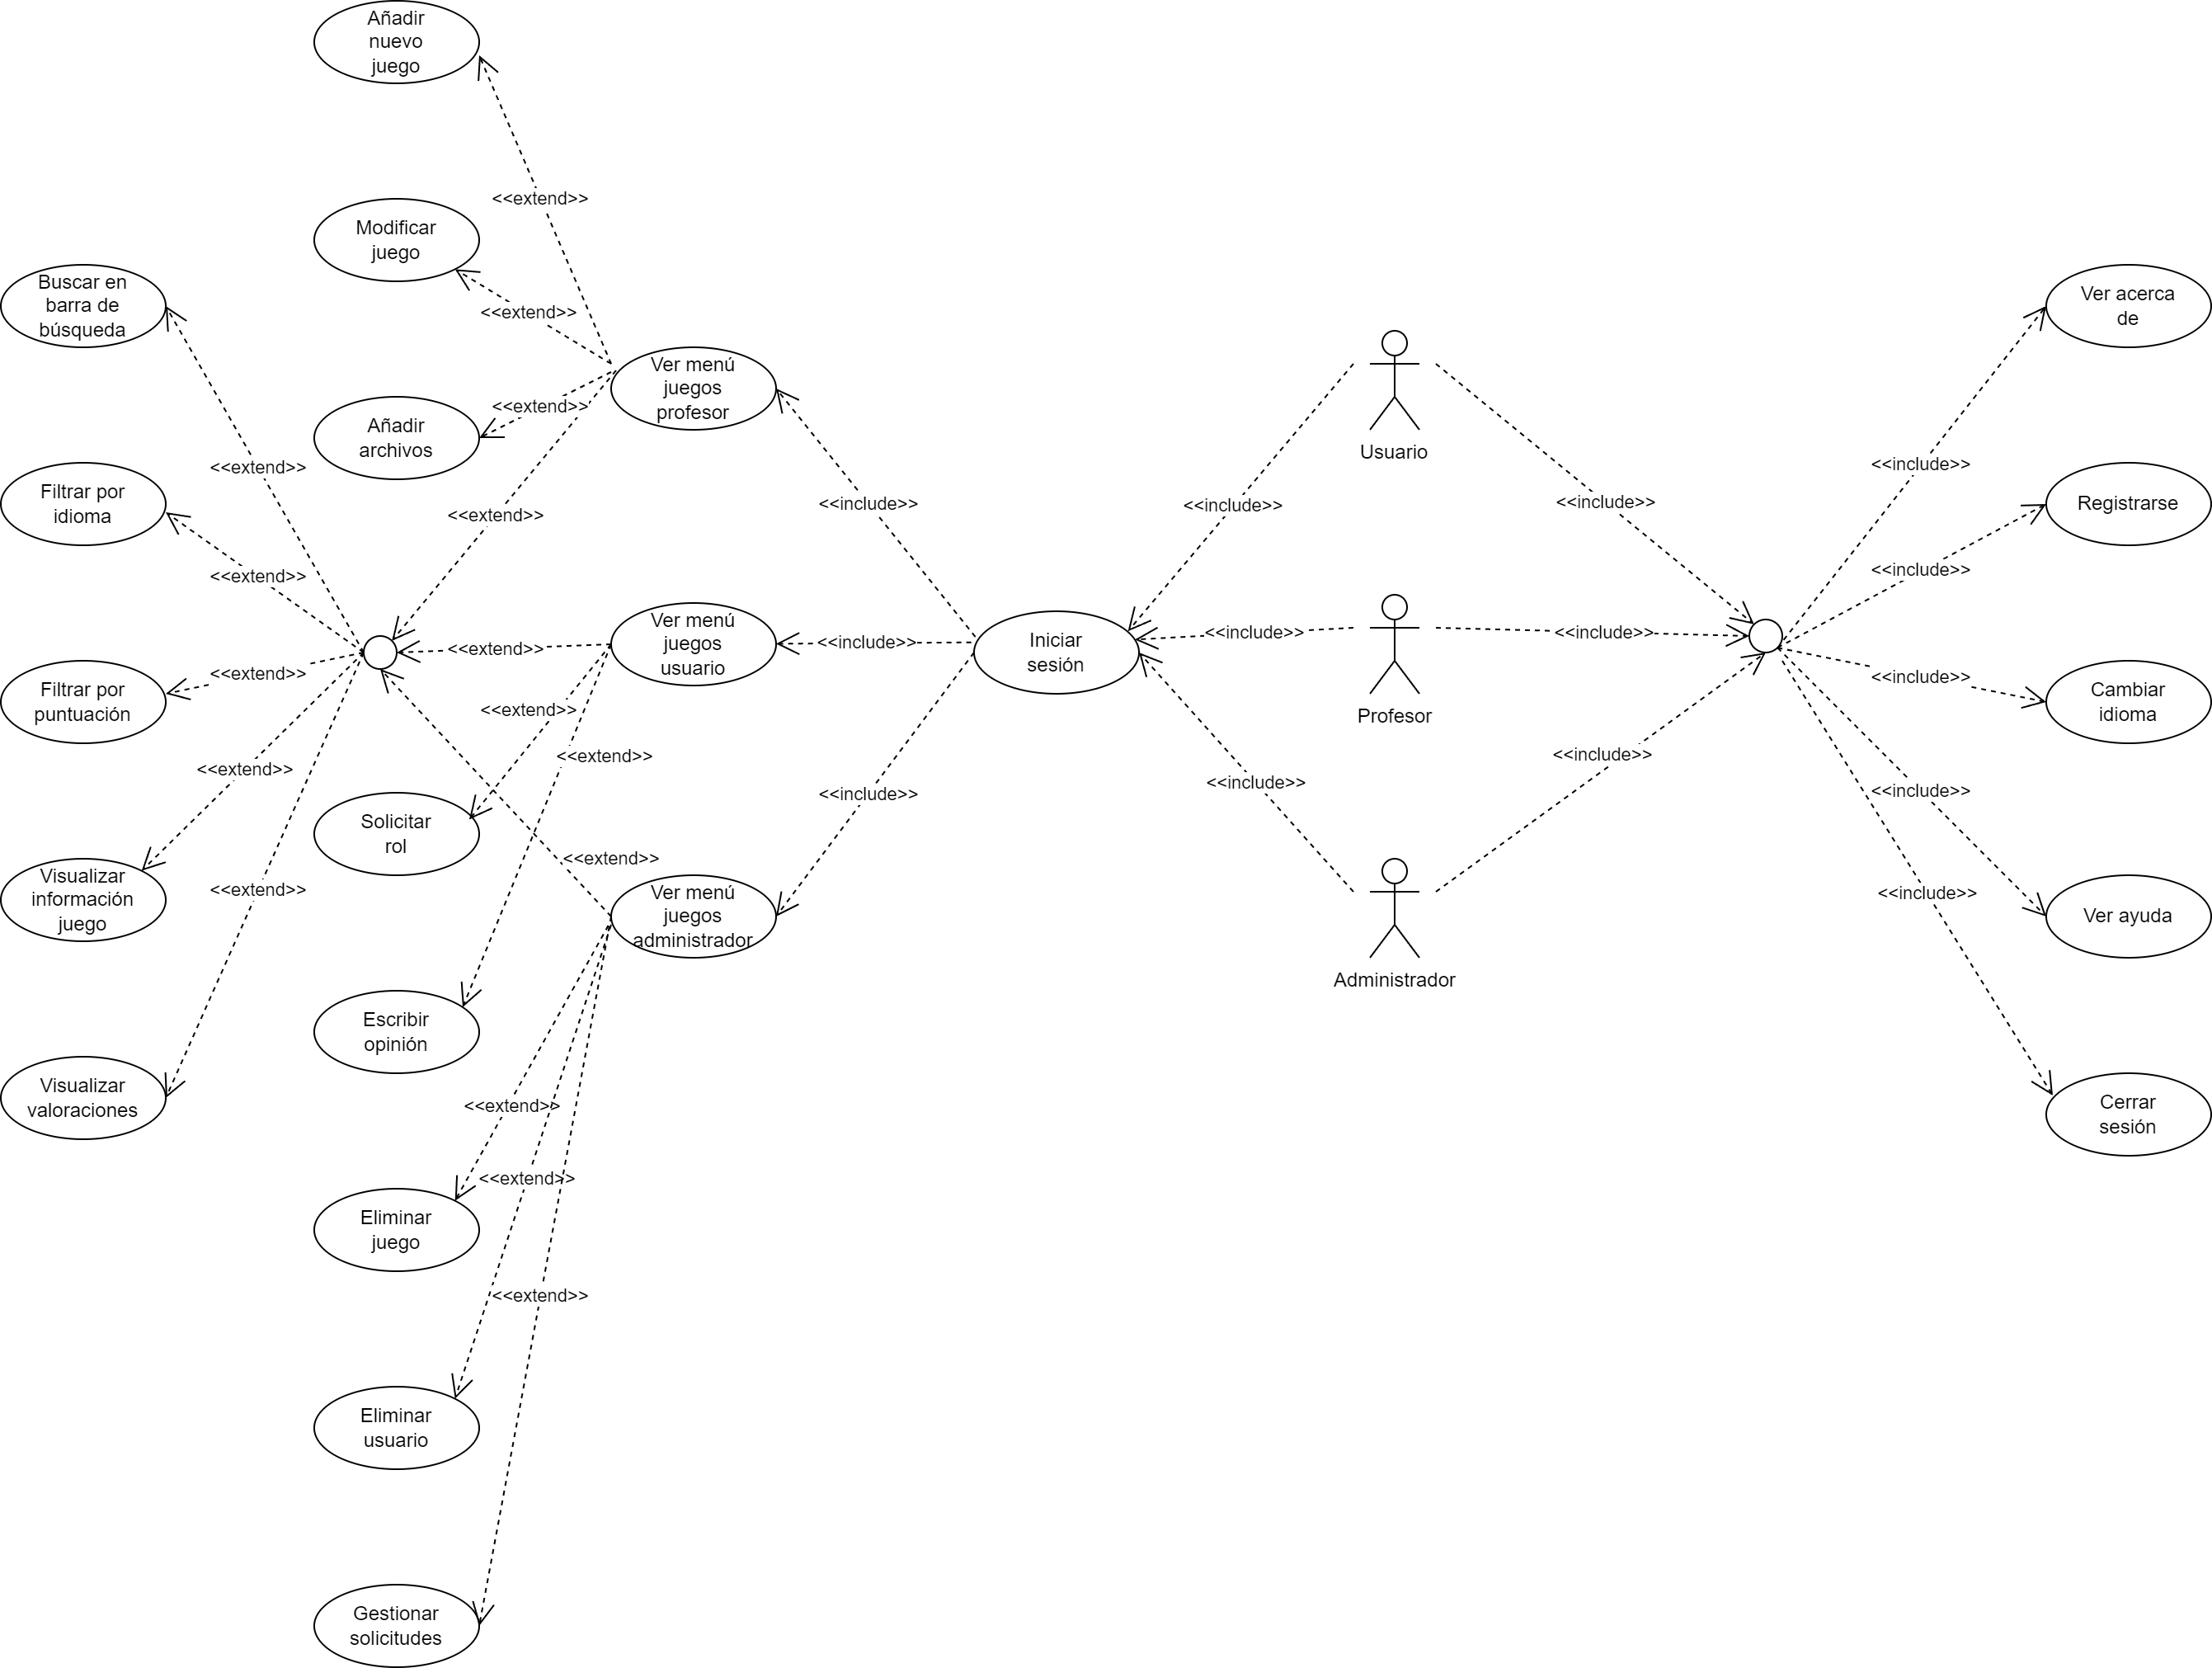
\includegraphics[scale=0.24]{img/diagramavf.png}
    \caption{Diagrama de casos de uso}
\end{figure}
\end{landscape}

\subsection{Tablas de casos de uso}
Las tablas de casos de uso del proyecto son las siguientes:
% Caso de Uso 1 -> Ver acerca de.
\begin{table}[h!]
	\centering
	\begin{tabularx}{\linewidth}{ p{0.21\columnwidth} p{0.71\columnwidth} }
		\toprule
		\textbf{CU-01}    & \textbf{Ver acerca de}\\
		\toprule
		\textbf{Versión}              & 1.0    \\
		\textbf{Autor}                & Usuario, profesor y administrador. \\
		\textbf{Requisitos asociados} & RF-1\\
		\textbf{Descripción}          & Permite al usuario obtener información general acerca de la aplicación. \\
		\textbf{Precondiciones}         & - \\
		\textbf{Acciones}             &
		\begin{enumerate}
			\def\labelenumi{\arabic{enumi}.}
			\tightlist
			\item El usuario pulsa el botón de ``Acerca de`` en la cabecera.
		\end{enumerate}\\
         \textbf{Postcondición}             & - \\
		\textbf{Excepciones}             & - \\
		\textbf{Importancia}          & Baja. \\
		\bottomrule
	\end{tabularx}
	\caption{CU-01 Ver acerca de.}
\end{table}

% Caso de Uso 2 ->Registrarse.
\begin{table}[h!]
	\centering
	\begin{tabularx}{\linewidth}{ p{0.21\columnwidth} p{0.71\columnwidth} }
		\toprule
		\textbf{CU-02}    & \textbf{Registrarse}\\
		\toprule
		\textbf{Versión}              & 1.0    \\
		\textbf{Autor}                & Usuario \\
		\textbf{Requisitos asociados} & RF-2\\
		\textbf{Descripción}          & Permite al usuario registrar su nueva cuenta. \\
		\textbf{Precondiciones}         & La base de datos debe estar disponible. \\
		\textbf{Acciones}             &
		\begin{enumerate}
			\def\labelenumi{\arabic{enumi}.}
			\tightlist
			\item El usuario accede a la opción de registrarse.
			\item El usuario introduce su nombre de usuario, nombre, apellido, institución y contraseña.
            \item El usuario pulsa el botón de crear cuenta.
		\end{enumerate}\\
         \textbf{Postcondiciones}             &
		\begin{enumerate}
			\def\labelenumi{\arabic{enumi}.}
			\tightlist
			\item El nombre del usuario no debe existir en la base de datos.
			\item La contraseña debe contener al menos 8 caracteres, una mayúscula, una minúscula y un símbolo.
            \item Todos los campos deben ser rellenados excepto el de la institución que es opcional.
		\end{enumerate}\\
		\textbf{Excepciones}             &
		\begin{enumerate}
			\def\labelenumi{\arabic{enumi}.}
			\tightlist
			\item El nombre de usuario ya existe (mensaje).
			\item El campo es requerido (mensaje).
            \item La contraseña debe contener al menos 8 caracteres, una mayúscula, una minúscula y un símbolo (mensaje).
            \item Las contraseñas ingresadas no coinciden (mensaje).
		\end{enumerate}\\
		\textbf{Importancia}          & Alta. \\
		\bottomrule
	\end{tabularx}
	\caption{CU-02 Registrarse.}
\end{table}


% Caso de Uso 3 -> Iniciar sesión.
\begin{table}[h!]
	\centering
	\begin{tabularx}{\linewidth}{ p{0.21\columnwidth} p{0.71\columnwidth} }
		\toprule
		\textbf{CU-03}    & \textbf{Iniciar sesión}\\
		\toprule
		\textbf{Versión}              & 1.0    \\
		\textbf{Autor}                & Usuario, profesor y administrador. \\
		\textbf{Requisitos asociados} & RF-3\\
		\textbf{Descripción}          & Permite al usuario iniciar sesión de su cuenta. \\
		\textbf{Precondiciones}         & El usuario debe estar registrado. \\
		\textbf{Acciones}             &
		\begin{enumerate}
			\def\labelenumi{\arabic{enumi}.}
			\tightlist
			\item El usuario accede a la opción de iniciar sesión o comenzar.
			\item El usuario introduce su nombre de usuario y contraseña.
            \item El usuario pulsa el botón de Iniciar sesión.
            \item El sistema verifica y autentica las credenciales del usuario.
		\end{enumerate}\\
         \textbf{Postcondiciones}             &
		\begin{enumerate}
			\def\labelenumi{\arabic{enumi}.}
			\tightlist
			\item El nombre del usuario y la contraseña deben existir en la base de datos.
		\end{enumerate}\\
		\textbf{Excepciones}             &
		\begin{enumerate}
			\def\labelenumi{\arabic{enumi}.}
			\tightlist
			\item El nombre de usuario o contraseña no son correctos (mensaje).
			\item Ha introducido la contraseña incorrecta más de tres veces. Cuenta bloqueada. (mensaje).
		\end{enumerate}\\
		\textbf{Importancia}          & Alta. \\
		\bottomrule
	\end{tabularx}
	\caption{CU-03 Iniciar sesión.}
\end{table}

% Caso de Uso 4 -> Ver menú juegos usuario.
\begin{table}[h!]
	\centering
	\begin{tabularx}{\linewidth}{ p{0.21\columnwidth} p{0.71\columnwidth} }
		\toprule
		\textbf{CU-04}    & \textbf{Ver menú juegos usuario}\\
		\toprule
		\textbf{Versión}              & 1.0    \\
		\textbf{Autor}                & Usuario. \\
		\textbf{Requisitos asociados} & RF-4, RF-4.1, RF.4.2, RF.4.3, RF.4.4, RF.4.5, RF.4.6, RF.4.7 \\
		\textbf{Descripción}          & Permite al usuario navegar por el menú de juegos, permitiéndole hacer búsquedas, aplicar filtros y ver más información y las valoraciones de los juegos, añadir una opinión y solicitar el rol de profesor.\\
		\textbf{Precondiciones}         & El usuario debe haber iniciado sesión como usuario. \\
		\textbf{Acciones}             &
		\begin{enumerate}
			\def\labelenumi{\arabic{enumi}.}
			\tightlist
			\item El usuario inicia sesión.
            \item El sistema verifica y autentica las credenciales del usuario.
            \item El usuario es redireccionado al menú de juegos.
            \item El sistema muestra las tarjetas de información de los juegos disponibles.
            \item El usuario puede realizar una búsqueda mediante barra de búsqueda o por filtros.
            \item El sistema puede mostrar los resultados de acuerdo con la búsqueda.
            \item El profesor puede pulsar el botón de ver más información del juego.
            \item El profesor puede pulsar el botón de ver las valoraciones del juego.
            \item El usuario puede añadir una opinión a cada juego.
            \item El usuario puede pulsar el botón de contacto para solicitar el rol de profesor.
		\end{enumerate}\\
         \textbf{Postcondición}             & El resultado de la búsqueda debe existir en la base de datos. \\
		\textbf{Excepciones}             &
		\begin{enumerate}
			\def\labelenumi{\arabic{enumi}.}
			\tightlist
			\item No se han encontrado resultados de búsqueda. (mensaje).
		\end{enumerate}\\
		\textbf{Importancia}          & Alta. \\
		\bottomrule
	\end{tabularx}
	\caption{CU-04 Ver menú juegos usuario.}
\end{table}

% Caso de Uso 5 -> Escribir opinión.
\begin{table}[h!]
	\centering
	\begin{tabularx}{\linewidth}{ p{0.21\columnwidth} p{0.71\columnwidth} }
		\toprule
		\textbf{CU-05}    & \textbf{Escribir opinión}\\
		\toprule
		\textbf{Versión}              & 1.0    \\
		\textbf{Autor}                & Usuario. \\
		\textbf{Requisitos asociados} & RF-4, RF.4.3 \\
		\textbf{Descripción}          & Permite al usuario escribir una opinión sobre cada juegos, puntuándolo y dejando una reseña.\\
		\textbf{Precondiciones}         & El usuario debe haber iniciado sesión como usuario. \\
		\textbf{Acciones}             &
		\begin{enumerate}
			\def\labelenumi{\arabic{enumi}.}
			\tightlist
		\item El usuario inicia sesión.
            \item El sistema verifica y autentica las credenciales del usuario.
            \item El usuario es redireccionado al menú de juegos.
            \item El usuario pulsa al botón de escribir opinión.
            \item El usuario selecciona la puntuación.
            \item El usuario escribe una reseña.
            \item El usuario pulsa el botón de enviar opinión.
            \item El usuario es redireccionado al menú de juegos.
		\end{enumerate}\\
         \textbf{Postcondición}             & - \\
		\textbf{Excepciones}             & - \\
		\textbf{Importancia}          & Media. \\
		\bottomrule
	\end{tabularx}
	\caption{CU-05 Escribir opinión.}
\end{table}

% Caso de Uso 6 -> Solicitar rol.
\begin{table}[h!]
	\centering
	\begin{tabularx}{\linewidth}{ p{0.21\columnwidth} p{0.71\columnwidth} }
		\toprule
		\textbf{CU-06}    & \textbf{Solicitar rol}\\
		\toprule
		\textbf{Versión}              & 1.0    \\
		\textbf{Autor}                & Usuario. \\
		\textbf{Requisitos asociados} & RF-4, RF.4.4 \\
		\textbf{Descripción}          & Permite al usuario solicitar el rol de profesor.\\
		\textbf{Precondiciones}         & El usuario debe haber iniciado sesión como usuario. \\
		\textbf{Acciones}             &
		\begin{enumerate}
			\def\labelenumi{\arabic{enumi}.}
			\tightlist
			\item El usuario inicia sesión.
            \item El sistema verifica y autentica las credenciales del usuario.
            \item El usuario es redireccionado al menú de juegos.
            \item El usuario pulsa al botón de contacto.
            \item El sistema muestra un mensaje con la explicación de cómo solicitar el rol.
            \item El usuario pulsa el botón de solicitar rol.
            \item El sistema muestra un mensaje de éxito
		\end{enumerate}\\
         \textbf{Postcondición}             & - \\
		\textbf{Excepciones}             & - \\
		\textbf{Importancia}          & Media. \\
		\bottomrule
	\end{tabularx}
	\caption{CU-06 Solicitar rol.}
\end{table}

% Caso de Uso 7 -> Ver menú juegos administrador.
\begin{table}[h!]
	\centering
	\begin{tabularx}{\linewidth}{ p{0.21\columnwidth} p{0.71\columnwidth} }
		\toprule
		\textbf{CU-07}    & \textbf{Ver menú juegos administrador}\\
		\toprule
		\textbf{Versión}              & 1.0    \\
		\textbf{Autor}                & Administrador. \\
		\textbf{Requisitos asociados} & RF-5, RF-5.1, RF.5.2, RF.5.3, RF.5.4, RF.5.5, RF.5.6, RF.5.7, RF.5.8 \\
		\textbf{Descripción}          & Permite al administrador navegar por el menú de juegos, permitiéndole hacer búsquedas, aplicar filtros y ver más información y las valoraciones de los juegos, eliminar un usuario, eliminar un juego y gestionar las solicitudes.\\
		\textbf{Precondiciones}         & El usuario debe haber iniciado sesión como administrador. \\
		\textbf{Acciones}             &
		\begin{enumerate}
			\def\labelenumi{\arabic{enumi}.}
			\tightlist
			\item El administrador inicia sesión.
            \item El sistema verifica y autentica las credenciales del administrador.
            \item El administrador es redireccionado al menú de juegos.
            \item El sistema muestra las tarjetas de información de los juegos disponibles.
            \item El administrador puede realizar una búsqueda mediante barra de búsqueda o por filtros.
            \item El sistema puede mostrar los resultados de acuerdo con la búsqueda.
            \item El profesor puede pulsar el botón de ver más información del juego.
            \item El profesor puede pulsar el botón de ver las valoraciones del juego.
            \item El administrador puede eliminar un juego.
            \item El administrador puede eliminar un usuario.
            \item El administrador puede gestionar las solicitudes.
		\end{enumerate}\\
         \textbf{Postcondición}             & El resultado de la búsqueda debe existir en la base de datos. \\
		\textbf{Excepciones}             &
		\begin{enumerate}
			\def\labelenumi{\arabic{enumi}.}
			\tightlist
			\item No se han encontrado resultados de búsqueda. (mensaje).
		\end{enumerate}\\
		\textbf{Importancia}          & Alta. \\
		\bottomrule
	\end{tabularx}
	\caption{CU-07 Ver menú juegos administrador.}
\end{table}

% Caso de Uso 8 -> Eliminar juego.
\begin{table}[h!]
	\centering
	\begin{tabularx}{\linewidth}{ p{0.21\columnwidth} p{0.71\columnwidth} }
		\toprule
		\textbf{CU-08}    & \textbf{Eliminar juego}\\
		\toprule
		\textbf{Versión}              & 1.0    \\
		\textbf{Autor}                & Administrador. \\
		\textbf{Requisitos asociados} & RF-5, RF.5.3 \\
		\textbf{Descripción}          & Permite al usuario eliminar un juego docente del sistema.\\
		\textbf{Precondiciones}         & El usuario debe haber iniciado sesión como administrador. \\
		\textbf{Acciones}             &
		\begin{enumerate}
			\def\labelenumi{\arabic{enumi}.}
			\tightlist
			\item El administrador inicia sesión.
            \item El sistema verifica y autentica las credenciales del administrador.
            \item El administrador es redireccionado al menú de juegos.
            \item El administrador pulsa al botón de administración.
            \item El administrador pulsa al botón de gestión de juegos.
            \item El sistema muestra una lista de juegos docentes existentes.
    	\item El administrador selecciona un juego docente para eliminar.
    	\item El sistema marca el juego docente como borrado en la base de datos.
		\end{enumerate}\\
         \textbf{Postcondición}             & - \\
		\textbf{Excepciones}             & - \\
		\textbf{Importancia}          & Media. \\
		\bottomrule
	\end{tabularx}
	\caption{CU-08 Eliminar juego.}
\end{table}

% Caso de Uso 9 -> Eliminar usuario.
\begin{table}[h!]
	\centering
	\begin{tabularx}{\linewidth}{ p{0.21\columnwidth} p{0.71\columnwidth} }
		\toprule
		\textbf{CU-09}    & \textbf{Eliminar usuario}\\
		\toprule
		\textbf{Versión}              & 1.0    \\
		\textbf{Autor}                & Administrador. \\
		\textbf{Requisitos asociados} & RF-5, RF.5.4 \\
		\textbf{Descripción}          & Permite al usuario eliminar un usuario del sistema.\\
		\textbf{Precondiciones}         & El usuario debe haber iniciado sesión como administrador. \\
		\textbf{Acciones}             &
		\begin{enumerate}
			\def\labelenumi{\arabic{enumi}.}
			\tightlist
			\item El administrador inicia sesión.
            \item El sistema verifica y autentica las credenciales del administrador.
            \item El administrador es redireccionado al menú de juegos.
            \item El administrador pulsa al botón de administración.
            \item El administrador pulsa al botón de gestión de usuarios.
            \item El sistema muestra una lista de los usuarios existentes.
    	\item El administrador selecciona un usuario para eliminar.
    	\item El sistema marca el usuario como borrado en la base de datos.
		\end{enumerate}\\
         \textbf{Postcondición}             & - \\
		\textbf{Excepciones}             & - \\
		\textbf{Importancia}          & Media. \\
		\bottomrule
	\end{tabularx}
	\caption{CU-09 Eliminar usuario.}
\end{table}

% Caso de Uso 10 -> Gestionar solicitudes.
\begin{table}[h!]
	\centering
	\begin{tabularx}{\linewidth}{ p{0.21\columnwidth} p{0.71\columnwidth} }
		\toprule
		\textbf{CU-10}    & \textbf{Gestionar solicitudes}\\
		\toprule
		\textbf{Versión}              & 1.0    \\
		\textbf{Autor}                & Administrador. \\
		\textbf{Requisitos asociados} & RF-5, RF.5.5 \\
		\textbf{Descripción}          & Permite al usuario gestionar las solicitudes pendientes del sismtea.\\
		\textbf{Precondiciones}         & El usuario debe haber iniciado sesión como administrador. \\
		\textbf{Acciones}             &
		\begin{enumerate}
			\def\labelenumi{\arabic{enumi}.}
			\tightlist
			\item El administrador inicia sesión.
            \item El sistema verifica y autentica las credenciales del administrador.
            \item El administrador es redireccionado al menú de juegos.
            \item El administrador pulsa al botón de administración.
            \item El administrador pulsa al botón de gestión de solicitudes.
            \item El sistema muestra una lista de las solicitudes pendientes.
    	\item El administrador acepta o rechaza una solicitud.
    	\item El sistema marca la solicitud como aceptada o rechazada en la base de datos.
		\end{enumerate}\\
         \textbf{Postcondición}             & - \\
		\textbf{Excepciones}             & - \\
		\textbf{Importancia}          & Media. \\
		\bottomrule
	\end{tabularx}
	\caption{CU-10 Gestionar solicitudes.}
\end{table}

% Caso de Uso 11 -> Ver menú juegos profesor.
\begin{table}[h!]
	\centering
	\begin{tabularx}{\linewidth}{ p{0.21\columnwidth} p{0.71\columnwidth} }
		\toprule
		\textbf{CU-11}    & \textbf{Ver menú juegos profesor}\\
		\toprule
		\textbf{Versión}              & 1.0    \\
		\textbf{Autor}                & Profesor. \\
		\textbf{Requisitos asociados} & RF-6, RF-6.1, RF.6.2, RF.6.3, RF.6.4, RF.6.5, RF.6.6, RF.6.7, RF.6.8 \\
		\textbf{Descripción}          & Permite al profesor navegar por el menú de juegos, permitiéndole hacer búsquedas, aplicar filtros y ver más información y las valoraciones de los juegos, añadir un nuevo juego, modificar un juego existente y añadir archivos a los juegos.\\
		\textbf{Precondiciones}         & El usuario debe haber iniciado sesión como profesor. \\
		\textbf{Acciones}             &
		\begin{enumerate}
			\def\labelenumi{\arabic{enumi}.}
			\tightlist
			\item El profesor inicia sesión.
            \item El sistema verifica y autentica las credenciales del profesor.
            \item El profesor es redireccionado al menú de juegos.
            \item El sistema muestra las tarjetas de información de los juegos disponibles.
            \item El profesor puede realizar una búsqueda mediante barra de búsqueda o por filtros.
            \item El sistema puede mostrar los resultados de acuerdo con la búsqueda.
            \item El profesor puede pulsar el botón de ver más información del juego.
            \item El profesor puede pulsar el botón de ver las valoraciones del juego.
            \item El profesor puede añadir un nuevo juego.
            \item El profesor puede modificar un juego.
            \item El profesor puede añadir archivos a los juegos.
		\end{enumerate}\\
         \textbf{Postcondición}             & El resultado de la búsqueda debe existir en la base de datos. \\
		\textbf{Excepciones}             &
		\begin{enumerate}
			\def\labelenumi{\arabic{enumi}.}
			\tightlist
			\item No se han encontrado resultados de búsqueda. (mensaje).
		\end{enumerate}\\
		\textbf{Importancia}          & Alta. \\
		\bottomrule
	\end{tabularx}
	\caption{CU-11 Ver menú juegos profesor.}
\end{table}

% Caso de Uso 12 -> Añadir nuevo juego.
\begin{table}[h!]
	\centering
	\begin{tabularx}{\linewidth}{ p{0.21\columnwidth} p{0.71\columnwidth} }
		\toprule
		\textbf{CU-12}    & \textbf{Añadir nuevo juego}\\
		\toprule
		\textbf{Versión}              & 1.0    \\
		\textbf{Autor}                & Profesor. \\
		\textbf{Requisitos asociados} & RF-6, RF.6.3 \\
		\textbf{Descripción}          & Permite al profesor añadir un nuevo juego.\\
		\textbf{Precondiciones}         & El usuario debe haber iniciado sesión como profesor. \\
		\textbf{Acciones}             &
		\begin{enumerate}
			\def\labelenumi{\arabic{enumi}.}
			\tightlist
			\item El profesor inicia sesión.
            \item El sistema verifica y autentica las credenciales del profesor.
            \item El profesor es redireccionado al menú de juegos.
            \item El profesor pulsa el botón de añadir juego.
            \item El sistema muestra un formulario para ingresar los datos del nuevo juego.
    	\item El profesor completa los campos del formulario.
    	\item El sistema almacena los datos del nuevo juego en la base de datos.
		\end{enumerate}\\
         \textbf{Postcondición}             & Todos los campos requeridos deben ser rellenados. \\
		\textbf{Excepciones}             & - \\
		\textbf{Importancia}          & Alta. \\
		\bottomrule
	\end{tabularx}
	\caption{CU-12 Añadir nuevo juego.}
\end{table}

% Caso de Uso 13 -> Modificar juego.
\begin{table}[h!]
	\centering
	\begin{tabularx}{\linewidth}{ p{0.21\columnwidth} p{0.71\columnwidth} }
		\toprule
		\textbf{CU-13}    & \textbf{Modificar juego}\\
		\toprule
		\textbf{Versión}              & 1.0    \\
		\textbf{Autor}                & Profesor. \\
		\textbf{Requisitos asociados} & RF-6, RF.6.4 \\
		\textbf{Descripción}          & Permite al profesor modificar un juego ya existente.\\
		\textbf{Precondiciones}         & El usuario debe haber iniciado sesión como profesor. \\
		\textbf{Acciones}             &
		\begin{enumerate}
			\def\labelenumi{\arabic{enumi}.}
			\tightlist
			\item El profesor inicia sesión.
            \item El sistema verifica y autentica las credenciales del profesor.
            \item El profesor es redireccionado al menú de juegos.
    	\item El profesor selecciona un juego docente para modificar.
            \item El profesor pulsa el botón de modificar juego.
    	\item El sistema muestra el formulario con los datos actuales del juego.
    	\item El profesor realiza las modificaciones necesarias en el formulario.
            \item El sistema actualiza los datos del juego docente en la base de datos.
		\end{enumerate}\\
         \textbf{Postcondición}             & Todos los campos requeridos deben ser rellenados. \\
		\textbf{Excepciones}             & - \\
		\textbf{Importancia}          & Alta. \\
		\bottomrule
	\end{tabularx}
	\caption{CU-13 Modificar juego.}
\end{table}

% Caso de Uso 14 -> Añadir archivos.
\begin{table}[h!]
	\centering
	\begin{tabularx}{\linewidth}{ p{0.21\columnwidth} p{0.71\columnwidth} }
		\toprule
		\textbf{CU-14}    & \textbf{Añadir archivos}\\
		\toprule
		\textbf{Versión}              & 1.0    \\
		\textbf{Autor}                & Profesor. \\
		\textbf{Requisitos asociados} & RF-6, RF.6.5 \\
		\textbf{Descripción}          & Permite al profesor añadir archivos a los juegos.\\
		\textbf{Precondiciones}         & El usuario debe haber iniciado sesión como profesor. \\
		\textbf{Acciones}             &
		\begin{enumerate}
			\def\labelenumi{\arabic{enumi}.}
			\tightlist
			\item El profesor inicia sesión.
            \item El sistema verifica y autentica las credenciales del profesor.
            \item El profesor es redireccionado al menú de juegos.
    	\item El profesor selecciona un juego docente al que añadir archivos.
            \item El sistema muestra una interfaz de carga de archivos.
    	\item El profesor selecciona uno o varios archivos y los sube al sistema.
    	\item El sistema almacena los archivos en el sistema.
		\end{enumerate}\\
         \textbf{Postcondición}             & - \\
		\textbf{Excepciones}             & - \\
		\textbf{Importancia}          & Media. \\
		\bottomrule
	\end{tabularx}
	\caption{CU-14 Añadir archivos.}
\end{table}

% Caso de Uso 15 -> Buscar en barra de búsqueda.
\begin{table}[h!]
	\centering
	\begin{tabularx}{\linewidth}{ p{0.21\columnwidth} p{0.71\columnwidth} }
		\toprule
		\textbf{CU-15}    & \textbf{Buscar en barra de búsqueda}\\
		\toprule
		\textbf{Versión}              & 1.0    \\
		\textbf{Autor}                & Usuario, profesor y administrador. \\
		\textbf{Requisitos asociados} & RF-4, RF-4.5, RF-5, RF-5.6, RF-6, RF-6.6 \\
		\textbf{Descripción}          & Permite al usuario, profesor o administrado buscar juegos mediante la barra de búsqueda.\\
		\textbf{Precondiciones}         & El usuario debe haber iniciado sesión. \\
		\textbf{Acciones}             &
		\begin{enumerate}
			\def\labelenumi{\arabic{enumi}.}
			\tightlist
			\item El usuario inicia sesión.
            \item El sistema verifica y autentica las credenciales del usuario.
            \item El usuario es redireccionado al menú de juegos.
            \item El sistema muestra una barra de búsqueda y opciones de filtro por idioma y puntuación.
            \item El usuario puede introducir texto en la barra de búsqueda para realizar una búsqueda personalizada.
            \item El sistema muestra los resultados correspondientes a la búsqueda realizada.
		\end{enumerate}\\
         \textbf{Postcondición}             & El resultado de la búsqueda debe existir en la base de datos. \\
		\textbf{Excepciones}             &
		\begin{enumerate}
			\def\labelenumi{\arabic{enumi}.}
			\tightlist
			\item No se han encontrado resultados de búsqueda. (mensaje).
		\end{enumerate}\\
		\textbf{Importancia}          & Media. \\
		\bottomrule
	\end{tabularx}
	\caption{CU-15 Buscar en barra de búsqueda.}
\end{table}

% Caso de Uso 16 -> Filtrar por idioma.
\begin{table}[h!]
	\centering
	\begin{tabularx}{\linewidth}{ p{0.21\columnwidth} p{0.71\columnwidth} }
		\toprule
		\textbf{CU-16}    & \textbf{Filtrar por idioma}\\
		\toprule
		\textbf{Versión}              & 1.0    \\
		\textbf{Autor}                & Usuario, profesor y administrador. \\
		\textbf{Requisitos asociados} & RF-4, RF-4.6, RF-5, RF-5.7, RF-6, RF-6.7 \\
		\textbf{Descripción}          & Permite al usuario, profesor o administrado buscar juegos mediante la aplicación de filtros por idioma.\\
		\textbf{Precondiciones}         & El usuario debe haber iniciado sesión. \\
		\textbf{Acciones}             &
		\begin{enumerate}
			\def\labelenumi{\arabic{enumi}.}
			\tightlist
			\item El usuario inicia sesión.
            \item El sistema verifica y autentica las credenciales del usuario.
            \item El usuario es redireccionado al menú de juegos.
            \item El sistema muestra una barra de búsqueda y opciones de filtro por idioma y puntuación.
            \item El usuario de aplicar filtros por idioma para refinar la búsqueda.
            \item El sistema filtra los juegos según los criterios seleccionados y muestra los resultados actualizados.
		\end{enumerate}\\
         \textbf{Postcondición}             & El resultado de la búsqueda debe existir en la base de datos. \\
		\textbf{Excepciones}             &
		\begin{enumerate}
			\def\labelenumi{\arabic{enumi}.}
			\tightlist
			\item No se han encontrado resultados de búsqueda. (mensaje).
		\end{enumerate}\\
		\textbf{Importancia}          & Media. \\
		\bottomrule
	\end{tabularx}
	\caption{CU-16 Filtrar por idioma.}
\end{table}

% Caso de Uso 17 -> Filtrar por puntuación.
\begin{table}[h!]
	\centering
	\begin{tabularx}{\linewidth}{ p{0.21\columnwidth} p{0.71\columnwidth} }
		\toprule
		\textbf{CU-17}    & \textbf{Filtrar por puntuación}\\
		\toprule
		\textbf{Versión}              & 1.0    \\
		\textbf{Autor}                & Usuario, profesor y administrador. \\
		\textbf{Requisitos asociados} & RF-4, RF-4.7, RF-5, RF-5.8, RF-6, RF-6.8 \\
		\textbf{Descripción}          & Permite al usuario, profesor o administrado buscar juegos mediante la aplicación de filtros por puntuación.\\
		\textbf{Precondiciones}         & El usuario debe haber iniciado sesión. \\
		\textbf{Acciones}             &
		\begin{enumerate}
			\def\labelenumi{\arabic{enumi}.}
			\tightlist
			\item El usuario inicia sesión.
            \item El sistema verifica y autentica las credenciales del usuario.
            \item El usuario es redireccionado al menú de juegos.
            \item El sistema muestra una barra de búsqueda y opciones de filtro por idioma y puntuación.
            \item El usuario de aplicar filtros por puntuación para refinar la búsqueda.
            \item El sistema filtra los juegos según los criterios seleccionados y muestra los resultados actualizados.
		\end{enumerate}\\
         \textbf{Postcondición}             & El resultado de la búsqueda debe existir en la base de datos. \\
		\textbf{Excepciones}             &
		\begin{enumerate}
			\def\labelenumi{\arabic{enumi}.}
			\tightlist
			\item No se han encontrado resultados de búsqueda. (mensaje).
		\end{enumerate}\\
		\textbf{Importancia}          & Media. \\
		\bottomrule
	\end{tabularx}
	\caption{CU-17 Filtrar por puntuación.}
\end{table}

% Caso de Uso 18 -> Visualizar información juego.
\begin{table}[h!]
	\centering
	\begin{tabularx}{\linewidth}{ p{0.21\columnwidth} p{0.71\columnwidth} }
		\toprule
		\textbf{CU-18}    & \textbf{Visualizar información juego}\\
		\toprule
		\textbf{Versión}              & 1.0    \\
		\textbf{Autor}                & Usuario, profesor y administrador. \\
		\textbf{Requisitos asociados} & RF-4, RF-4.1, RF-5, RF-5.1, RF-6, RF-6.1 \\
		\textbf{Descripción}          & Permite al usuario, profesor o administrado visualizar la información más detallada de los juegos.\\
		\textbf{Precondiciones}         & El usuario debe haber iniciado sesión. \\
		\textbf{Acciones}             &
		\begin{enumerate}
			\def\labelenumi{\arabic{enumi}.}
			\tightlist
			\item El usuario inicia sesión.
            \item El sistema verifica y autentica las credenciales del usuario.
            \item El usuario es redireccionado al menú de juegos.
            \item El usuario pulsa el botón de ver más información del juego deseado.
            \item El sistema muestra la información detallada del juego.
		\end{enumerate}\\
         \textbf{Postcondición}             & - \\
		\textbf{Excepciones}             & - \\
		\textbf{Importancia}          & Alta. \\
		\bottomrule
	\end{tabularx}
	\caption{CU-18 Visualizar información juego.}
\end{table}

% Caso de Uso 19 -> Visualizar valoraciones.
\begin{table}[h!]
	\centering
	\begin{tabularx}{\linewidth}{ p{0.21\columnwidth} p{0.71\columnwidth} }
		\toprule
		\textbf{CU-19}    & \textbf{Visualizar valoraciones}\\
		\toprule
		\textbf{Versión}              & 1.0    \\
		\textbf{Autor}                & Usuario, profesor y administrador. \\
		\textbf{Requisitos asociados} & RF-4, RF-4.2, RF-5, RF-5.2, RF-6, RF-6.2 \\
		\textbf{Descripción}          & Permite al usuario, profesor o administrado visualizar las valoraciones de los juegos.\\
		\textbf{Precondiciones}         & El usuario debe haber iniciado sesión. \\
		\textbf{Acciones}             &
		\begin{enumerate}
			\def\labelenumi{\arabic{enumi}.}
			\tightlist
			\item El usuario inicia sesión.
            \item El sistema verifica y autentica las credenciales del usuario.
            \item El usuario es redireccionado al menú de juegos.
            \item El usuario pulsa el botón de ver las valoraciones del juego deseado.
            \item El sistema muestra las valoraciones del juego.
		\end{enumerate}\\
         \textbf{Postcondición}             & - \\
		\textbf{Excepciones}             & - \\
		\textbf{Importancia}          & Media. \\
		\bottomrule
	\end{tabularx}
	\caption{CU-19 Visualizar valoraciones.}
\end{table}

% Caso de Uso 20 ->  Cambiar idioma.
\begin{table}[h!]
	\centering
	\begin{tabularx}{\linewidth}{ p{0.21\columnwidth} p{0.71\columnwidth} }
		\toprule
		\textbf{CU-20}    & \textbf{Cambiar idioma}\\
		\toprule
		\textbf{Versión}              & 1.0    \\
		\textbf{Autor}                & Usuario, profesor y administrador. \\
		\textbf{Requisitos asociados} & RF-7\\
		\textbf{Descripción}          & Permite al usuario cambiar el idioma de la aplicación. \\
		\textbf{Precondiciones}         & - \\
		\textbf{Acciones}             &
		\begin{enumerate}
			\def\labelenumi{\arabic{enumi}.}
			\tightlist
			\item El sistema muestra las opciones de idioma.
			\item El usuario selecciona el idioma deseado.
            \item El sistema actualiza el idioma de la aplicación según la selección del usuario.
		\end{enumerate}\\
         \textbf{Postcondiciones}             &
		\begin{enumerate}
			\def\labelenumi{\arabic{enumi}.}
			\tightlist
			\item Si el usuario no selecciona idioma, el idioma por defecto es el español.
		\end{enumerate}\\
		\textbf{Excepciones}             & - \\
		\textbf{Importancia}          & Baja. \\
		\bottomrule
	\end{tabularx}
	\caption{CU-20  Cambiar idioma.}
\end{table}

% Caso de Uso 21 ->  Ver ayuda.
\begin{table}[h!]
	\centering
	\begin{tabularx}{\linewidth}{ p{0.21\columnwidth} p{0.71\columnwidth} }
		\toprule
		\textbf{CU-21}    & \textbf{Ver ayuda}\\
		\toprule
		\textbf{Versión}              & 1.0    \\
		\textbf{Autor}                & Usuario, profesor y administrador. \\
		\textbf{Requisitos asociados} & RF-7\\
		\textbf{Descripción}          & Permite al usuario ver la ayuda mediante un manual. \\
		\textbf{Precondiciones}         & - \\
		\textbf{Acciones}             &
		\begin{enumerate}
			\def\labelenumi{\arabic{enumi}.}
			\tightlist
			\item El sistema muestra la opción de ayuda.
			\item El usuario pulsa el botón de ayuda.
            \item El sistema redirecciona al usuario al manual de ayuda.
		\end{enumerate}\\
         \textbf{Postcondiciones}             & - \\
		\textbf{Excepciones}             & - \\
		\textbf{Importancia}          & Baja. \\
		\bottomrule
	\end{tabularx}
	\caption{CU-21 Ver ayuda.}
\end{table}

% Caso de Uso 22 -> Cerrar sesión.
\begin{table}[h!]
	\centering
	\begin{tabularx}{\linewidth}{ p{0.21\columnwidth} p{0.71\columnwidth} }
		\toprule
		\textbf{CU-22}    & \textbf{Cerrar sesión}\\
		\toprule
		\textbf{Versión}              & 1.0    \\
		\textbf{Autor}                & Usuario, profesor y administrador. \\
		\textbf{Requisitos asociados} & RF-9 \\
		\textbf{Descripción}          & Permite al usuario cerrar la sesión de su cuenta. \\
		\textbf{Precondiciones}         & El usuario debe haber iniciado sesión. \\
		\textbf{Acciones}             &
		\begin{enumerate}
			\def\labelenumi{\arabic{enumi}.}
			\tightlist
			\item El usuario pulsa el botón de cerrar sesión en la cabecera.
            \item El sistema cierra la sesión del usuario y redirige a la pantalla de inicio.
		\end{enumerate}\\
         \textbf{Postcondición}             & - \\
		\textbf{Excepciones}             & - \\
		\textbf{Importancia}          & Alta. \\
		\bottomrule
	\end{tabularx}
	\caption{CU-22 Cerrar sesión.}
\end{table}

\apendice{Especificación de diseño}

\section{Introducción}
En este apartado se explica cómo se han estructurado los elementos que constituyen la aplicación, incluyendo sus datos, procedimientos, arquitectura e interfaces.

\section{Diseño de datos}
Para el diseño de datos del proyecto se ha empleado una estructura de base de datos bien definida, con el fin de organizar y almacenar la información de una forma eficiente. Por ello, la estructura de la base de datos es la siguiente:

\subsection{Estructura de la base de datos:}
Se ha utilizado PostgreSQL como sistema de gestión de bases de datos para la implementación del proyecto. 

La estructura de base de datos diseñada consta de cuatro tablas para almacenar la información:
\begin{itemize}
    \item \textbf{Usuarios:} la tabla usuarios contiene información sobre los usuarios registrados. Esta tabla almacena los siguientes campos para cada usuario:
        \begin{itemize}
        \tightlist
            \item \textbf{id:} identificador único de cada usuario, se trata de la clave primaria de la tabla y es un autoincremental.
            \item \textbf{usuario:} nombre que el usuario usa para iniciar sesión.
            \item \textbf{nombre:} nombre del usuario.
            \item \textbf{apellido:} apellido del usuario.
            \item \textbf{institución:} institución a la que pertenece el usuario. Este campo es opcional.
            \item \textbf{contraseña:} contraseña que el usuario utiliza para iniciar sesión. Se almacena hasheada. 
            \item \textbf{rol:} nivel de acceso que el usuario tiene en el sistema. Los posibles roles son \"administrador\", \"profesor\" y \"usuario\".
            \item \textbf{borrado:} indica si el usuario está borrado o no.
        \end{itemize}
    \item \textbf{Juegos:} la tabla juegos contiene toda la información sobre los juegos docentes registrados. Esta tabla almacena los siguientes campos para cada juego:
        \begin{itemize}
        \tightlist
            \item \textbf{id:} identificador único de cada juego, se trata de la clave primaria de la tabla y es un auto incremental.
            \item \textbf{nombre\_juego:} nombre del juego docente.
            \item \textbf{descripción:} descripción general del juego docente.
            \item \textbf{idioma:} idioma del juego docente.
            \item \textbf{enlace:} enlace de acceso al juego docente.
            \item \textbf{puntuación:} puntuación valorada por el profesor del juego.
            \item \textbf{disciplina:} disciplina del juego docente.
            \item \textbf{naturaleza:} naturaleza del juego docente, siendo online o descargable.
            \item \textbf{precio:} precio del juego docente, siendo gratuito o de pago.
            \item \textbf{instrucciones:} disponibilidad de las instrucciones del juego docente.
            \item \textbf{notas\_instructor:} disponibilidad de las notas instructor del juego docente.
            \item \textbf{objetivos:}  descripción sobre los objetivos generales del juego docente.
            \item \textbf{espacio\_control:} descripción sobre el espacio control del juego docente.
            \item \textbf{objetivos\_principales:}  descripción sobre los objetivos principales del juego docente.
            \item \textbf{objetivos\_secundarios:}  descripción sobre los objetivos secundarios del juego docente.
            \item \textbf{estructura\_sesiones:} descripción sobre la estructura sesiones del juego docente.
            \item \textbf{aspectos\_adicionales:} descripción sobre los aspectos adicionales del juego docente.
            \item \textbf{entretenimiento:} valoración numérica sobre el entretenimiento del juego docente.
            \item \textbf{aprendizaje:} valoración numérica sobre el aprendizaje del juego docente.
            \item \textbf{complejidad\_alumno:} valoración numérica sobre la complejidad del juego docente para los alumnos.
            \item \textbf{complejidad\_instructores:} valoración numérica sobre la complejidad del juego docente para los instructores.
            \item \textbf{youtube\_url:} url en la que se encuentra el vídeo tutorial de ayuda del juego docente.
            \item \textbf{id\_usuario\_creación:} id del usuario que realizó la  creación del juego docente.
            \item \textbf{fecha\_creación:} fecha y hora en la que se realizó la creación del juego docente.
            \item \textbf{id\_usuario\_modificación:} id del usuario que realizó la  modificación del juego docente.
            \item \textbf{fecha\_modificación:} fecha y hora en la que se realizó la  modificación del juego docente.

            \item \textbf{puntuacion\_media\_usuario:} puntuación media que tiene un juego a partir de las puntuaciones que le han dado los usuarios.
            \item \textbf{estrellas\_general:} número de estrellas que tiene un juego según la puntuación media que tiene el juego.
            \item \textbf{archivo\_instrucciones\_jugador:} nombre del archivo de las instrucciones del juego para el jugador.
            \item \textbf{archivo\_instrucciones\_instructor:} nombre del archivo de las instrucciones del juego para el instructor.
            \item \textbf{archivo\_juego:} nombre del archivo del juego.                                          \item \textbf{borrado:} indica si el juego está borrado o no.
        \end{itemize}

    \item \textbf{Solicitudes:} la tabla de las solicitudes contiene información sobre las solicitudes registradas. Esta tabla almacena los siguientes campos para cada solicitud:
        \begin{itemize}
        \tightlist
            \item \textbf{id:} identificador único de cada solicitud, se trata de la clave primaria de la tabla y es un auto incremental.
            \item \textbf{estado:} estado en el que se encuentra la solicitud de rol de profesor.
            \item \textbf{id\_usuario\_solicitud:} id del usuario que realizó la solicitud.
            \item \textbf{fecha\_solicitud:} fecha y hora en la que se realizó la solicitud.
        \end{itemize}

    \item \textbf{Valoraciones:} la tabla de las valoraciones contiene información sobre las valoraciones registradas. Esta tabla almacena los siguientes campos para cada valoración:
        \begin{itemize}
        \tightlist
            \item \textbf{id:} identificador único de cada valoración, se trata de la clave primaria de la tabla y es un auto incremental.
            \item \textbf{puntuacion:} puntuación que le da a un juego un usuario.
            \item \textbf{estrellas\_individual:} número de estrellas según la puntuación que un usuario da a un juego.
            \item \textbf{comentario:} comentario que el usuario realiza sobre el juego.
            \item \textbf{fecha\_valoracion:} fecha y hora en la que se realizó la valoración.
            \item \textbf{id\_usuario\_valoracion:} id del usuario que realizó la valoración.
            \item \textbf{id\_juego:} id del juego al que se realizó la valoración.
        \end{itemize}
\end{itemize}

A continuación, se muestra el modelo de entidad-relación (ERD) que representa de forma visual las entidades en la base de datos y las relaciones entre ellas.
\newpage

\begin{figure}[!h]
\centering
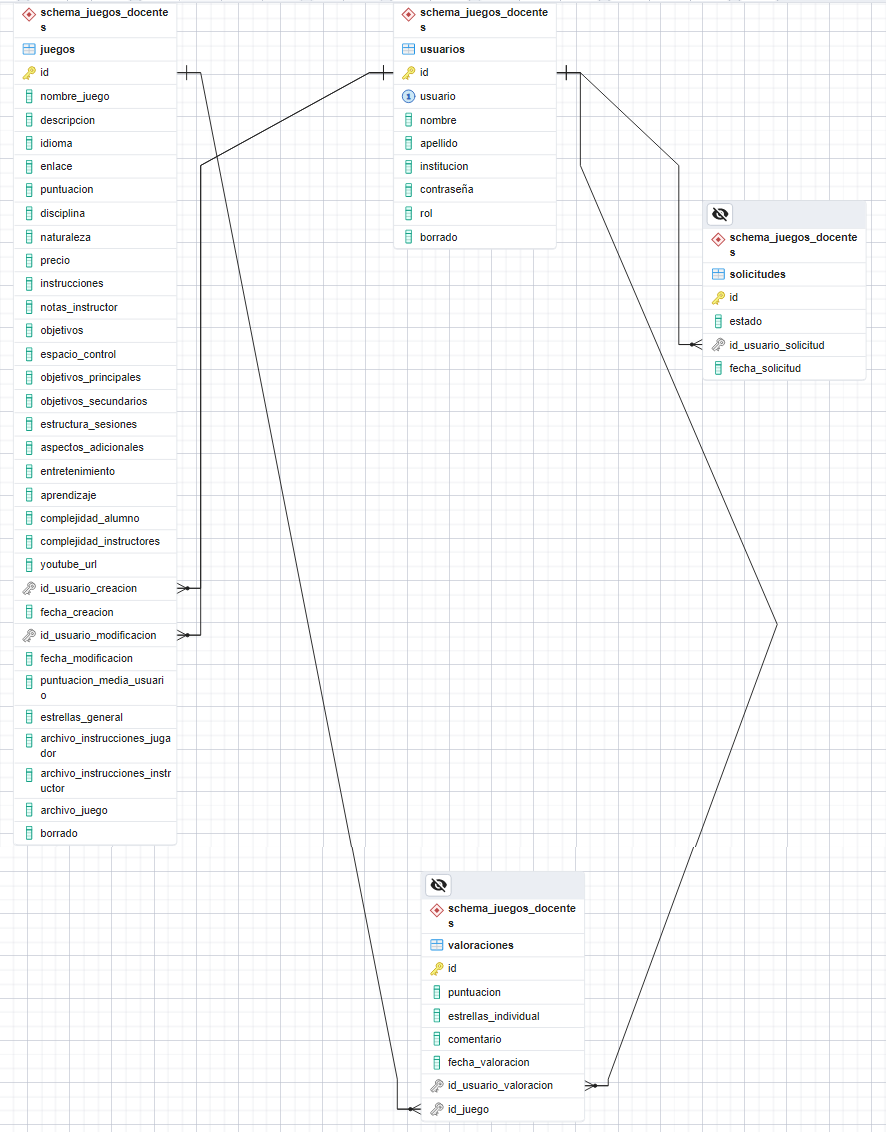
\includegraphics[width=1.0\textwidth]{ERD}
\caption{Modelo ERD.}
\label{fig:ERD}
\end{figure}

\newpage
\section{Diseño procedimental}
En esta sección se presentan los diagramas de secuencia de la aplicación, los cuales ilustran el funcionamiento y la interacción entre los diferentes componentes de la aplicación. 

\subsection{Registro}
Se muestra el diagrama de secuencia en la ejecución del registro.

\begin{figure}[!h]
\centering
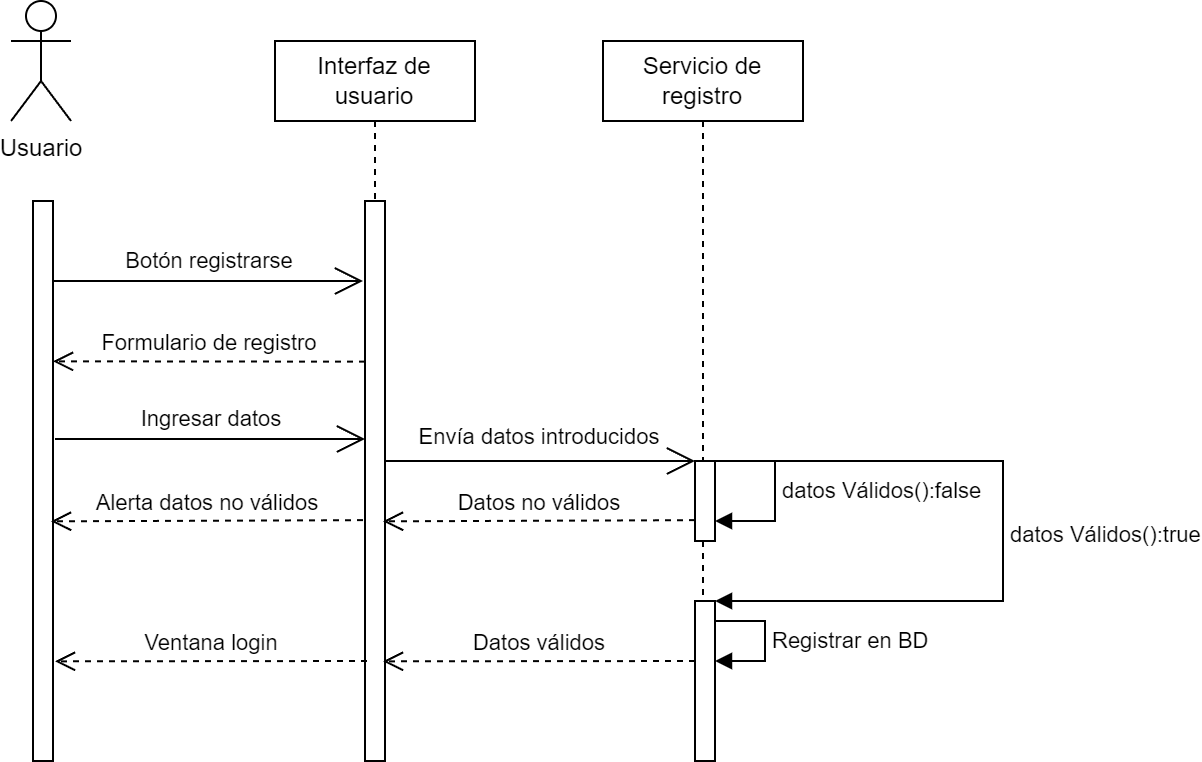
\includegraphics[width=1.0\textwidth]{diagrama-registro}
\caption{Diagrama de secuencia del registro.}
\label{fig:diagrama-secuencia-resgistro}
\end{figure}

\newpage
\subsection{Inicio sesión}
Se muestra el diagrama de secuencia en la ejecución del inicio de sesión.

\begin{figure}[!h]
\centering
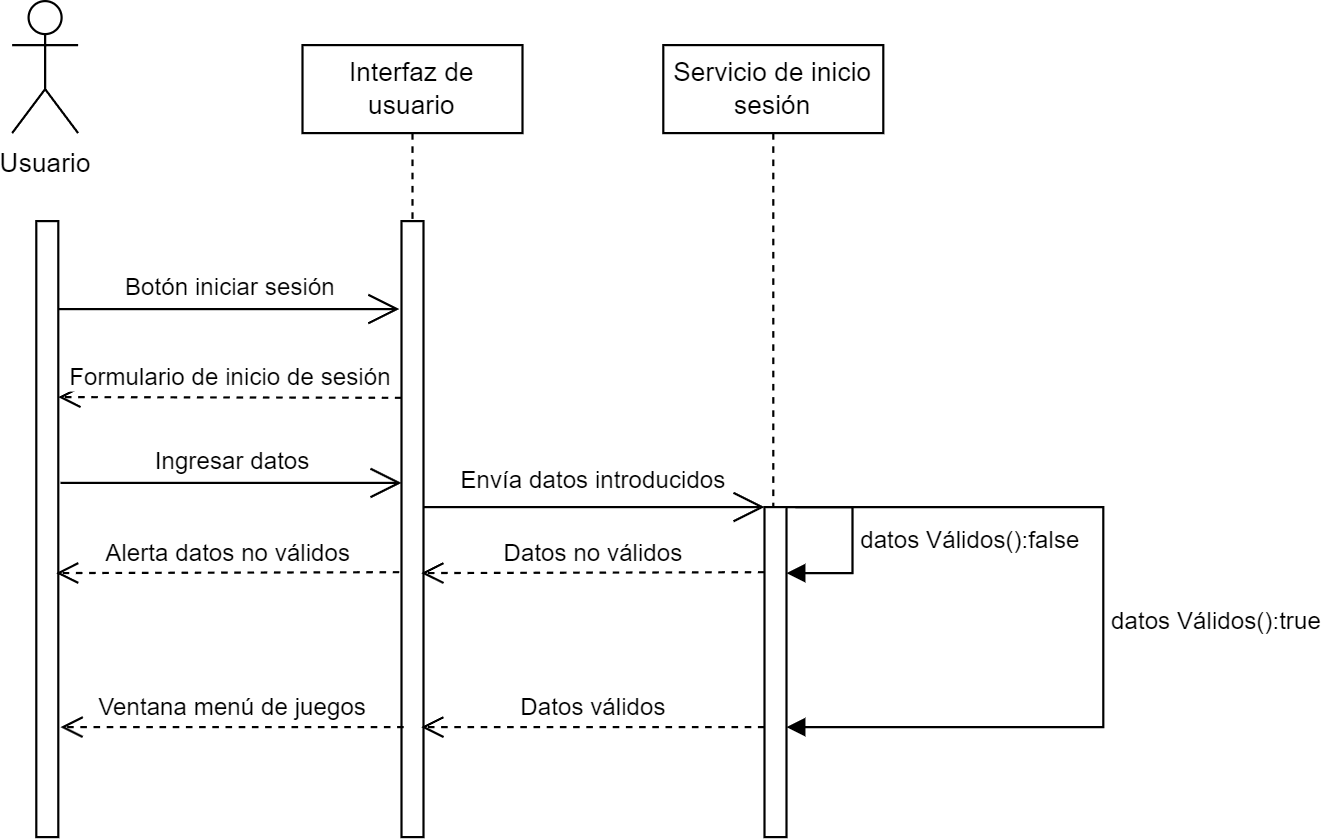
\includegraphics[width=1.0\textwidth]{diagrama-inicio}
\caption{Diagrama de secuencia del inicio de sesión.}
\label{fig:diagrama-secuencia-inicio-sesion}
\end{figure}

\newpage
\subsection{Visualización información de juego}
Se muestra el diagrama de secuencia en la ejecución de la visualización información de juego.
\begin{figure}[htb]
\centering
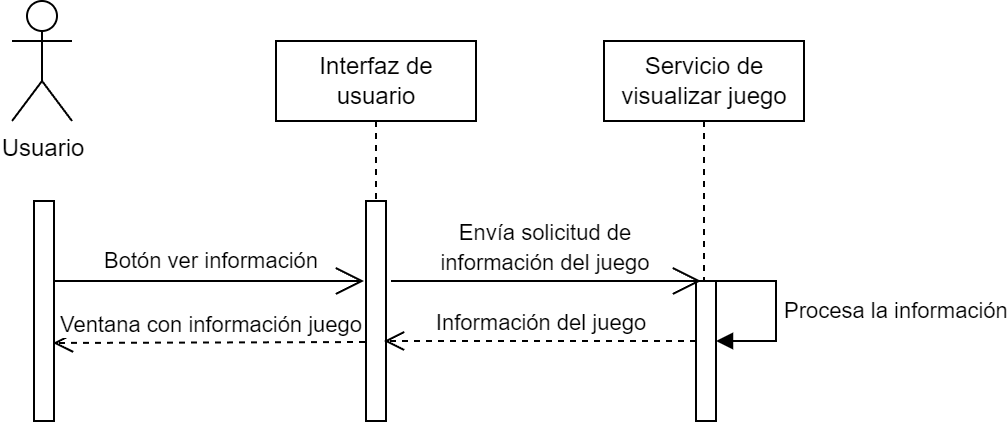
\includegraphics[width=0.9\textwidth]{diagrama-ver-juego}
\caption{Diagrama de secuencia del inicio de sesión.}
\label{fig:diagrama-secuencia-información-juego}
\end{figure}

\subsection{Visualización valoraciones de juego}
Se muestra el diagrama de secuencia en la ejecución de ver las valoraciones de un juego.
\begin{figure}[htb]
\centering
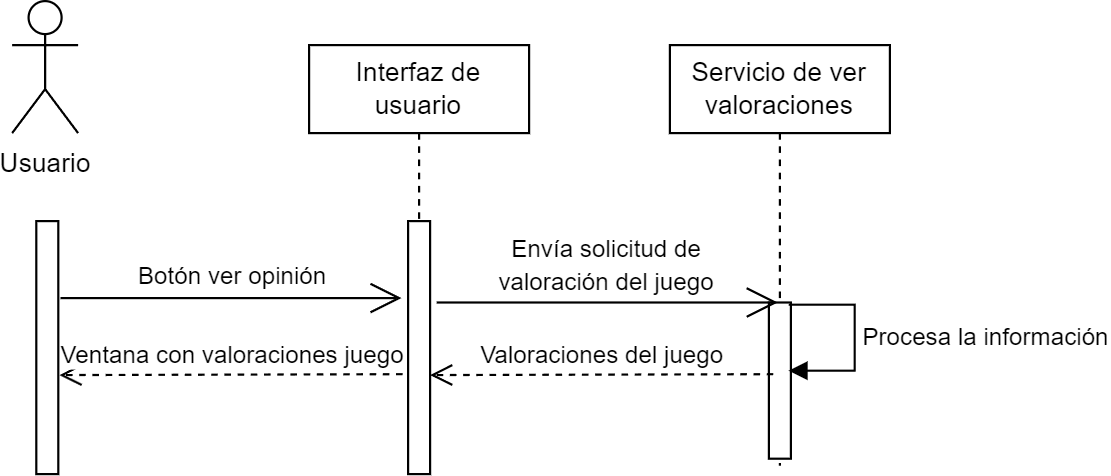
\includegraphics[width=1.0\textwidth]{diagrama-valoraciones}
\caption{Diagrama de secuencia de visualización de valoraciones.}
\label{fig:diagrama-secuencia-ver-valoraciones}
\end{figure}

\newpage
\subsection{Añadir valoración}
Se muestra el diagrama de secuencia en la ejecución de añadir una valoración a un juego.

\begin{figure}[htb]
\centering
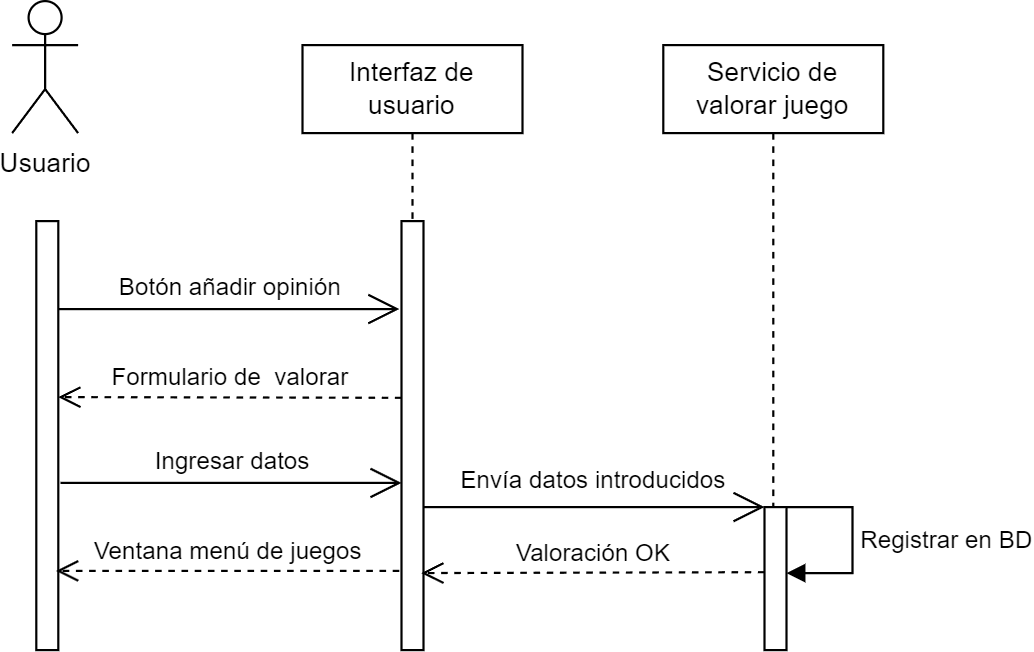
\includegraphics[width=1.0\textwidth]{diagrama-valorar-juego}
\caption{Diagrama de secuencia de añadir una valoración a un juego.}
\label{fig:diagrama-secuencia-añadir-valoración}
\end{figure}

\newpage
\subsection{Añadir juego}
Se muestra el diagrama de secuencia en la ejecución de añadir un nuevo juego.

\begin{figure}[h!]
\centering
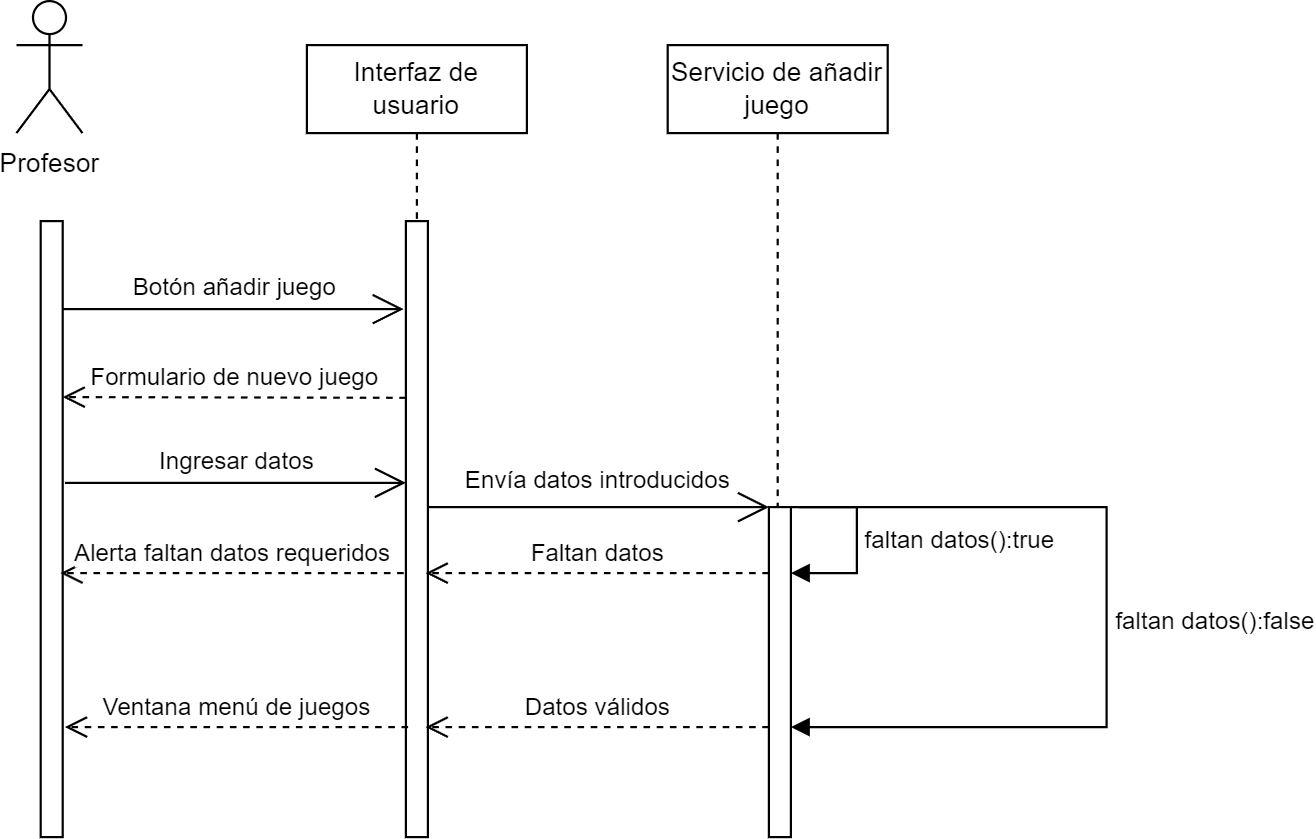
\includegraphics[width=1.0\textwidth]{diagrama-añadir-juego}
\caption{Diagrama de secuencia de añadir juego.}
\label{fig:diagrama-secuencia-añadir-juego}
\end{figure}

\newpage
\subsection{Modificar juego}
Se muestra el diagrama de secuencia en la ejecución de añadir un nuevo juego.

\begin{figure}[h!]
\centering
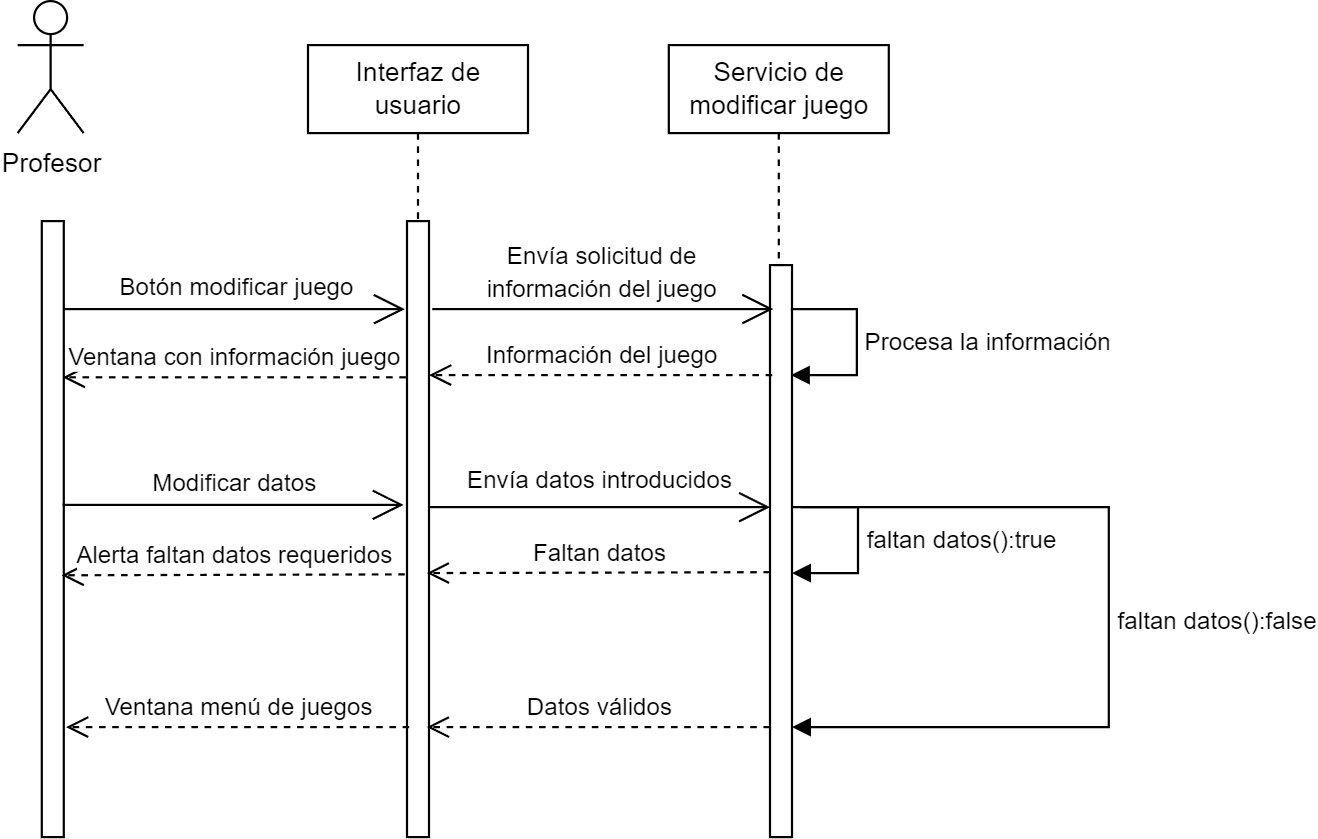
\includegraphics[width=1.0\textwidth]{diagrama-modificar-juego}
\caption{Diagrama de secuencia de modificar un juego.}
\label{fig:diagrama-secuencia-modificar-juego}
\end{figure}

\newpage
\subsection{Añadir archivos}
Se muestra el diagrama de secuencia en la ejecución de añadir archivos a la información del juego.

\begin{figure}[h!]
\centering
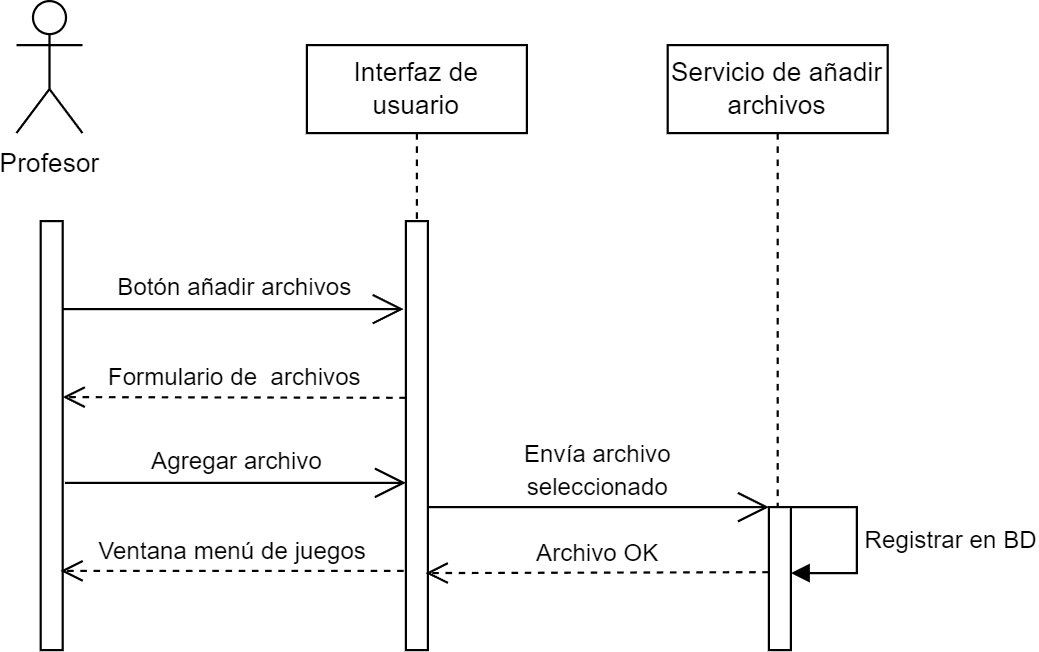
\includegraphics[width=1.0\textwidth]{diagrama-añadir-archivos}
\caption{Diagrama de secuencia de añadir archivos.}
\label{fig:diagrama-secuencia-añadir-archivos}
\end{figure}

\newpage
\subsection{Administración}
Se muestra el diagrama de secuencia en la ejecución de la administración.
\begin{figure}[h!]
\centering
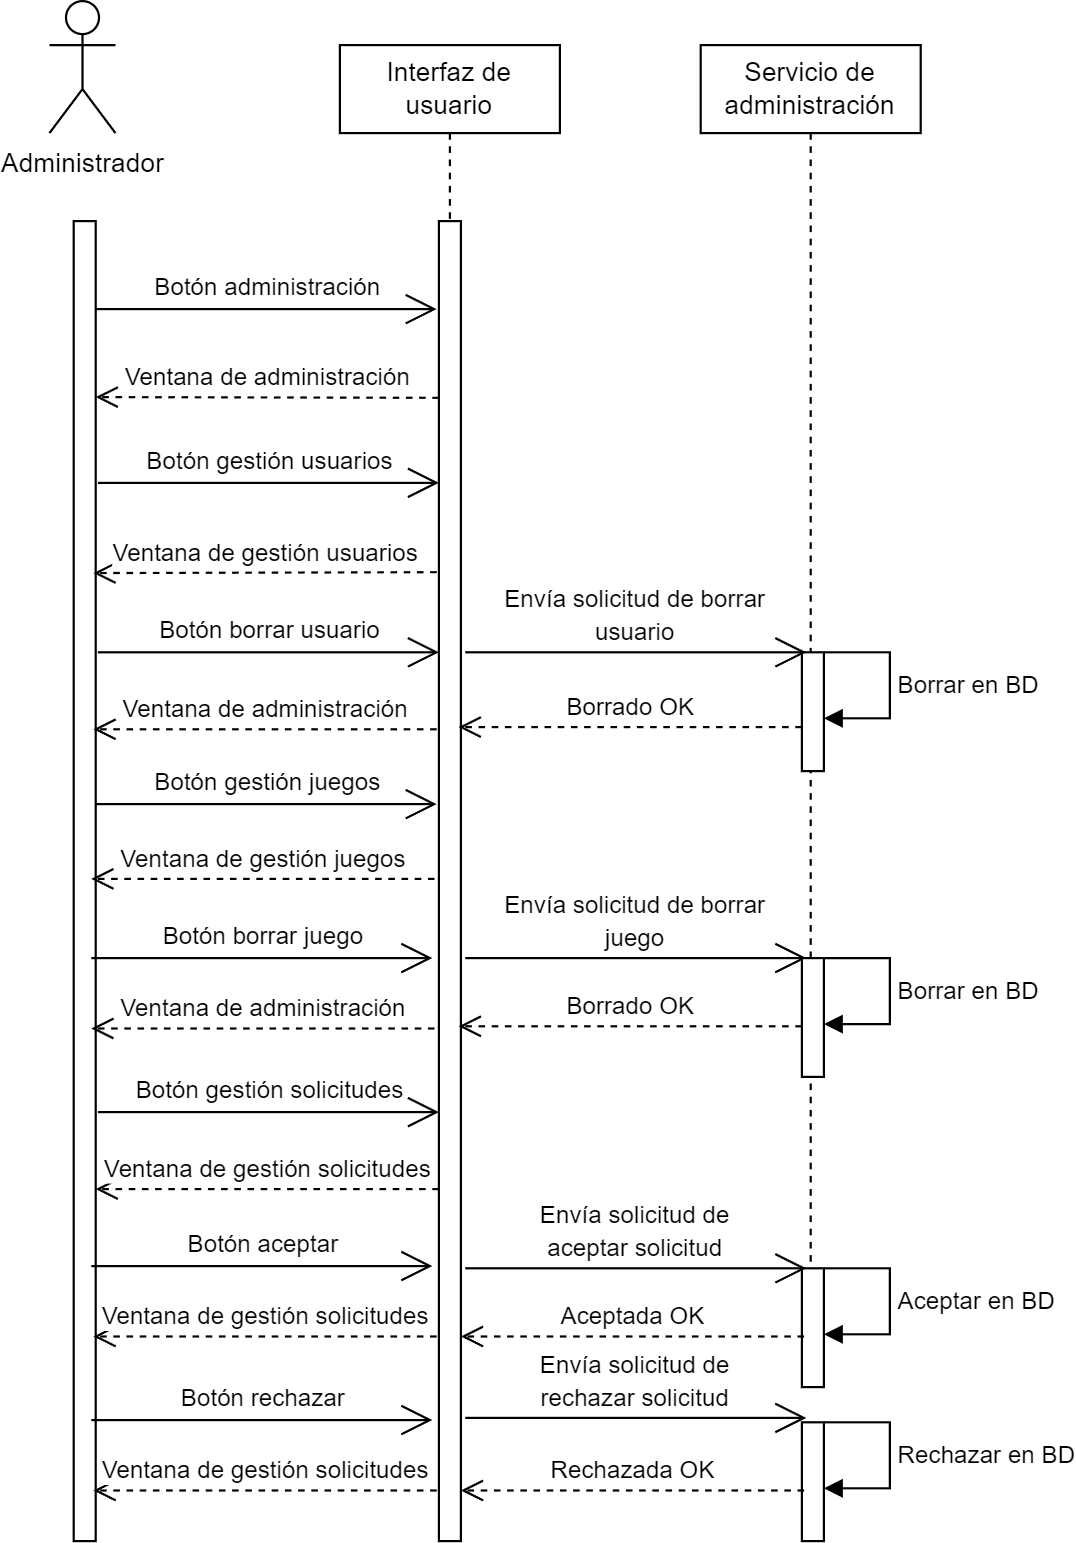
\includegraphics[width=0.8\textwidth]{diagrama-administracion}
\caption{Diagrama de secuencia de administración.}
\label{fig:diagrama-secuencia-administración}
\end{figure}

\newpage
\subsection{Modelo-Vista-Controlador (MVC)}
La arquitectura MVC, compuesta por el modelo, la vista y el controlador, separa los datos de la aplicación, la interfaz de usuario y la lógica de control.

En la aplicación, cada parte se atribuye de la siguiente manera:
\begin{itemize}
    \item\textbf{Modelo:} compuesto por los archivos database.py, juego.py, usuario.py, valoracion.py y solicitud.py. Estos archivos interactúan con la base de datos, realizando operaciones de creación, lectura, actualización y eliminación de los datos.
    \item\textbf{Vista:} compuesta por los templates HTML que presentan la visualización de las interfaces de usuario.
    \item\textbf{Controlador:} compuesto por el archivo app.py, ya que se encarga de la comunicación con los servicios de la vista. Maneja la interacción entre el modelo y la vista, devolviendo la información deseada.
\end{itemize}

\subsection{Fachada}
El patrón Fachada es un diseño estructural que proporciona una interfaz simplificada y unificada al cliente. Este patrón se emplea para simplificar la interacción del usuario con un subsistema más grande y complejo, como los módulos que se encargan de las operaciones en la base de datos en nuestra aplicación. En este sentido, el módulo app.py cumple el rol de fachada, ya que se encarga de comunicar los demás módulos con el cliente, proporcionando una interfaz coherente y simplificada.


\section{Diseño de interfaces}
Para la realización del proyecto se desarrolló el prototipo de las interfaces de la aplicación web mediante el uso de la herramienta de diseño Figma, con el fin de establecer inicialmente cómo iba a ser la aplicación web.

\subsection{Inicio}
La primera interfaz que se diseñó fue el prototipo de la página principal de inicio de la aplicación. Esta interfaz permite a los usuarios registrarse, iniciar sesión y comenzar a utilizar el repositorio de juegos, así como acceder a otras funcionalidades. Dependiendo del tipo de inicio de sesión (usuario, profesor o administrador), se les permitirá realizar diferentes acciones y acceder a diferentes funcionalidades.

\begin{figure}[htb]
\centering
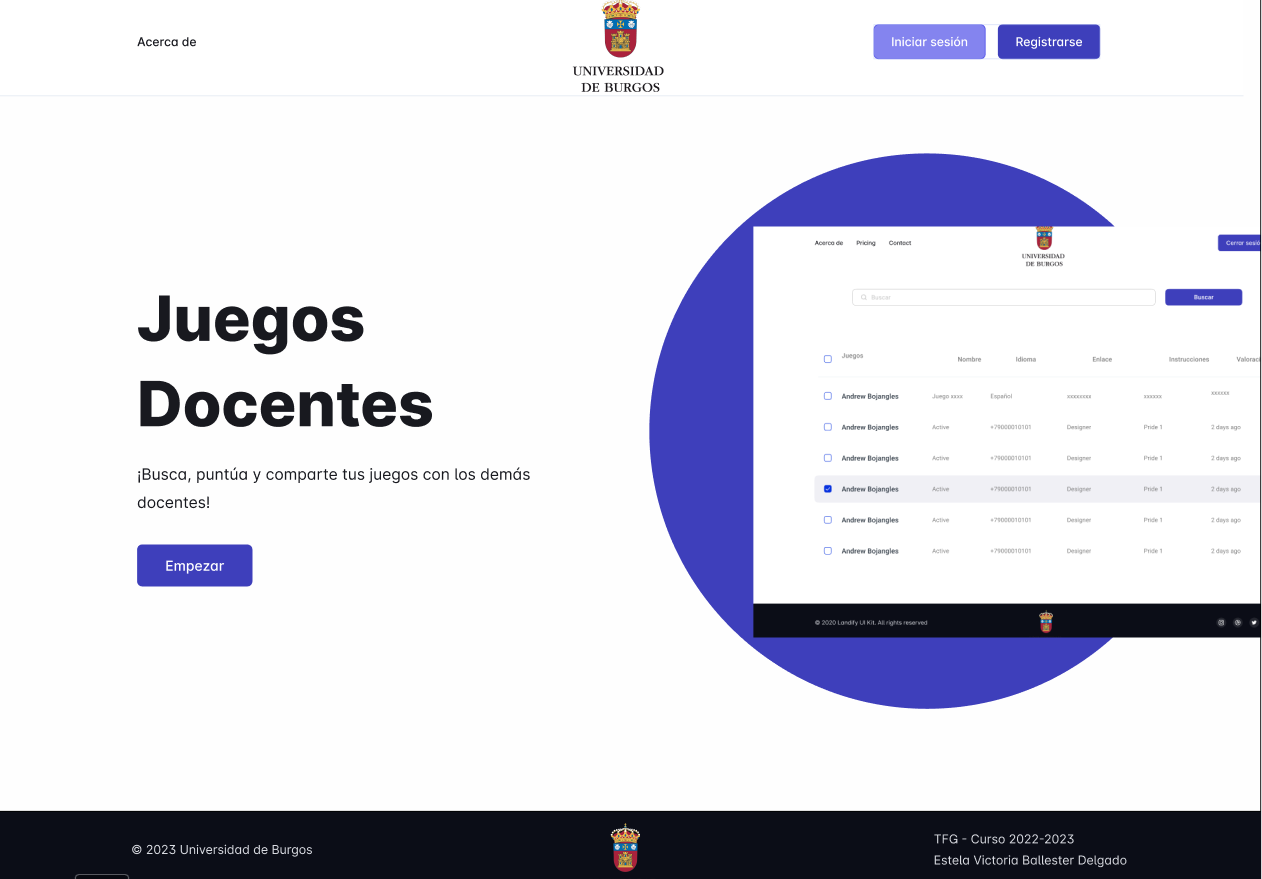
\includegraphics[width=0.7\textwidth]{inicio-prototipo}
\caption{Prototipo del inicio.}
\label{fig:inicio-prototipo}
\end{figure}

Finalmente, el resultado del template inicio.html quedó de la siguiente manera:

\begin{figure}[htb]
\centering
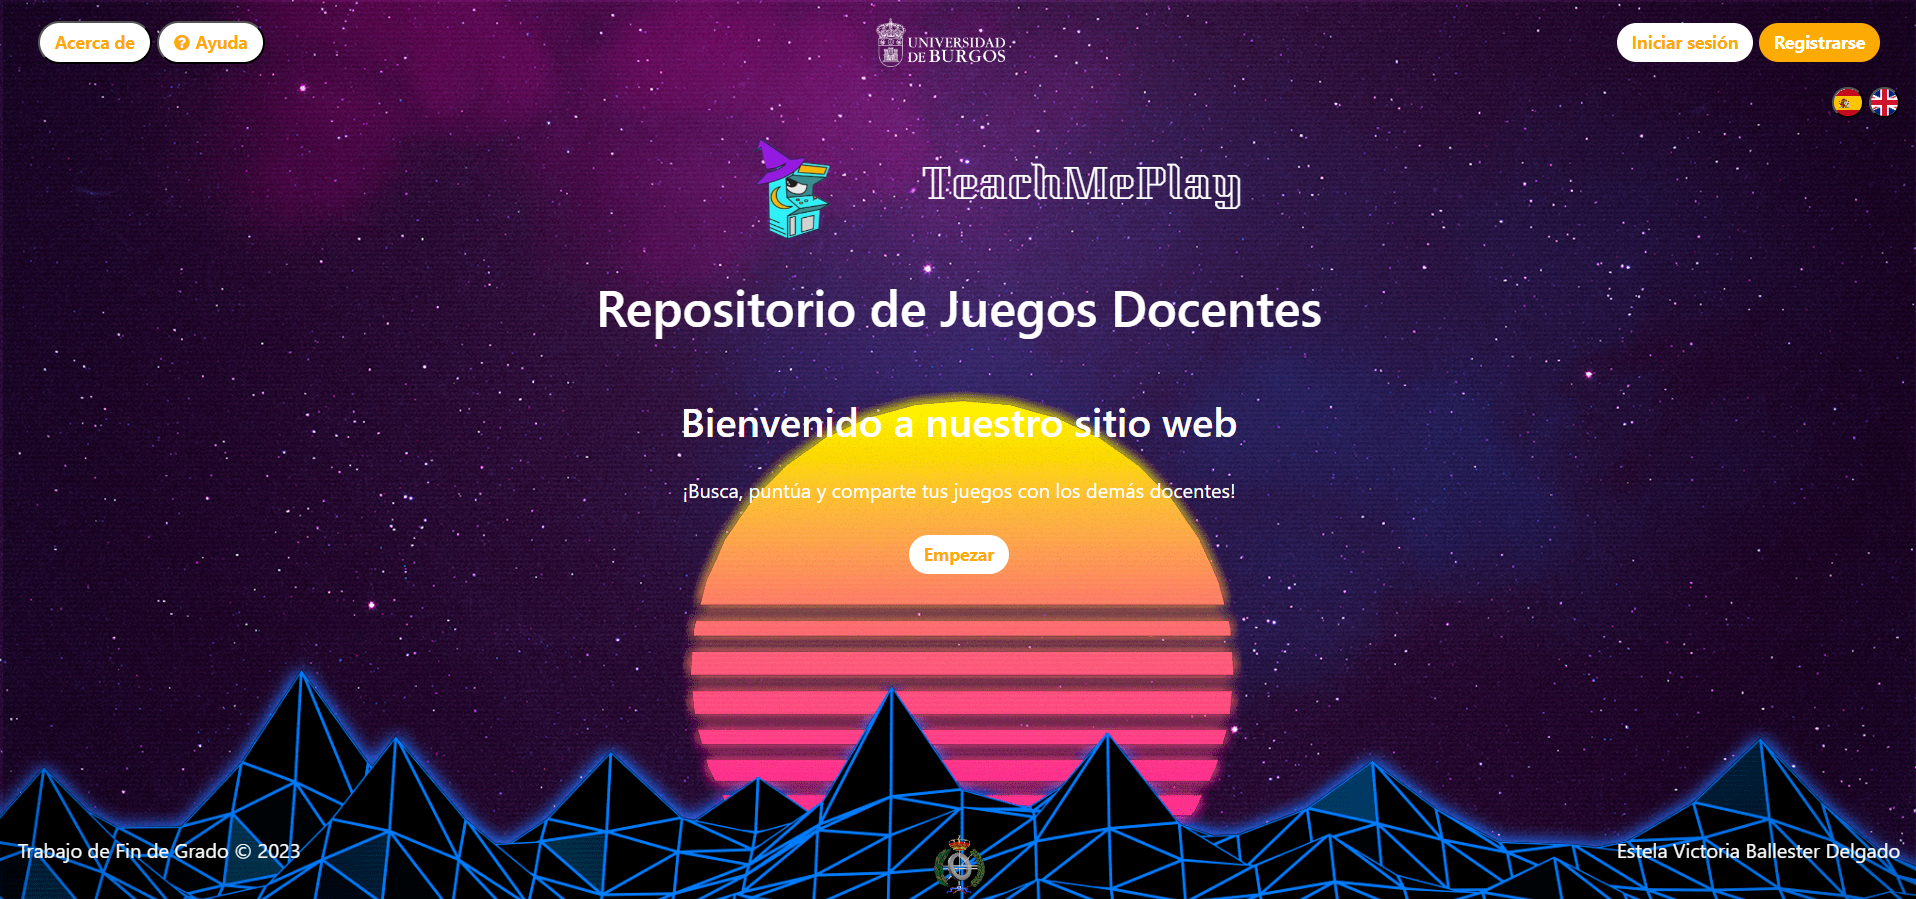
\includegraphics[width=0.8\textwidth]{inicio}
\caption{Interfaz del inicio.}
\label{fig:inicio}
\end{figure}

Como se puede apreciar, el resultado final del template inicio.html es prácticamente idéntico al prototipo en cuanto a funcionalidad. El diseño y la disposición de los elementos no se han mantenido tan fieles a la idea inicial, pero se refleja una buena implementación y una coherencia visual en la aplicación.

\subsection{Registro}
La interfaz de registro solicita al usuario introducir una serie de campos obligatorios entre los que se incluyen el nombre, la universidad y la contraseña. En el caso de tener ya una cuenta permite iniciar sesión desde ahí.

\begin{figure}[htb]
\centering
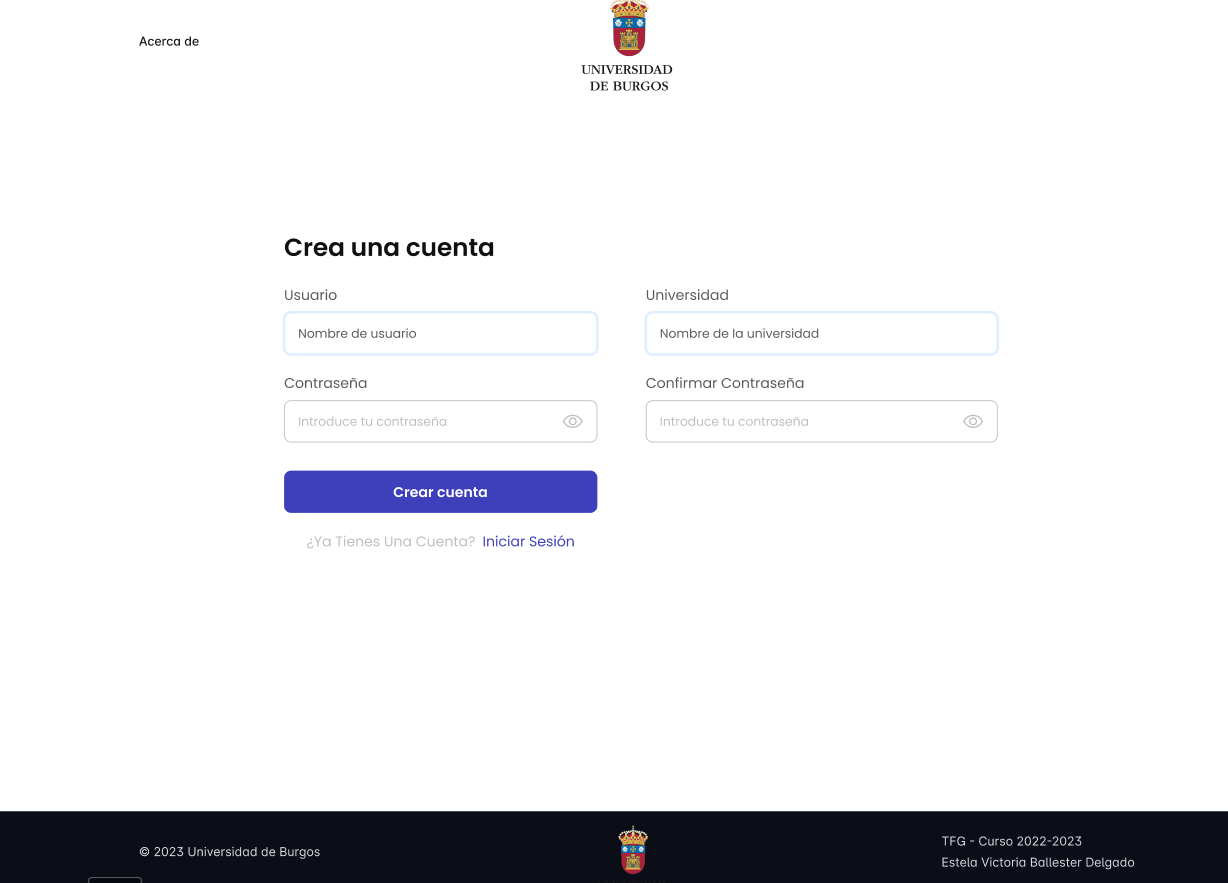
\includegraphics[width=0.7\textwidth]{registro-prototipo}
\caption{Prototipo del registro.}
\label{fig:registro-prototipo}
\end{figure}

Finalmente, el resultado del template registro.html quedó de la siguiente manera:

\begin{figure}[htb]
\centering
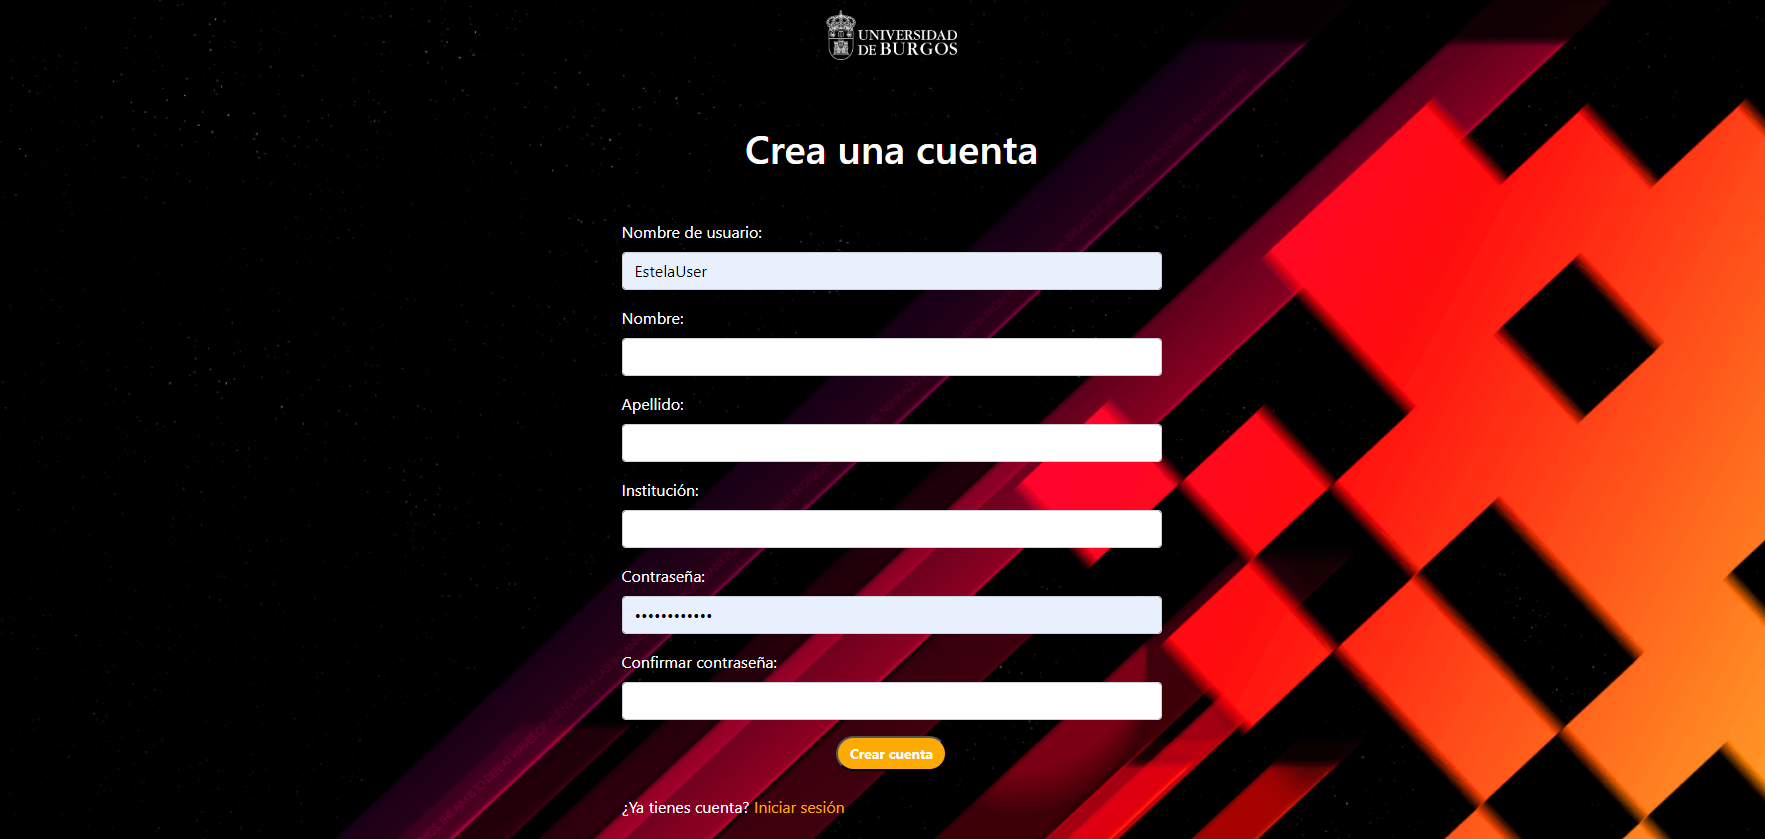
\includegraphics[width=0.8\textwidth]{registro}
\caption{Interfaz del registro.}
\label{fig:registro}
\end{figure}

Como se puede observar, el resultado final del template registro.html es prácticamente idéntico al prototipo inicial. Sin embargo, se han realizado algunas modificaciones para mejorar la funcionalidad del formulario de registro. En particular, se han agregado campos obligatorios adicionales, como el nombre y apellido del usuario, con el fin de recopilar información más completa durante el proceso de registro.

\subsection{Inicio de sesión}
La interfaz de inicio de sesión solicita al usuario introducir su nombre de usuario y la contraseña de su cuenta. También permite registrarse en el caso de no tener una cuenta creada. Además ofrece la posibilidad de recordar la contraseña si el usuario no la recuerda.

\begin{figure}[htb]
\centering
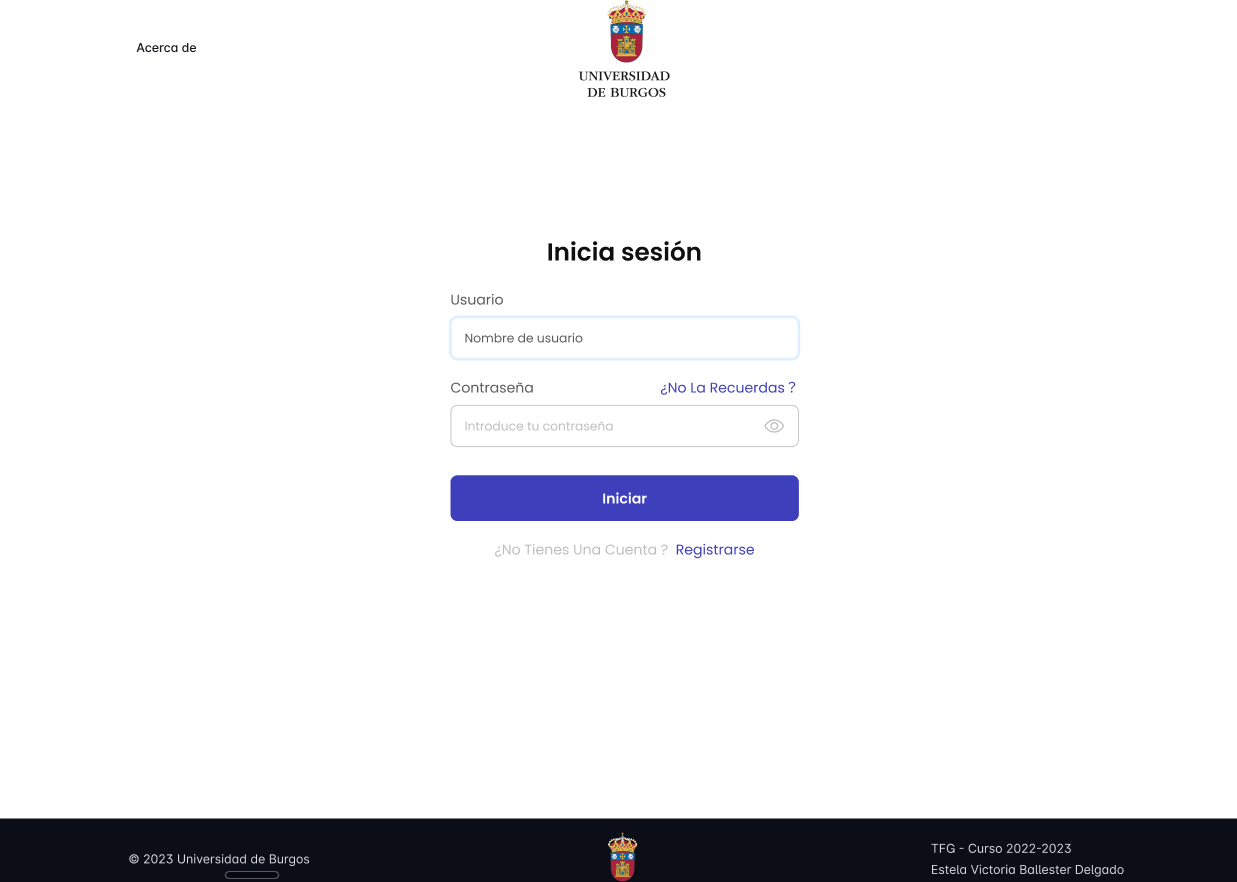
\includegraphics[width=0.7\textwidth]{login-prototipo}
\caption{Prototipo del inicio de sesión.}
\label{fig:login-prototipo}
\end{figure}

Finalmente, el resultado del template login.html quedó de la siguiente manera:
\newpage
\begin{figure}[htb]
\centering
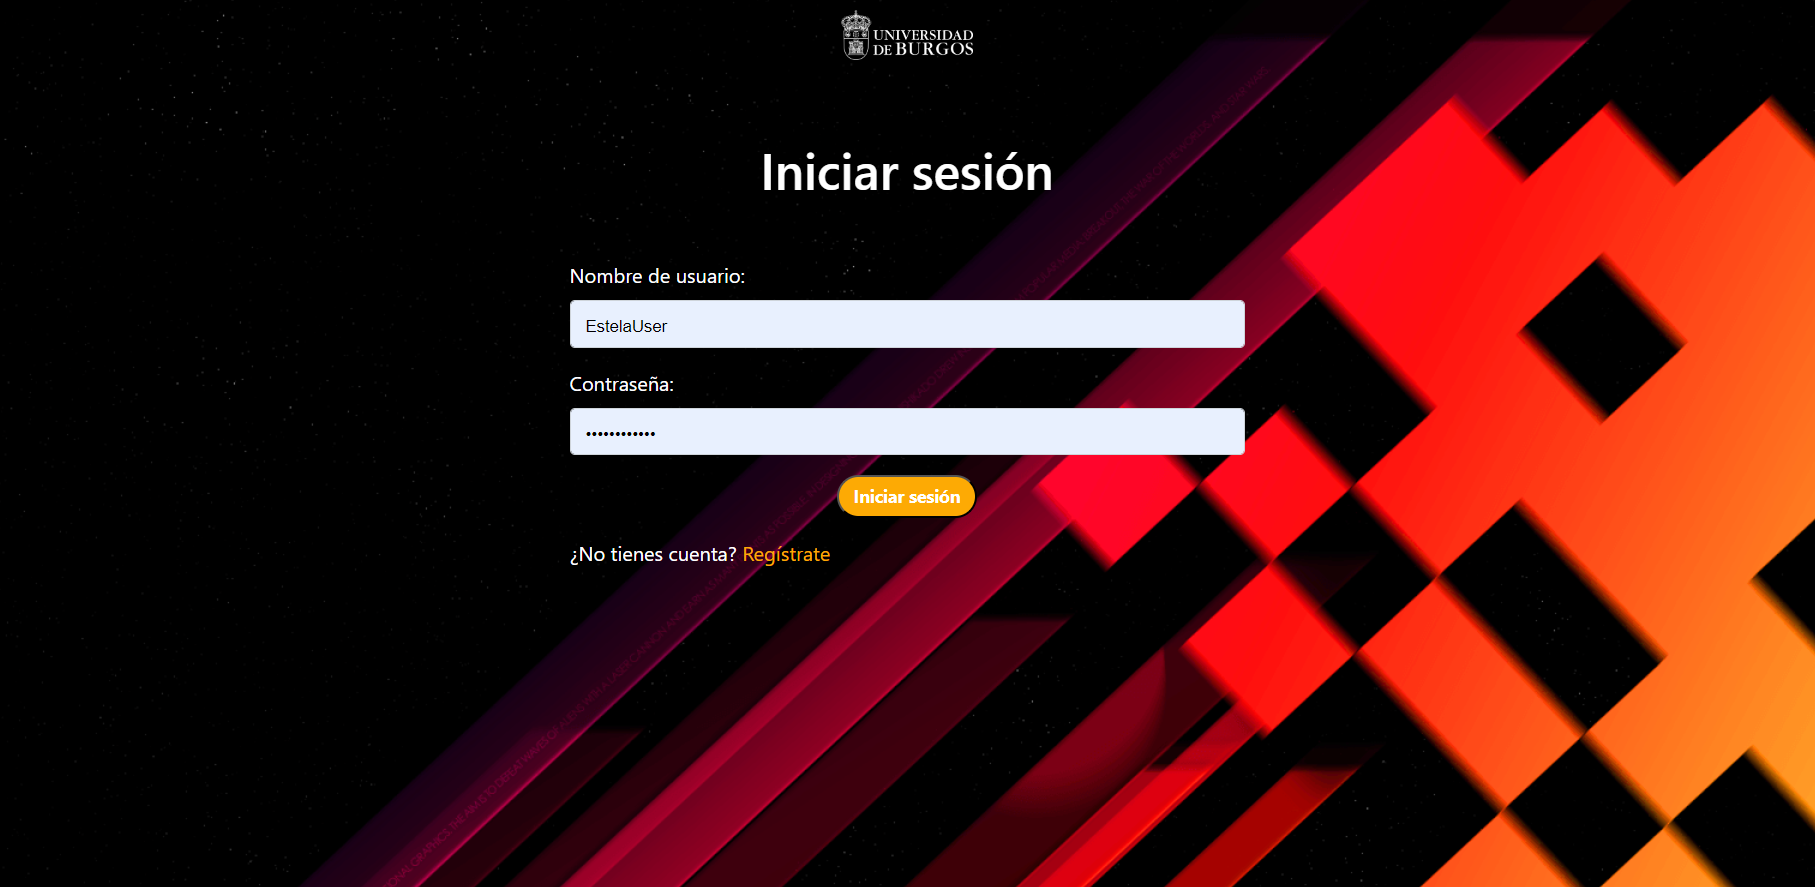
\includegraphics[width=0.8\textwidth]{login}
\caption{Interfaz del inicio de sesión.}
\label{fig:login}
\end{figure}

Como se puede observar, el resultado final del template login.html es prácticamente idéntico al prototipo inicial. Sin embargo, se diferencia en que finalmente no se implementó la funcionalidad de recuperación de contraseña en caso de olvido. Esta decisión se tomó con el objetivo de simplificar el proceso de inicio de sesión y priorizar otras funcionalidades importantes

\subsection{Menú de juegos de usuarios}
La interfaz del menú de juegos de los usuarios permite realizar búsquedas personalizadas de los juegos, visualizar la información detallada de cada juego y además brinda la opción de valorarlos.

\begin{figure}[htb]
\centering
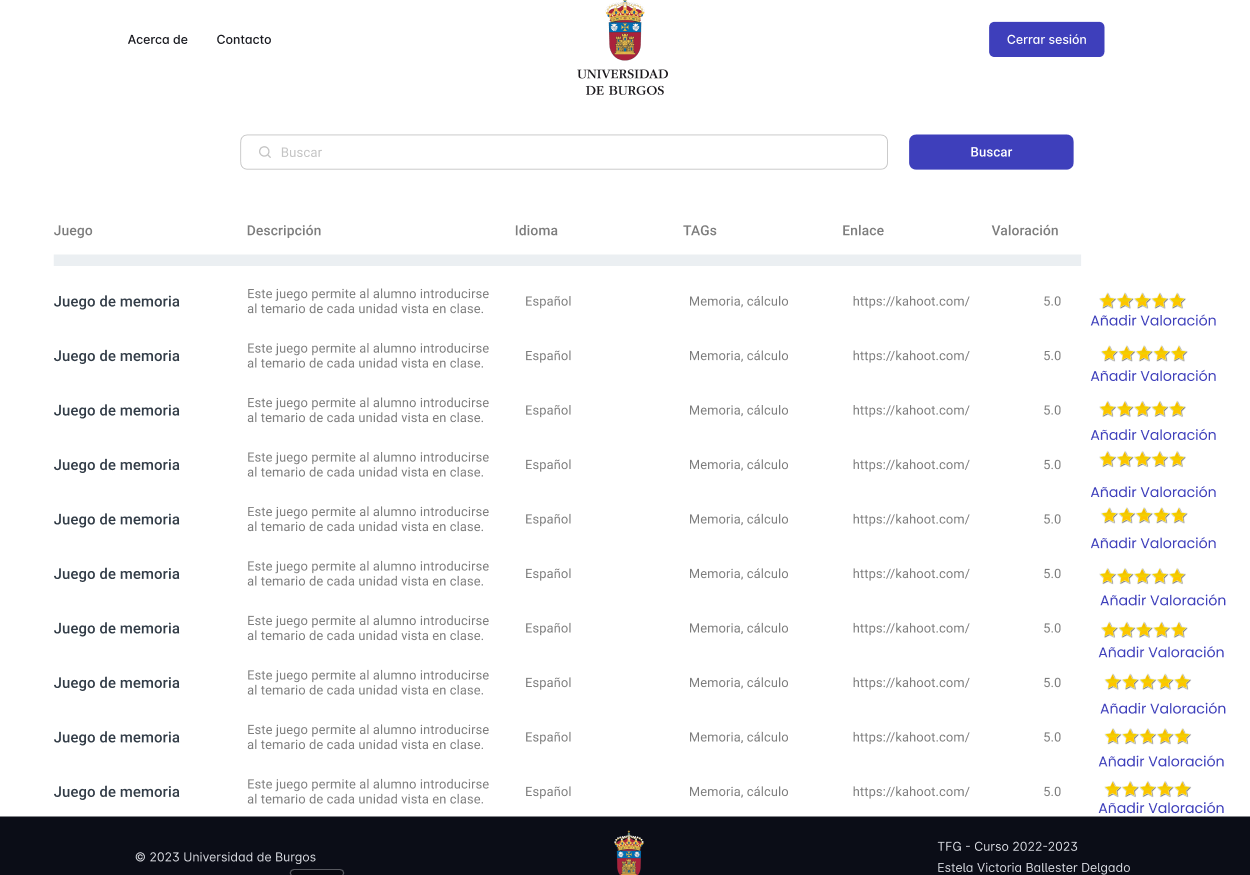
\includegraphics[width=0.7\textwidth]{menu-usuarios-prototipo}
\caption{Prototipo del menú de juegos de usuarios.}
\label{fig:menu-usuarios-prototipo}
\end{figure}

\newpage
Finalmente, el resultado del template menu\_juegos\_usuario.html quedó de la siguiente manera:

\begin{figure}[htb]
\centering
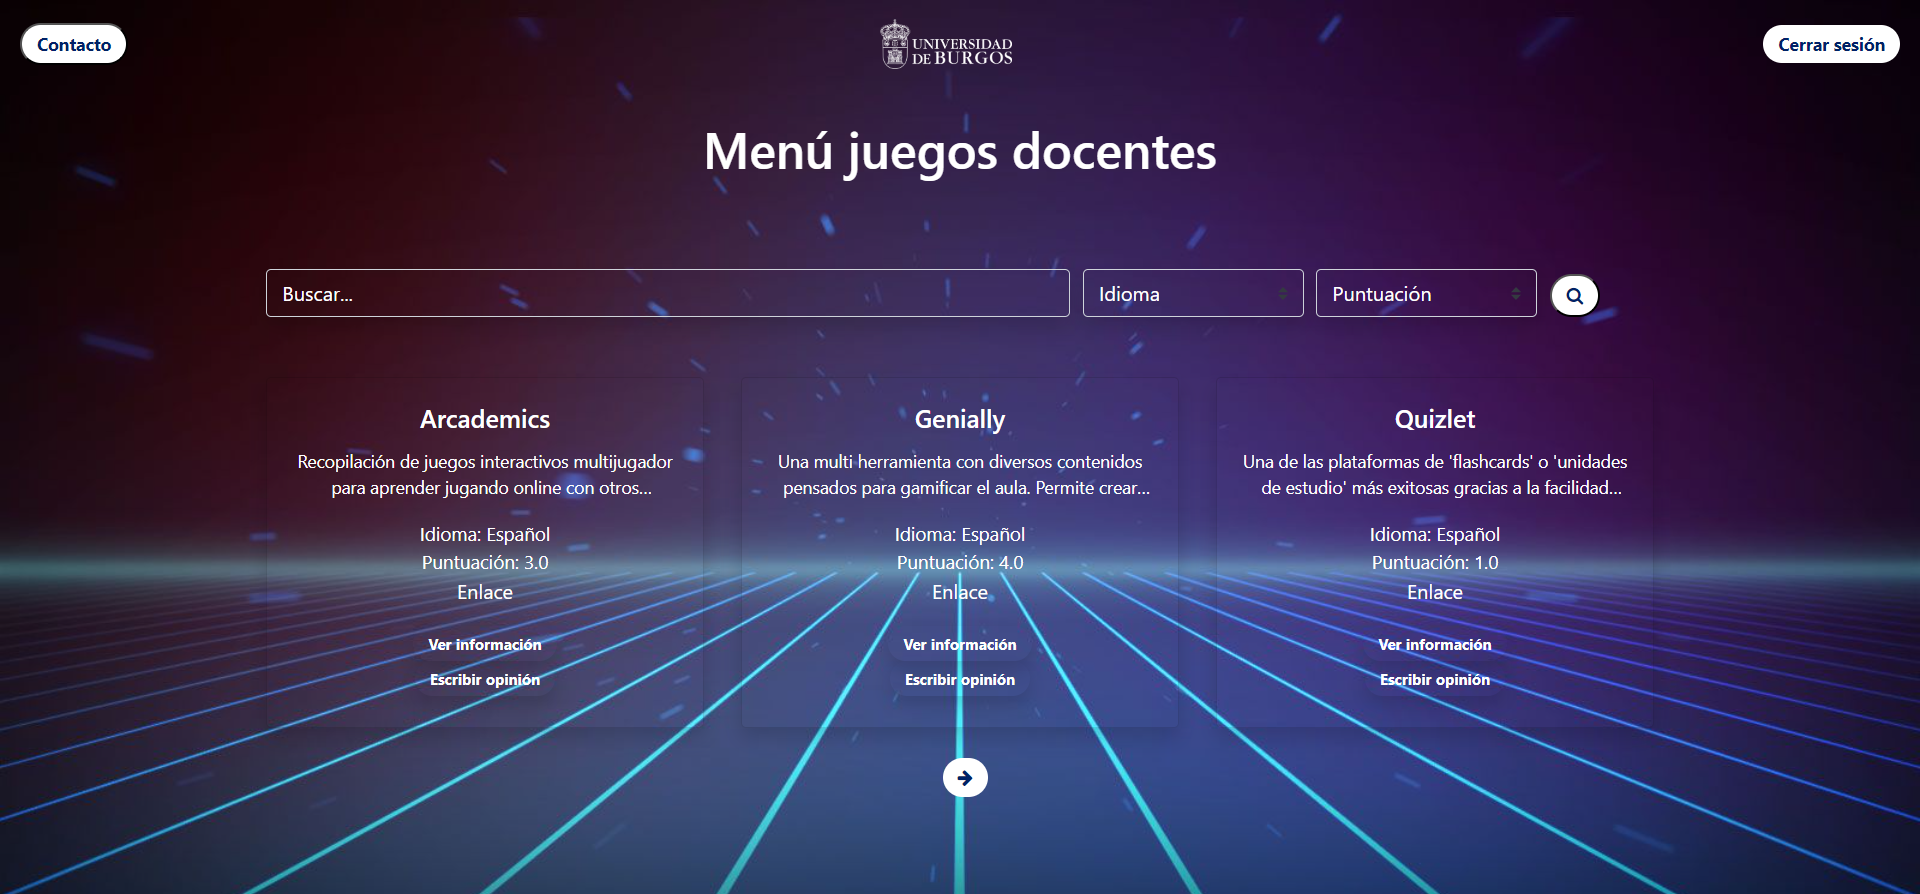
\includegraphics[width=0.7\textwidth]{menu-usuarios}
\caption{Interfaz del menú de juegos de usuarios.}
\label{fig:menu-usuarios}
\end{figure}

Como se puede observar, el resultado final del template menu\_juegos\_usuario.html presenta varias diferencias visuales en comparación con el prototipo inicial. La principal diferencia radica en la forma en que se muestran los juegos, ya que en el prototipo se mostraban en forma de tabla y en el resultado final se presentan en tarjetas, lo cual facilita su visualización. Además, en el resultado final se ha agregado la funcionalidad de realizar búsquedas utilizando tanto la barra de búsqueda como filtros, lo cual permite realizar búsquedas más específicas.

\subsection{Añadir valoración}
La interfaz de añadir una valoración a un juego permite introducir una puntuación y añadir un comentario escrito.

\begin{figure}[htb]
\centering
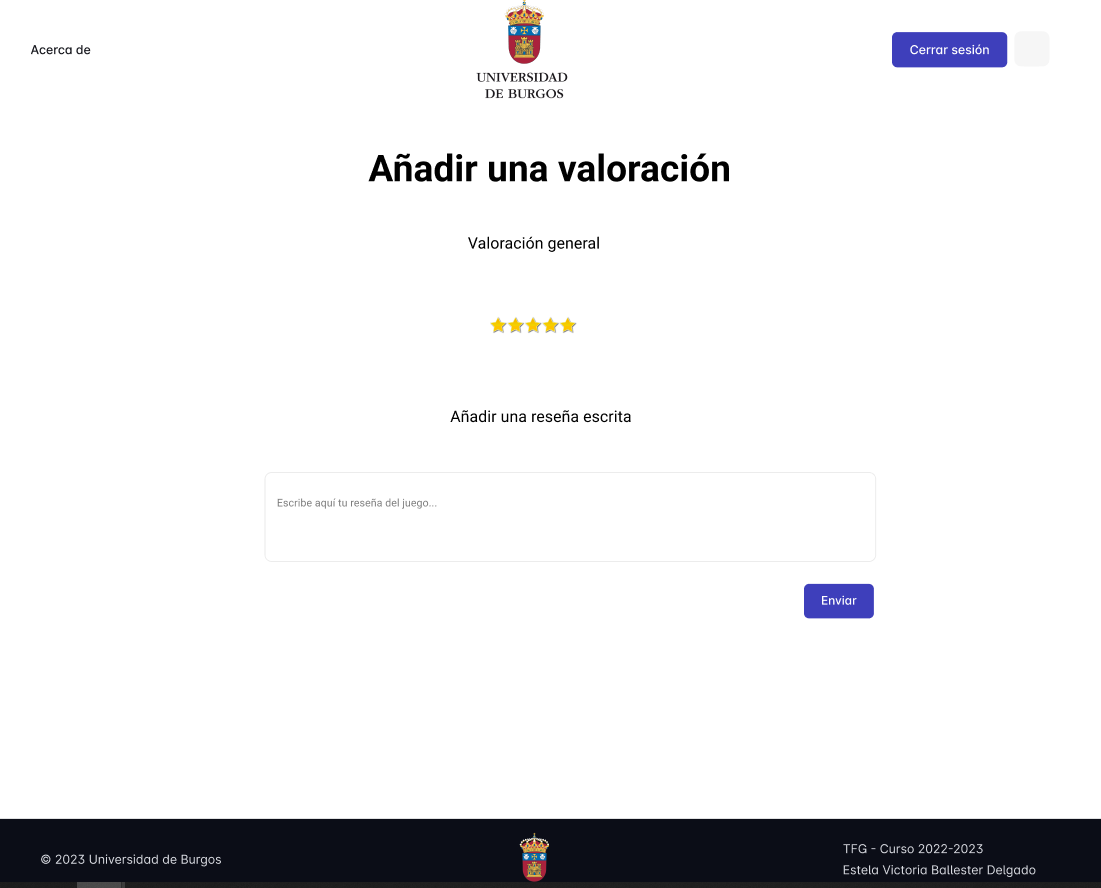
\includegraphics[width=0.7\textwidth]{añadir-valoracion-prototipo}
\caption{Prototipo de añadir una valoración.}
\label{fig:añadir-valoracion-prototipo}
\end{figure}

Finalmente, el resultado del template añadir\_valoracion.html quedó de la siguiente manera:

\begin{figure}[htb]
\centering
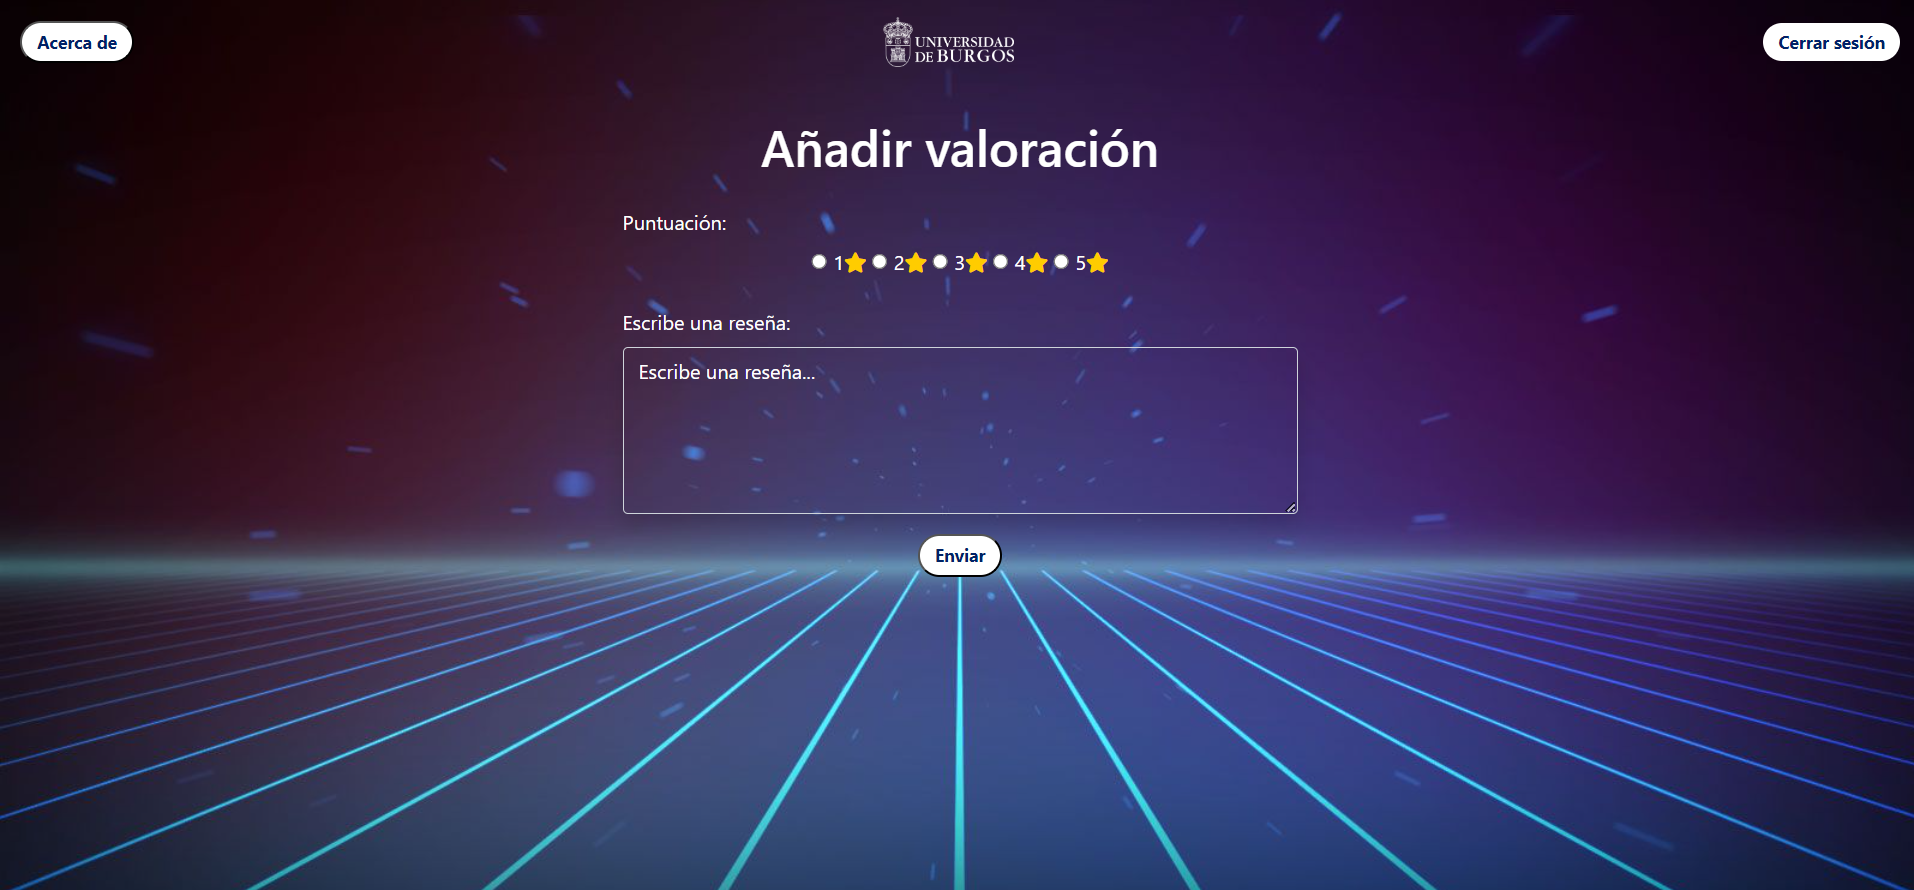
\includegraphics[width=0.8\textwidth]{añadir-valoracion}
\caption{Interfaz de añadir una valoración.}
\label{fig:añadir-valoracion}
\end{figure}

Como se puede observar, el resultado final del template añadir\_valoracion.html es prácticamente idéntico al prototipo inicial.

\subsection{Visualizar valoración}
La interfaz de visualizar las valoraciones de un juego permite ver todas las reseñas que han dejado los usuarios sobre dicho juego.

\begin{figure}[htb]
\centering
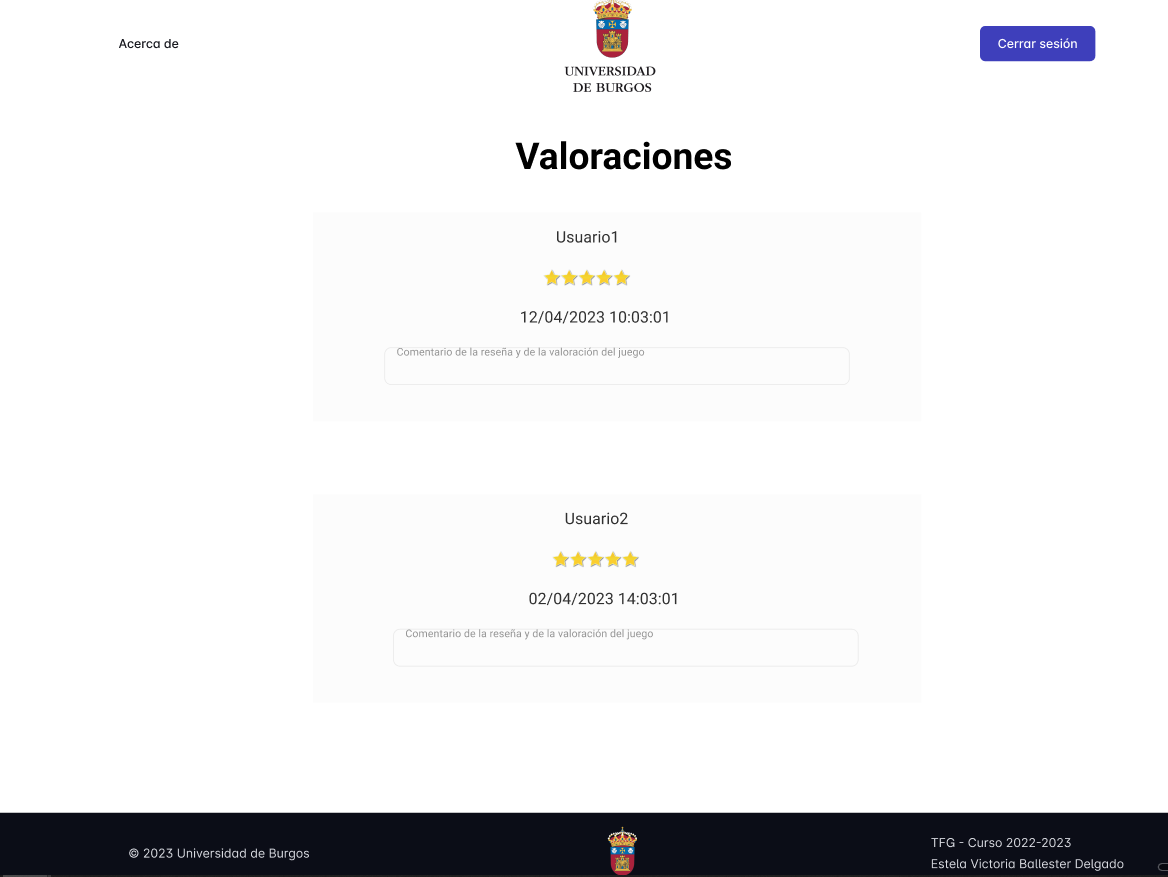
\includegraphics[width=0.7\textwidth]{visualizar-valoracion-prototipo}
\caption{Prototipo de la visualización de valoraciones.}
\label{fig:visualizar-valoracion-prototipo}
\end{figure}

Finalmente, el resultado del template visualizar\_valoracion.html quedó de la siguiente manera:

\begin{figure}[htb]
\centering
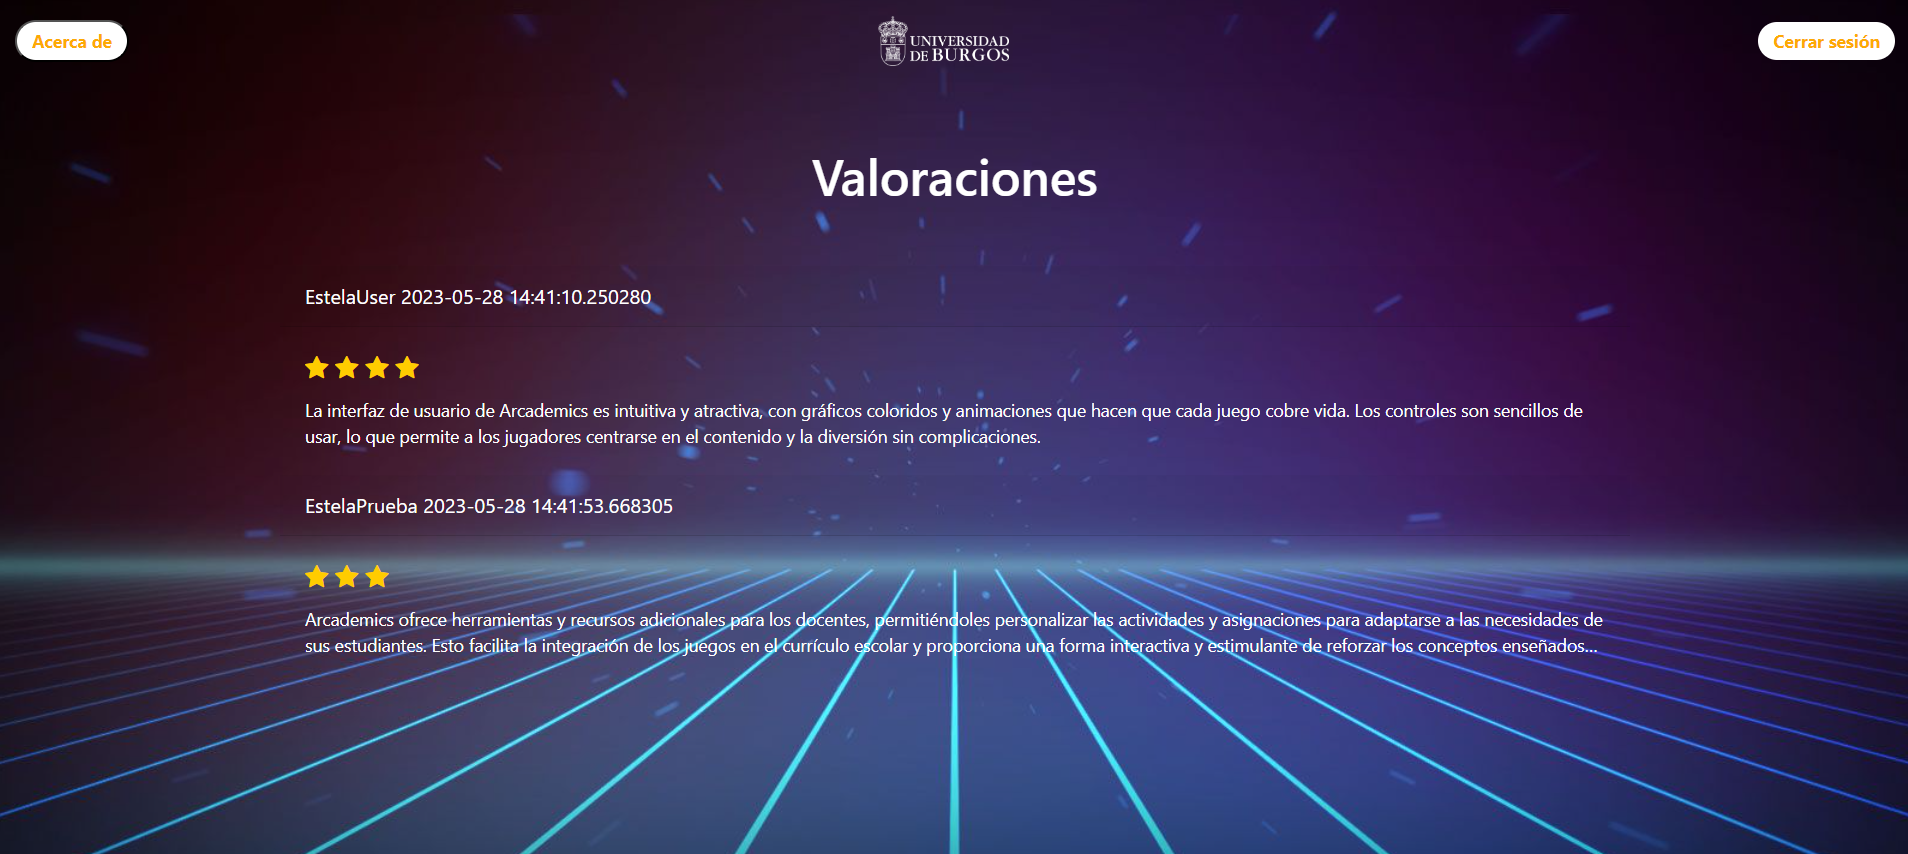
\includegraphics[width=0.8\textwidth]{visualizar-valoracion}
\caption{Interfaz de la visualización de valoraciones.}
\label{fig:visualizar-valoracion}
\end{figure}

Como se puede observar, el resultado final del template visualizar\_valoracion.html es prácticamente idéntico al prototipo inicial.

\subsection{Contacto}
La interfaz de contacto solo es accesible por los usuarios. Esta les permite solicitar el rol de profesor.

\begin{figure}[htb]
\centering

\includegraphics[width=0.7\textwidth]{solicitar}
\caption{Prototipo del contacto.}
\label{fig:solicitar}
\end{figure}

Finalmente, el resultado del template contacto.html quedó de la siguiente manera:

\begin{figure}[htb]
\centering
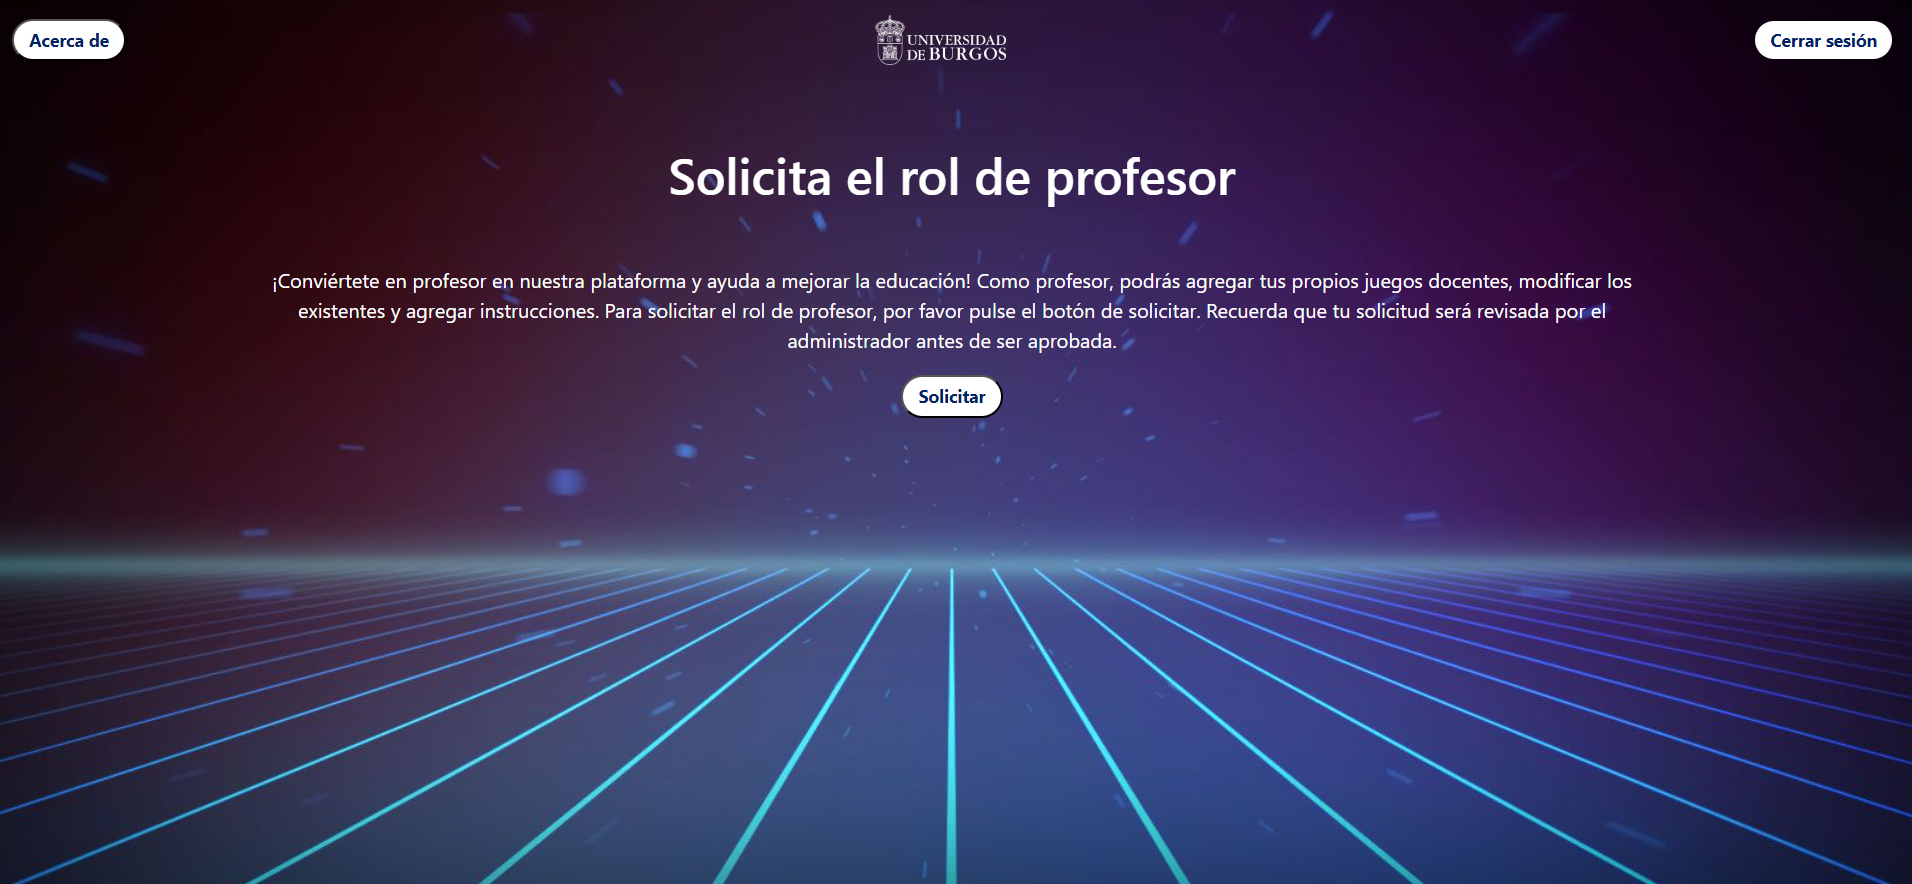
\includegraphics[width=0.8\textwidth]{contacto}
\caption{Interfaz del contacto.}
\label{fig:contacto}
\end{figure}

Como se puede observar, el resultado final del template contacto.html es prácticamente idéntico al prototipo inicial. 

\subsection{Menú de juegos de profesores}
La interfaz del menú de juegos de los profesores proporciona diversas funcionalidades. Permite realizar búsquedas personalizadas de los juegos, visualizar información detallada de cada juego, así como añadir nuevos juegos y modificar los existentes.

\begin{figure}[htb]
\centering
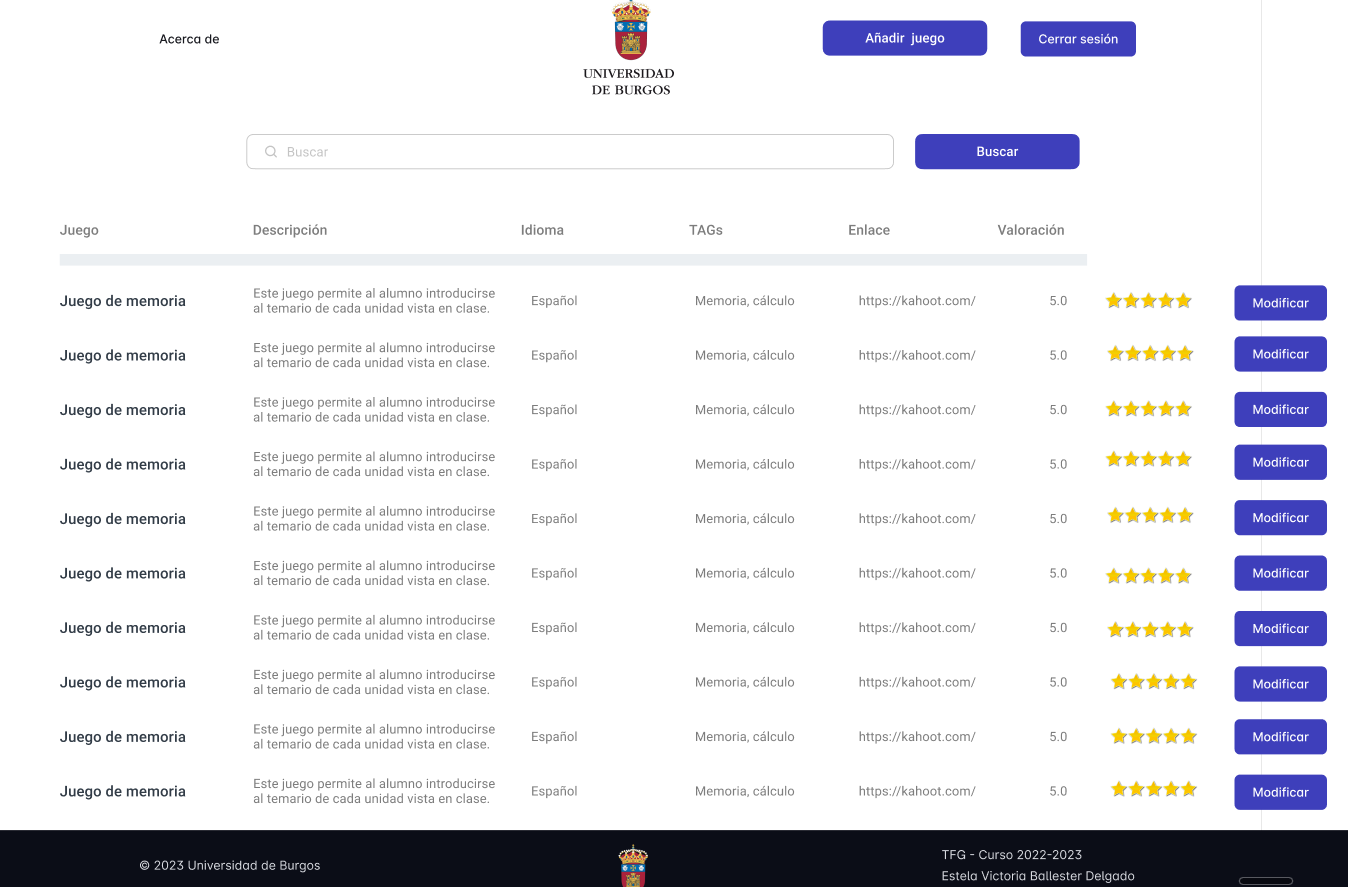
\includegraphics[width=0.7\textwidth]{menu-profesor-prototipo}
\caption{Prototipo del menú de juegos de profesores.}
\label{fig:menu-profesor-prototipo}
\end{figure}

Finalmente, el resultado del template menu\_juegos\_profesor.html quedó de la siguiente manera:

\begin{figure}[htb]
\centering
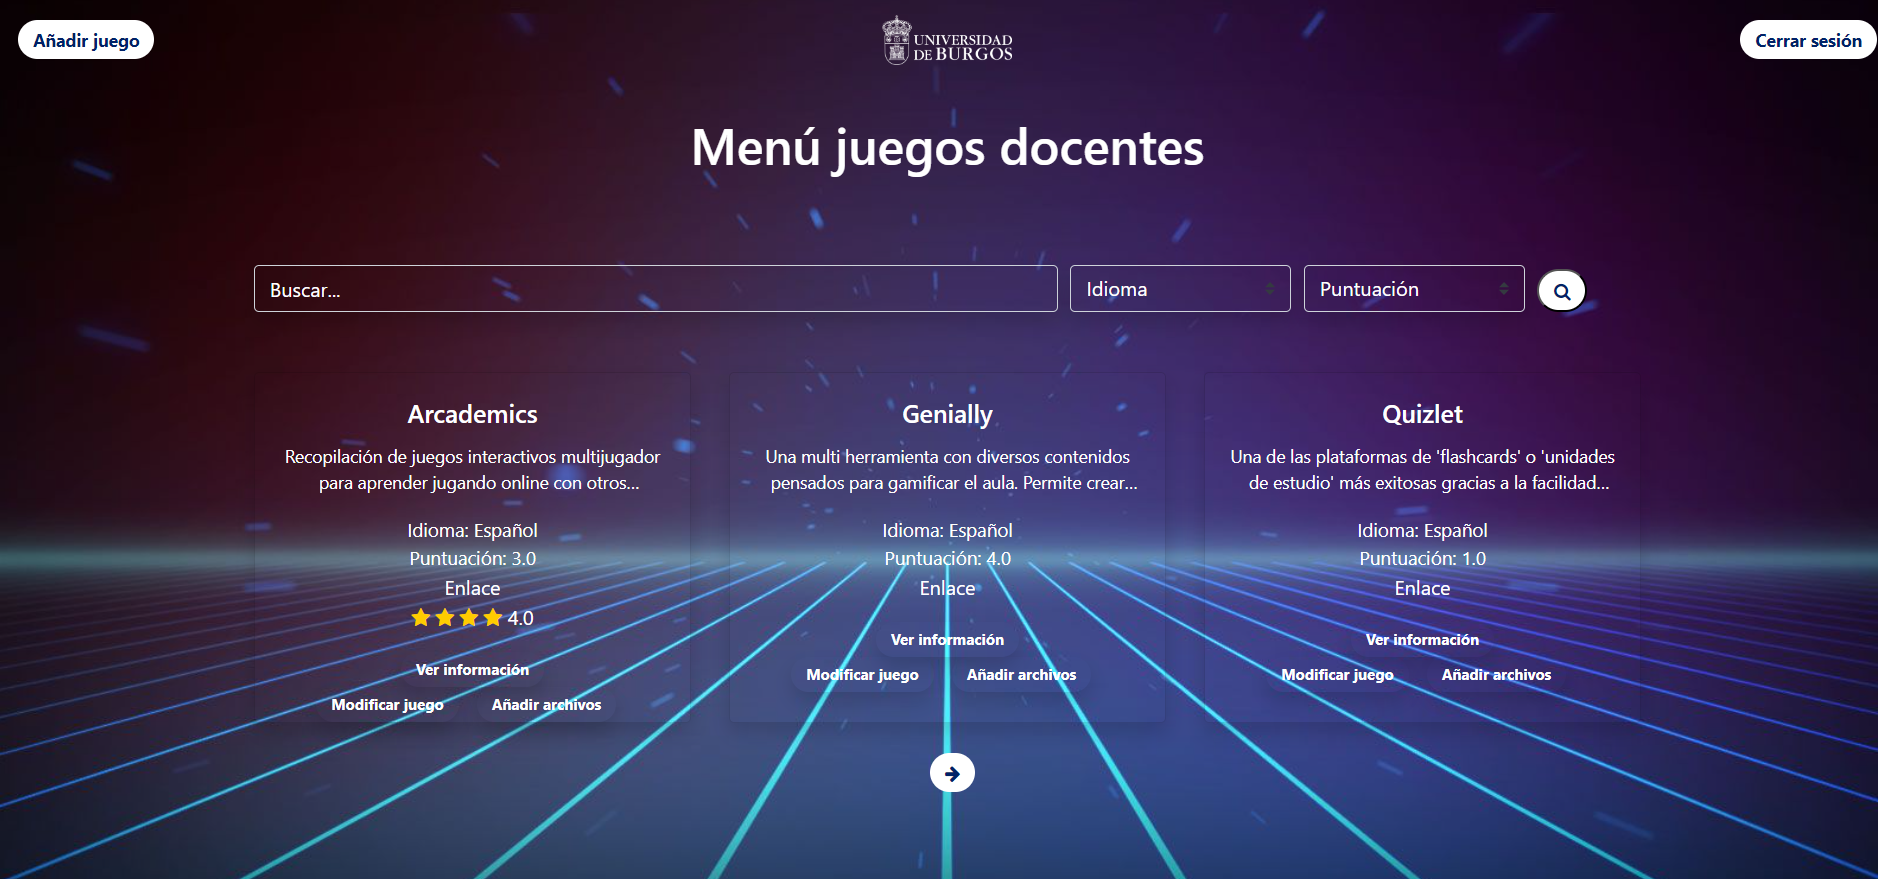
\includegraphics[width=0.8\textwidth]{menu-profesor}
\caption{Interfaz del menú de juegos de profesores.}
\label{fig:menu-profesor}
\end{figure}

Como se puede observar, el resultado final del menu\_juegos\_profesor.html presenta varias diferencias visuales en comparación con el prototipo inicial, al igual que con el menú de juegos de los usuarios. En el resultado final, la visualización de los juegos se presenta en tarjetas, lo cual facilita su visualización y ofrece una apariencia más atractiva. Además, se ha agregado la funcionalidad de realizar búsquedas utilizando tanto la barra de búsqueda como filtros, lo cual permite realizar búsquedas más específicas, al igual que en el menú de los usuarios. También se ha añadido un botón adicional para la subida de archivos a cada juego.

\subsection{Añadir nuevo juego}
La interfaz para añadir un juego nuevo está diseñada exclusivamente para los profesores. En el prototipo, se divide en diferentes secciones donde se debe ingresar información obligatoria sobre el juego que se desea incluir.

\begin{itemize}
    \item Categorización del juego: permite incluir el nombre del juego, su enlace si existe, su disciplina, su naturaleza, el idioma, el precio, las instrucciones del jugador y las notas para el instructor.
    \begin{figure}[htb]
    \centering
    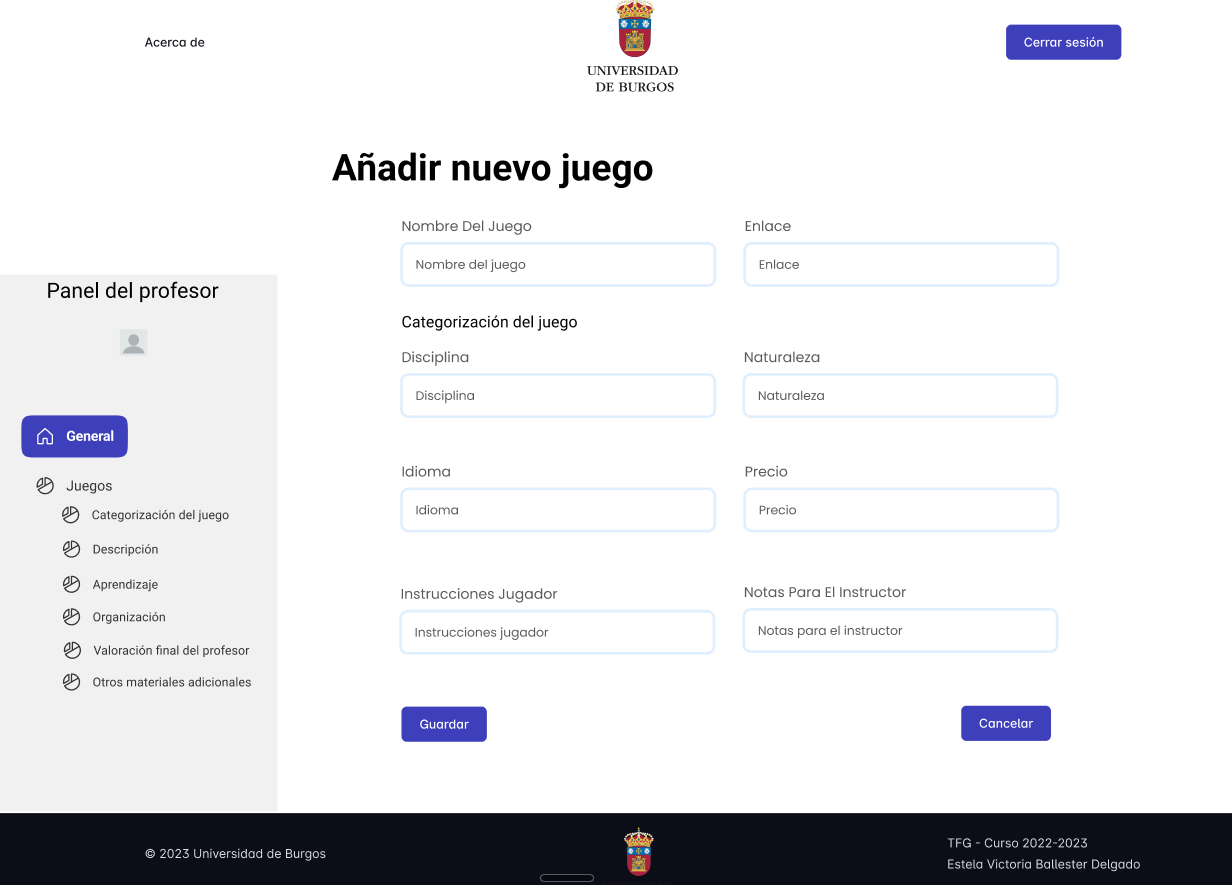
\includegraphics[width=0.7\textwidth]{añadir-juego1-prototipo}
    \caption{Prototipo de añadir la categorización del juego.}
    \label{fig:añadir-juego1-prototipo}
    \end{figure}
    \newpage
    \item Descripción: permite incluir el contexto del juego, los objetivos y el espacio de control.
    \begin{figure}[htb]
    \centering
    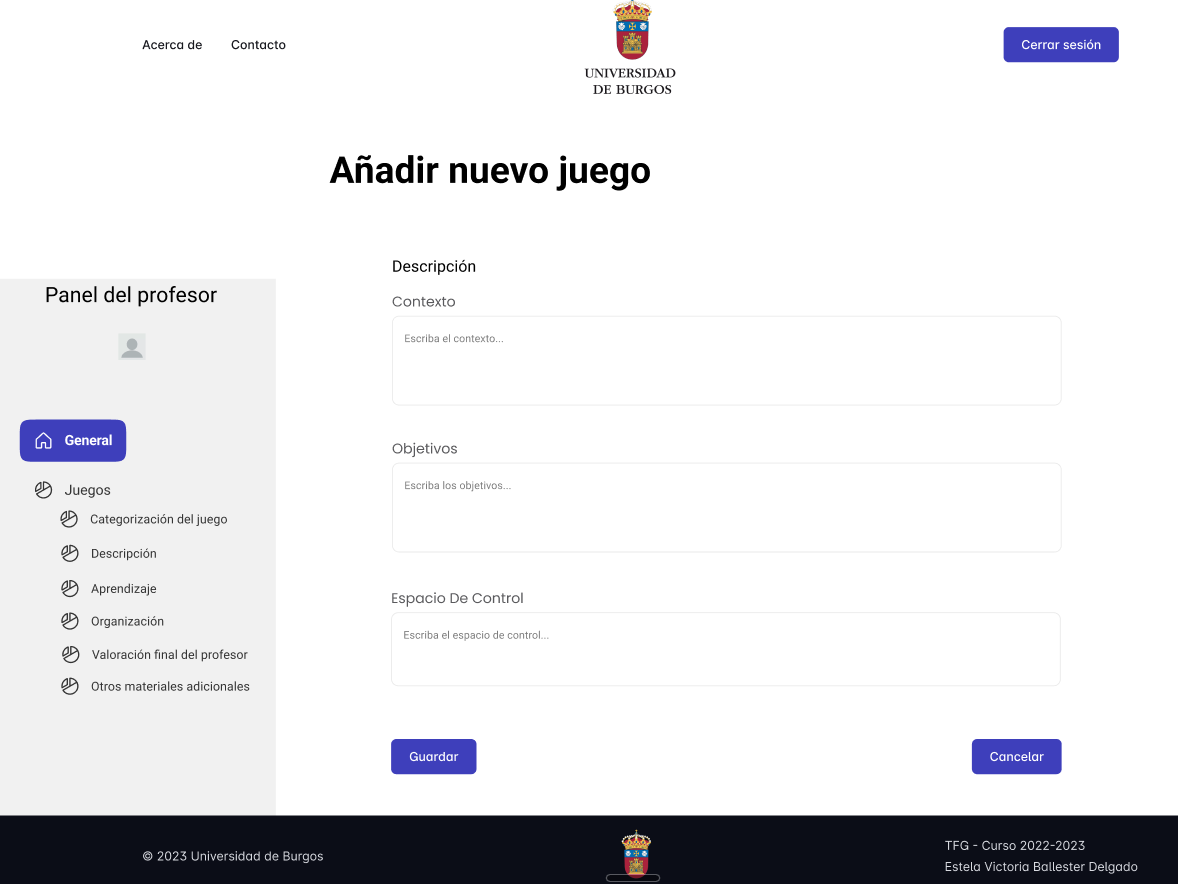
\includegraphics[width=0.7\textwidth]{añadir-juego2-prototipo}
    \caption{Prototipo de añadir la descripción del juego.}
    \label{fig:añadir-juego2-prototipo}
    \end{figure}
 
    \item Aprendizaje: permite incluir los objetivos principales y secundarios.
    \begin{figure}[htb]
    \centering
    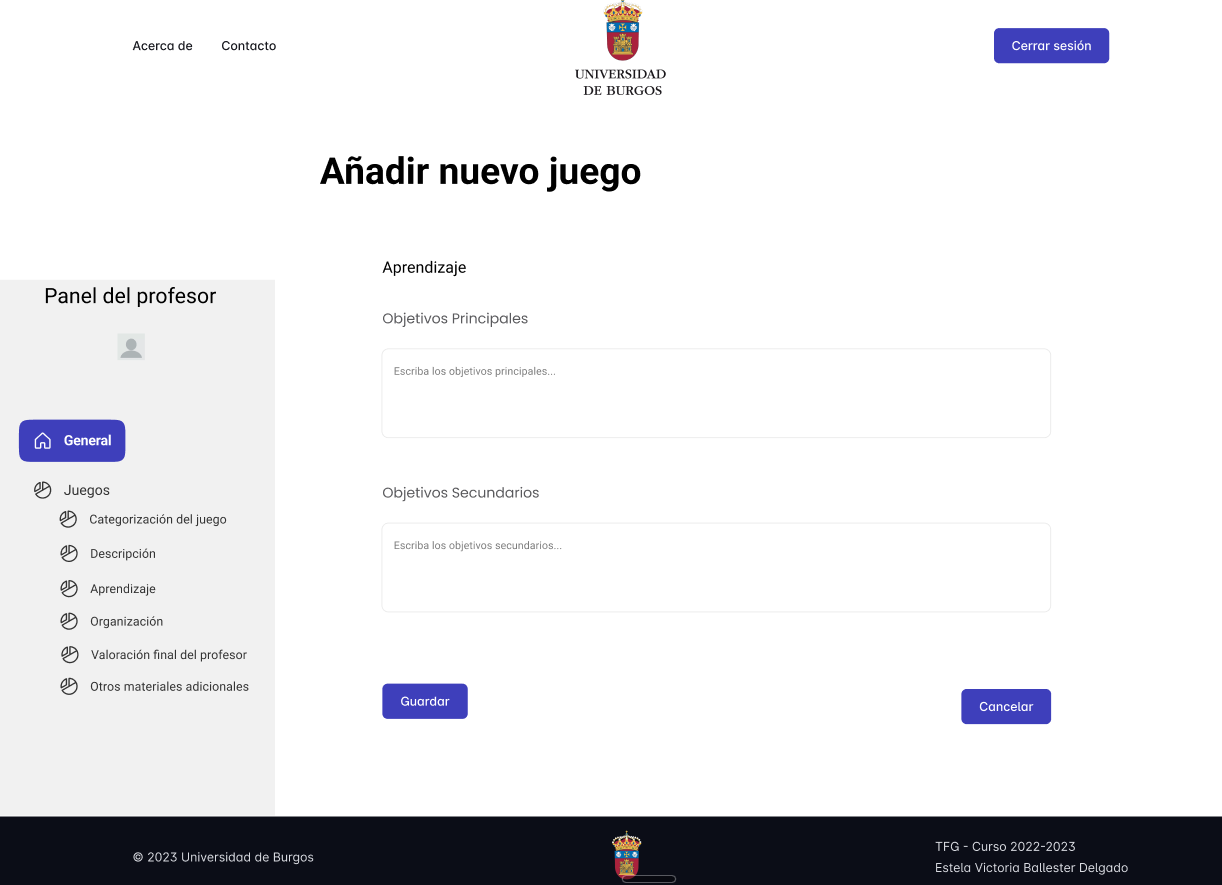
\includegraphics[width=0.7\textwidth]{añadir-juego3-prototipo}
    \caption{Prototipo de añadir el aprendizaje del juego.}
    \label{fig:añadir-juego3-prototipo}
    \end{figure}
    \newpage
    \item Organización: permite incluir la estructura propuesta para las sesiones y los aspectos adicionales a tener en cuenta.
    \begin{figure}[htb]
    \centering
    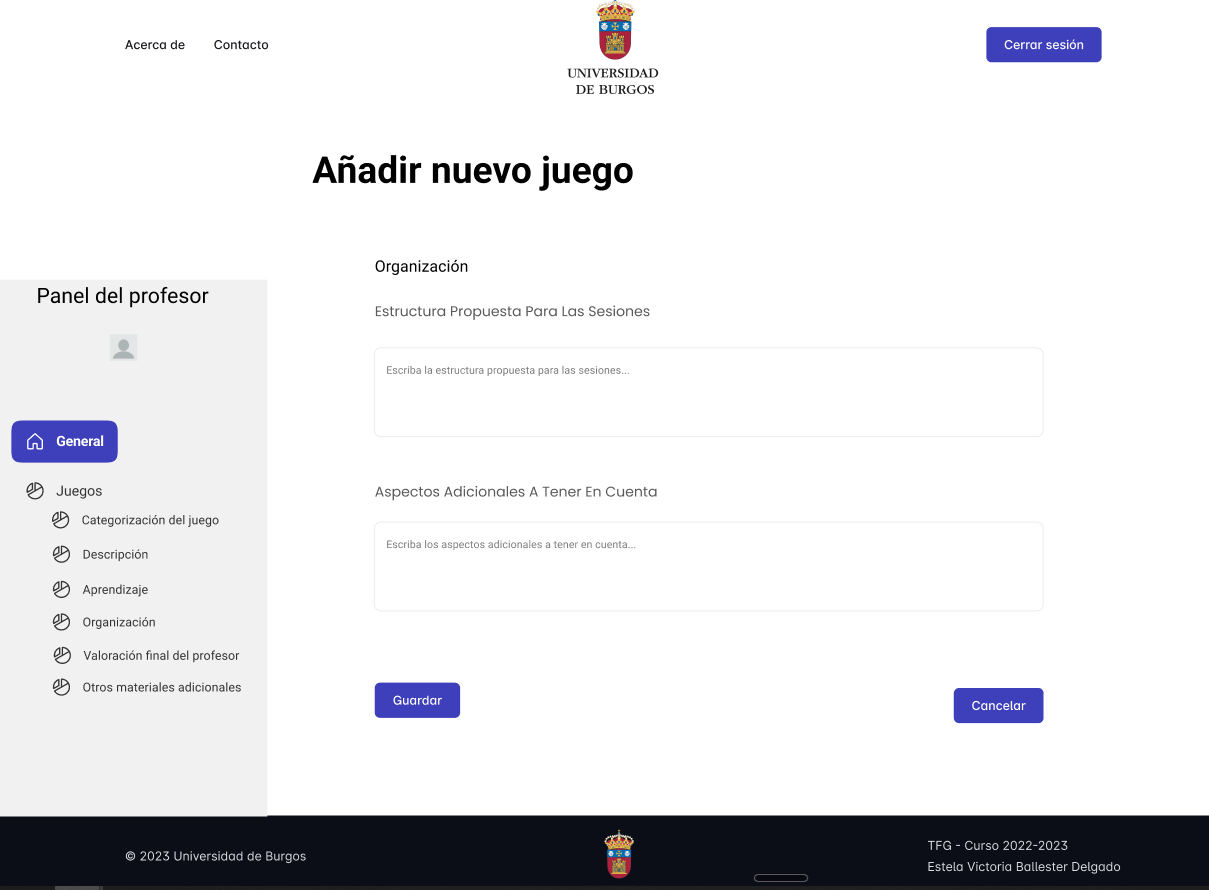
\includegraphics[width=0.6\textwidth]{añadir-juego4-prototipo}
    \caption{Prototipo de añadir la organización del juego.}
    \label{fig:añadir-juego4-prototipo}
    \end{figure}

    \item Valorización final del profesor: permite incluir la valoración del entretenimiento, el aprendizaje, la complejidad para el alumno y la complejidad para nuevos instructores.
    \begin{figure}[htb]
    \centering
    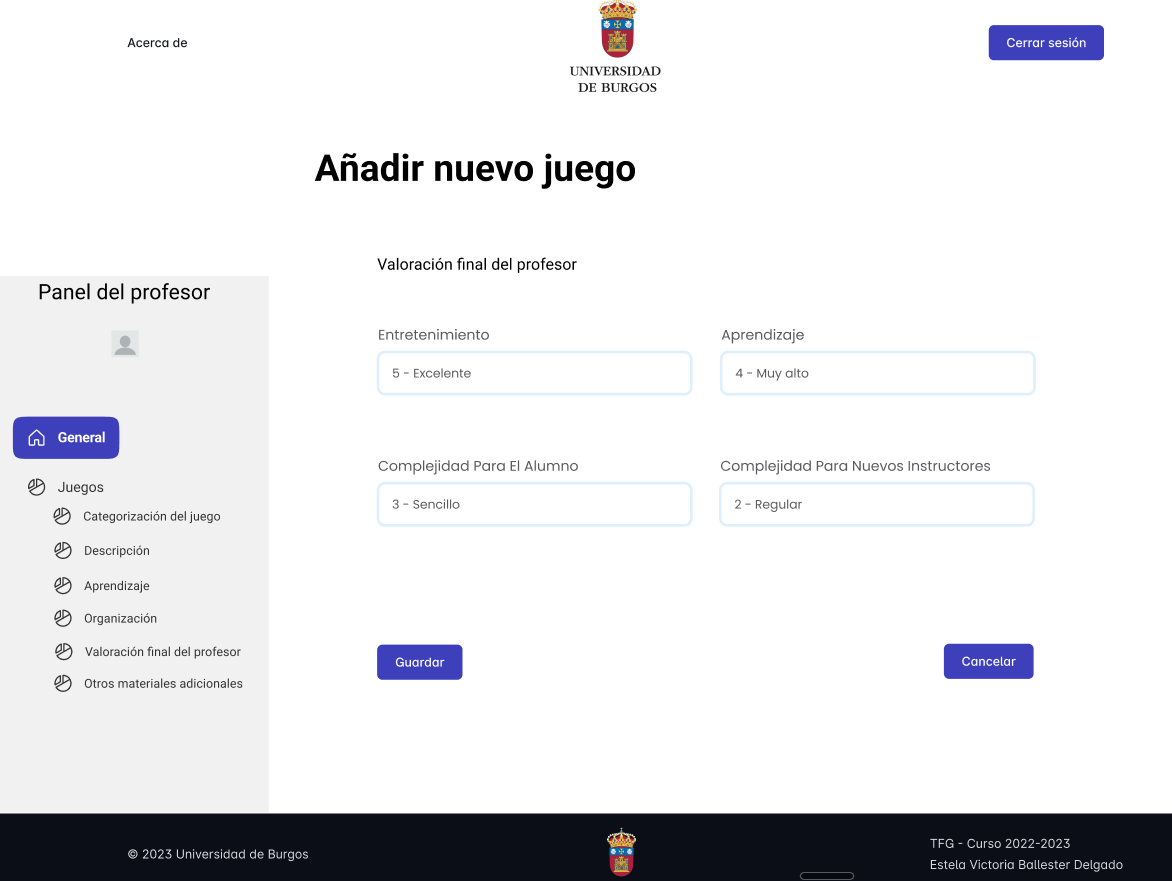
\includegraphics[width=0.7\textwidth]{añadir-juego5-prototipo}
    \caption{Prototipo de añadir la valorización final del profesor del juego.}
    \label{fig:añadir-juego5-prototipo}
    \end{figure}
\end{itemize}
\newpage

Finalmente, el resultado del template añadir\_juego.html quedó de la siguiente manera:

\begin{figure}[htb]
    \centering
    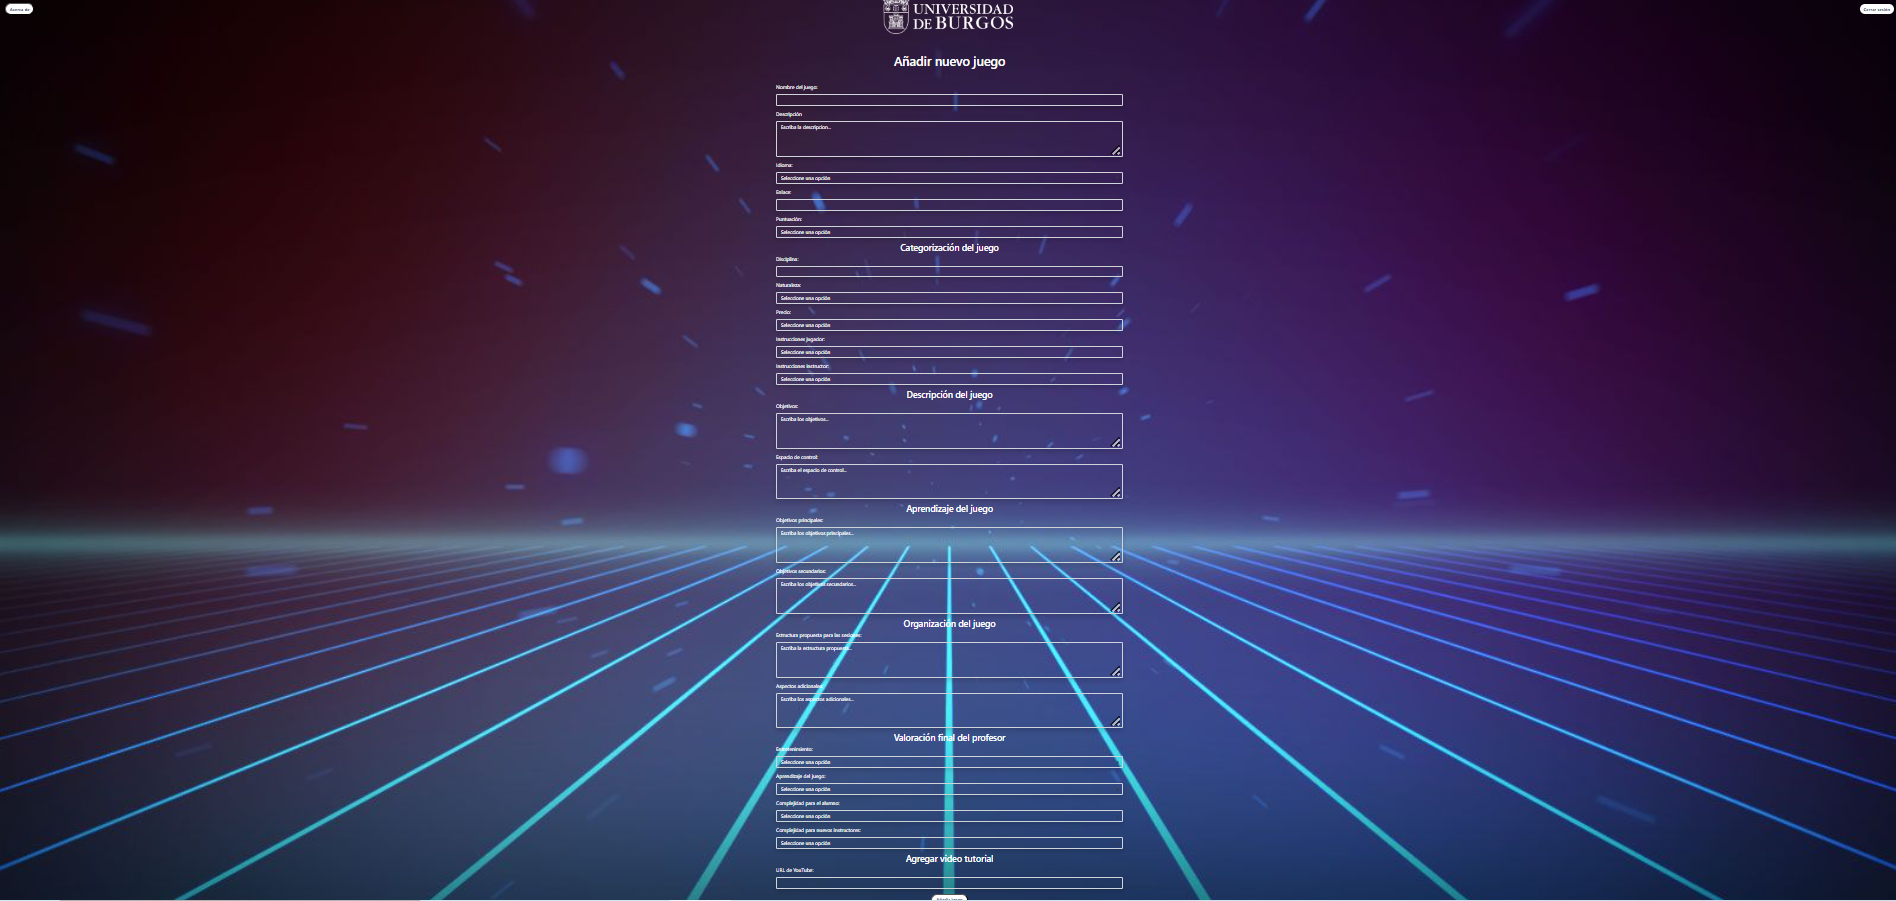
\includegraphics[width=0.8\textwidth]{añadir-juego}
    \caption{Interfaz de añadir juego.}
    \label{fig:añadir-juego}
    \end{figure}

Como se puede observar, el resultado final del template añadir\_juego.html presenta varias diferencias visuales en comparación con el prototipo inicial. En el prototipo, el proceso de añadir un nuevo juego se dividía en diferentes páginas, mientras que en el resultado final se ha unificado todo en una sola página. Además, se ha implementado la opción de añadir un enlace para un vídeo tutorial.

\subsection{Menú de juegos del administrador}
La interfaz del menú de juegos del administrador proporciona diversas funcionalidades. Permite realizar búsquedas personalizadas de los juegos, visualizar información detallada de cada juego, así como acceder al menú de administración.
\newpage

\begin{figure}[htb]
\centering
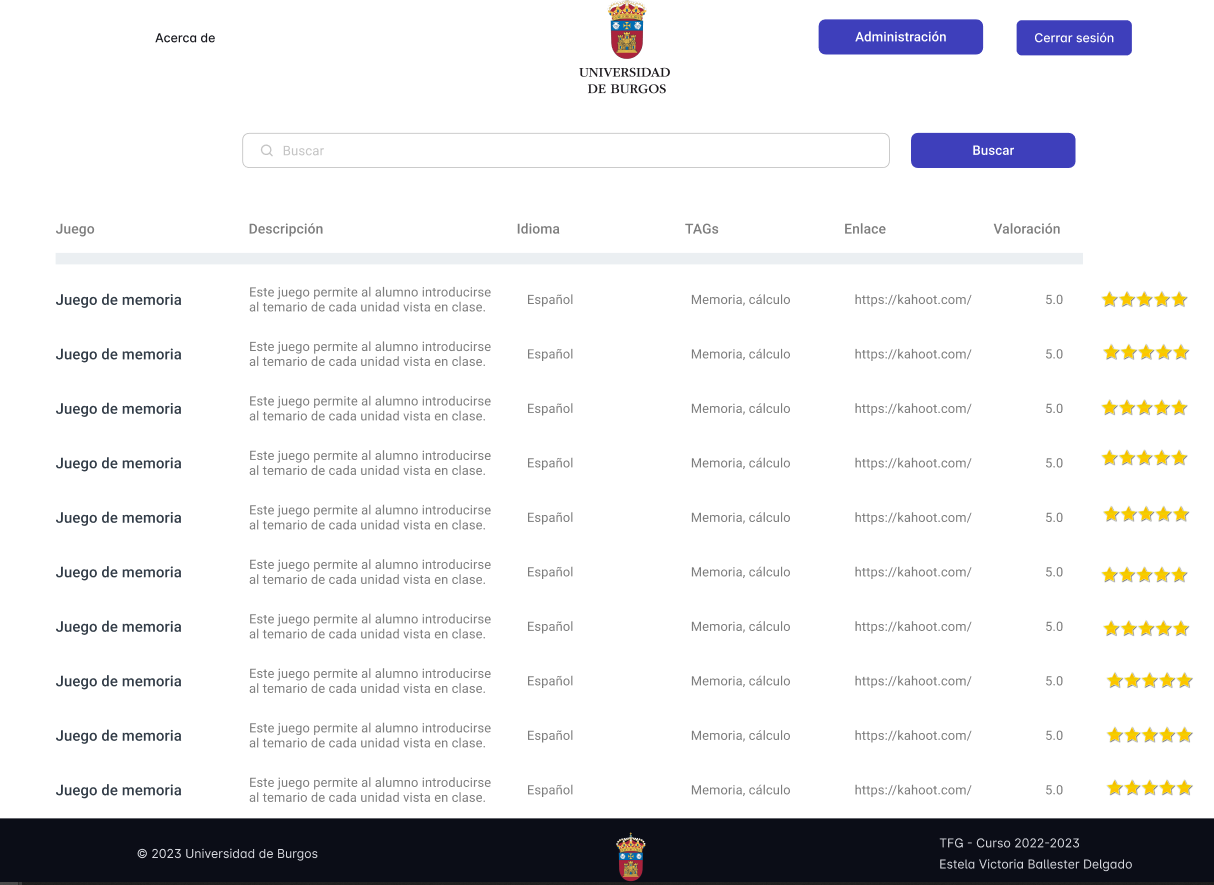
\includegraphics[width=0.7\textwidth]{menu-administrador-prototipo}
\caption{Prototipo del menú de juegos del administrador.}
\label{fig:menu-administrador-prototipo}
\end{figure}

Finalmente, el resultado del template menu\_juegos\_administrador.html quedó de la siguiente manera:

\begin{figure}[htb]
\centering
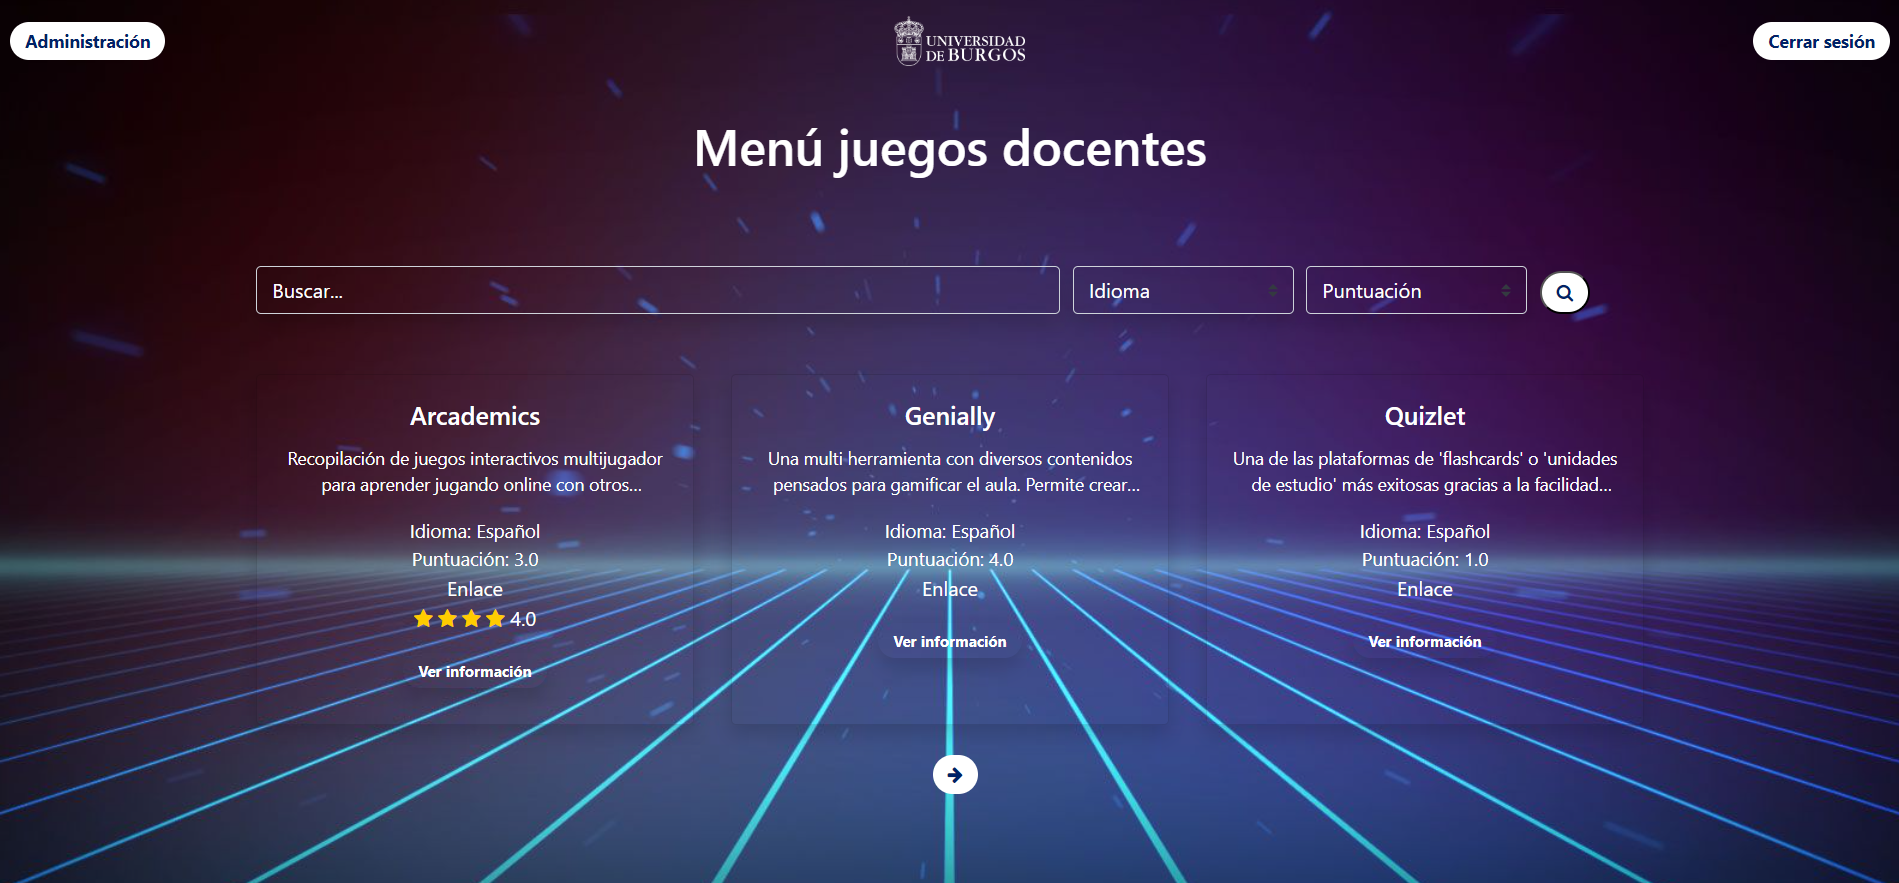
\includegraphics[width=0.8\textwidth]{menu-administrador}
\caption{Interfaz del menú de juegos del administrador.}
\label{fig:menu-administrador}
\end{figure}

Como se puede observar, el resultado final del template menu\_juegos\_administrador.html presenta varias diferencias visuales en comparación con el prototipo inicial, especialmente en lo que respecta a la visualización de los juegos. En el resultado final, se ha implementado la aplicación de filtros, al igual que en los otros menús, lo cual permite una búsqueda más precisa y específica de los juegos disponibles.

\subsection{Administración}
La interfaz de administración permite acceder a las funciones de gestión de juegos, usuarios y solicitudes.

\begin{figure}[htb]
\centering
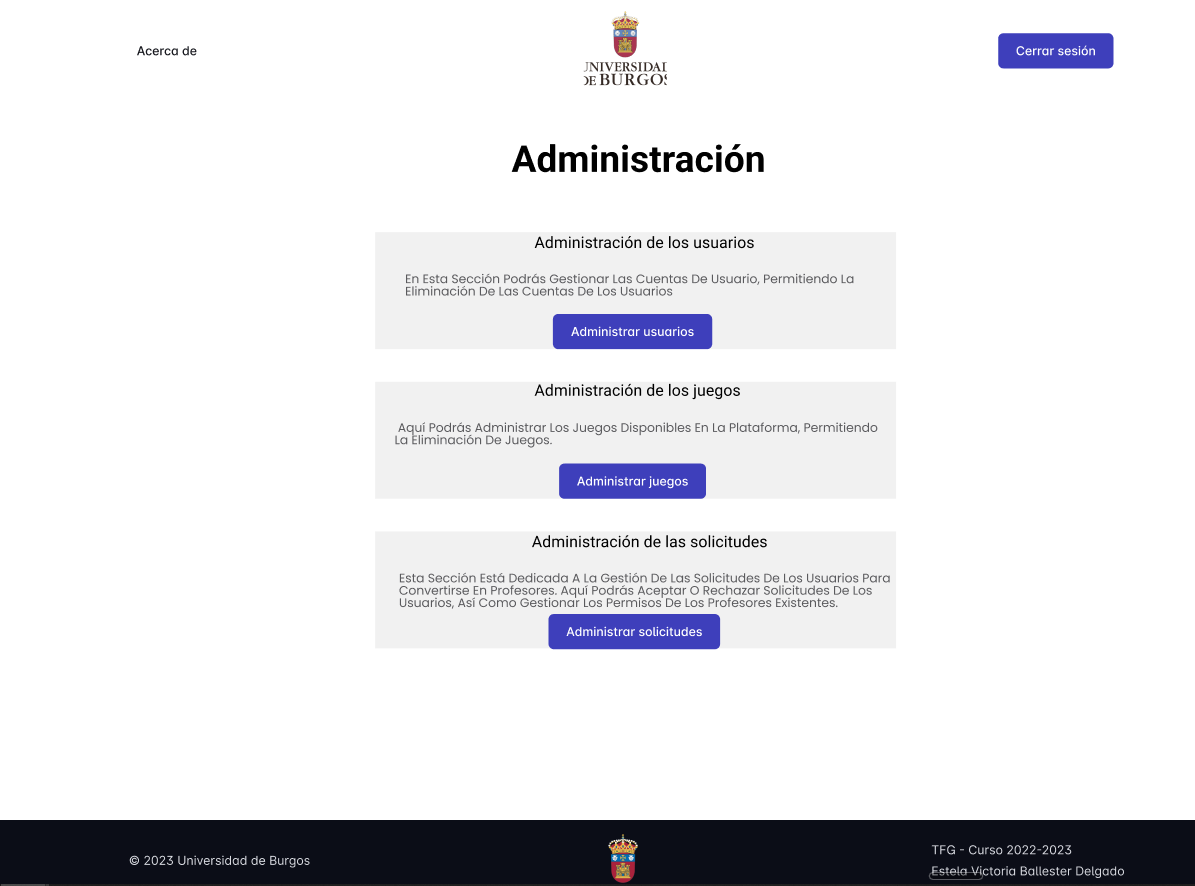
\includegraphics[width=0.7\textwidth]{administracion-prototipo}
\caption{Prototipo de la administración.}
\label{fig:administracion-prototipo}
\end{figure}

Finalmente, el resultado del template administracion.html quedó de la siguiente manera:

\begin{figure}[htb]
\centering
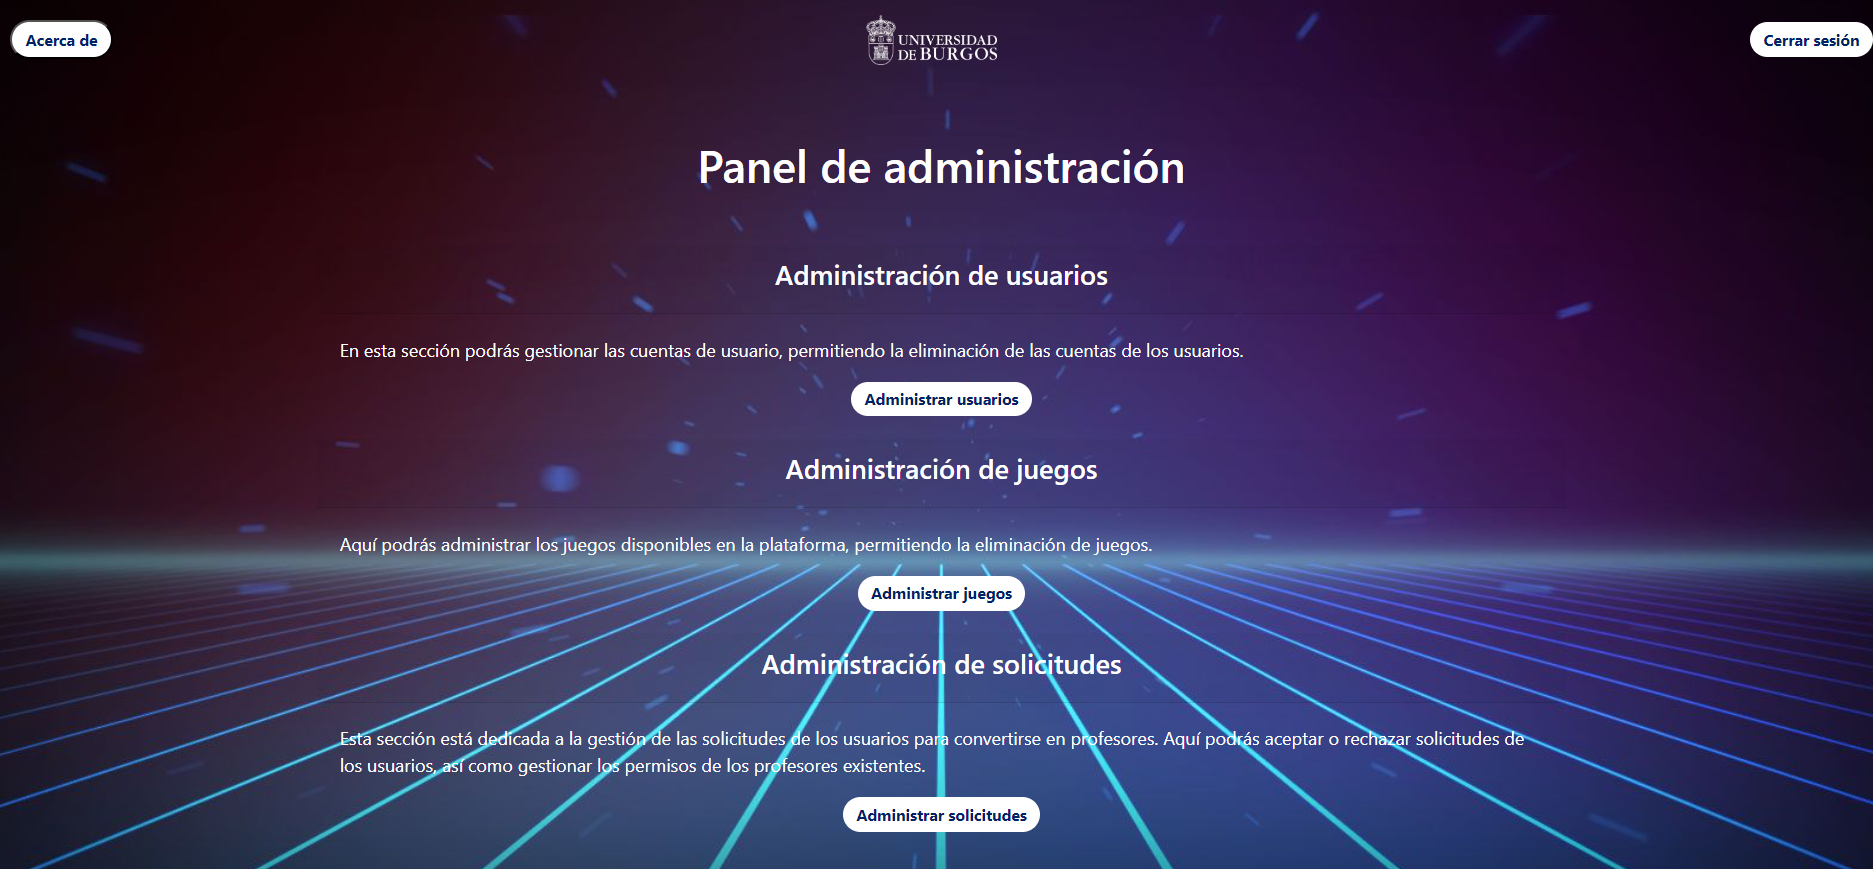
\includegraphics[width=0.8\textwidth]{administracion}
\caption{Interfaz de la administración.}
\label{fig:administracion}
\end{figure}

Como se puede observar, el resultado final del template administracion.html es prácticamente idéntico al prototipo inicial. 

\subsection{Administrar juegos}
La interfaz de los juegos solo es accesible por los administradores. Esta les permite visualizar información general de los juegos y borrarlos en el caso de que sea necesario.

\begin{figure}[htb]
\centering
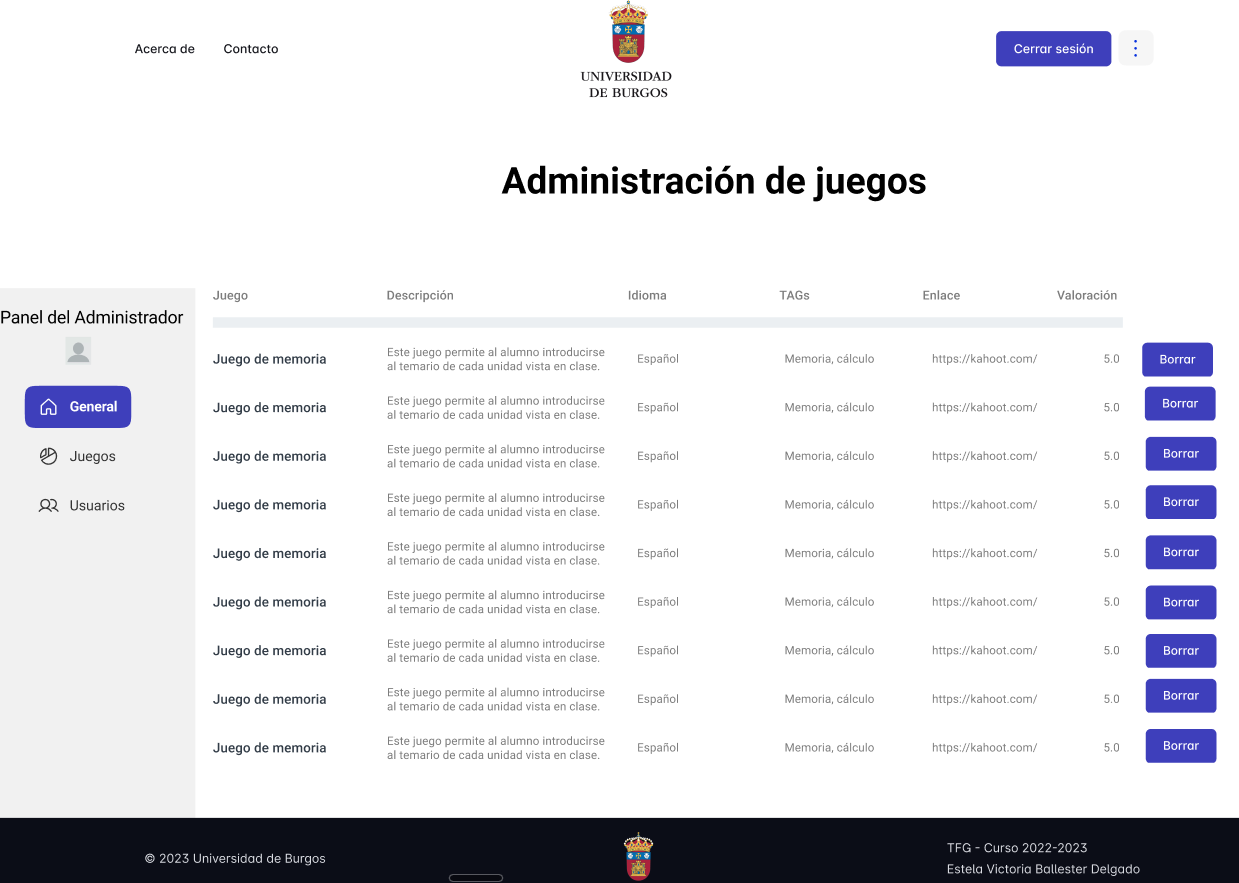
\includegraphics[width=0.7\textwidth]{admin-juegos-prototipo}
\caption{Prototipo de la administración de juegos.}
\label{fig:admin-juegos-prototipo}
\end{figure}

Finalmente, el resultado del template administrar\_juegos.html quedó de la siguiente manera:

\begin{figure}[htb]
\centering
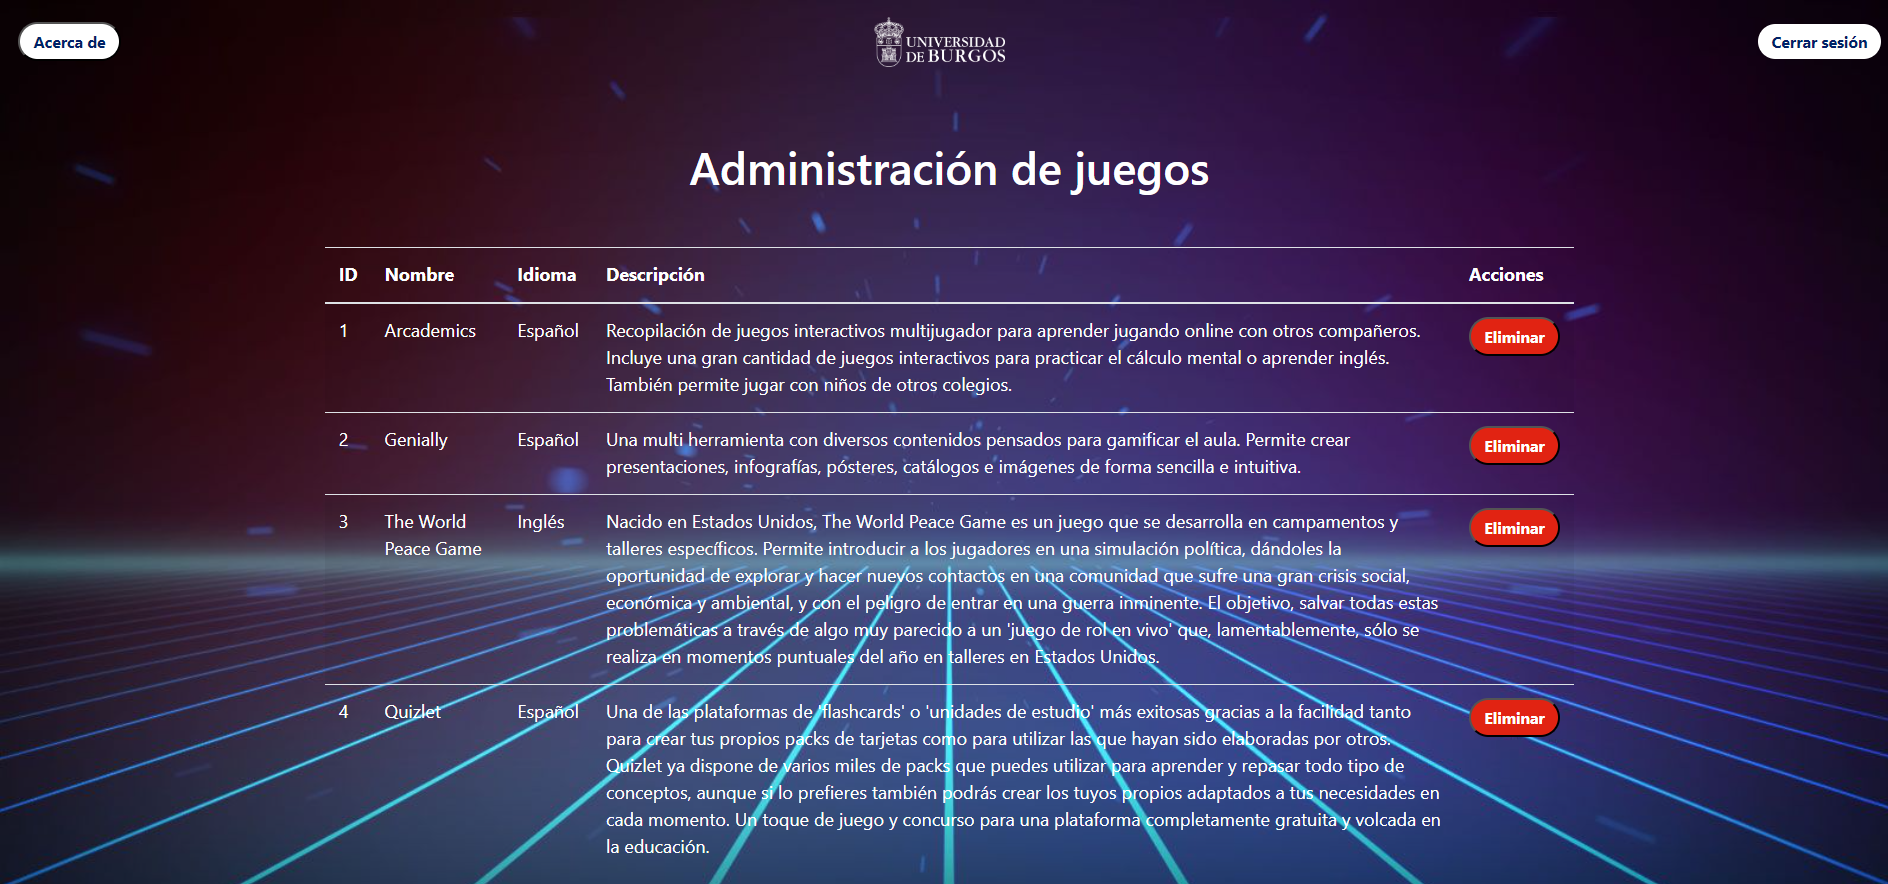
\includegraphics[width=0.8\textwidth]{administracion-juegos}
\caption{Interfaz de la administración de juegos.}
\label{fig:administracion-juegos}
\end{figure}

Como se puede observar, el resultado final del template administrar\_juegos.html es prácticamente idéntico al prototipo inicial. 

\subsection{Administrar usuarios}
La interfaz de gestión de los usuarios solo es accesible por los administradores. Esta les permite visualizar información general de los usuarios y borrarlos en el caso de que sea necesario.
\begin{figure}[htb]
\centering
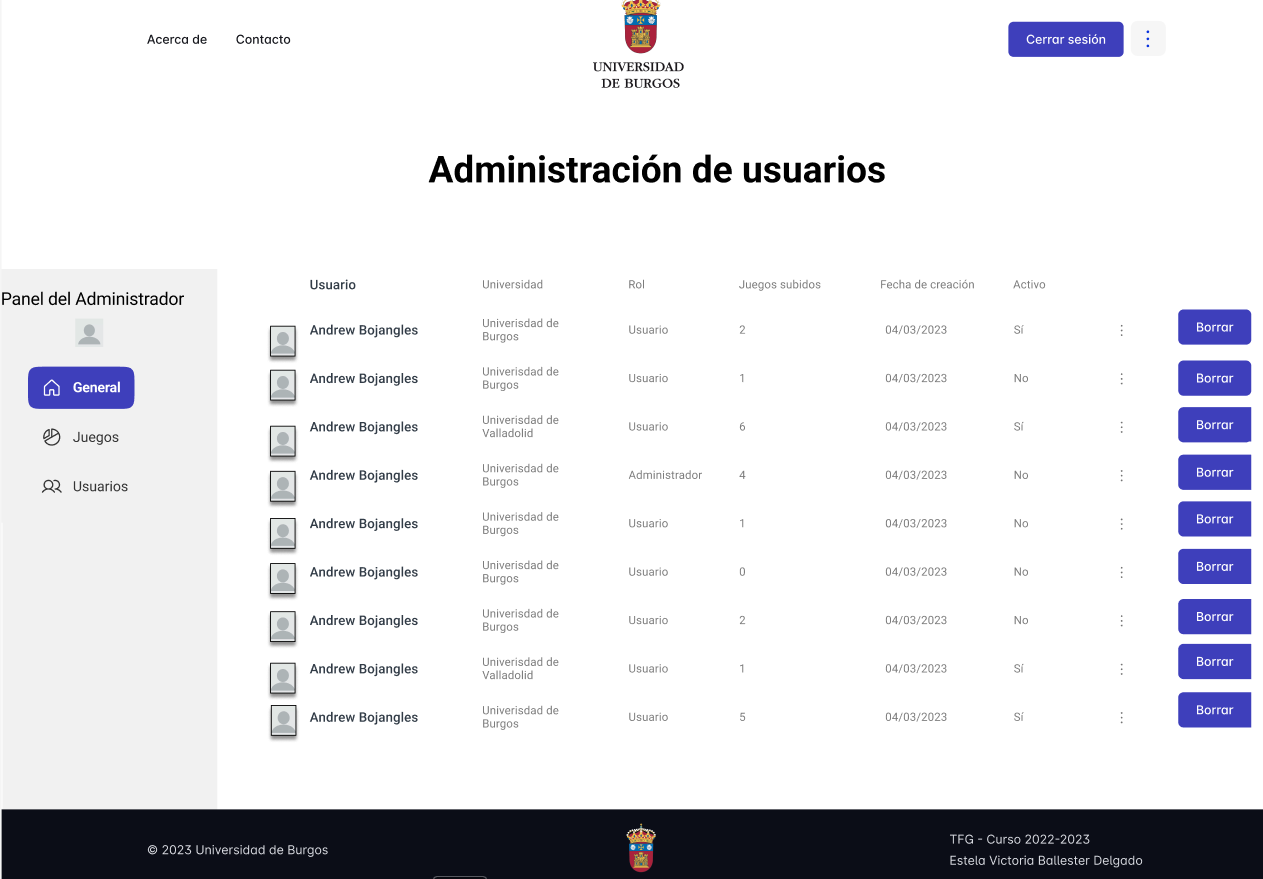
\includegraphics[width=0.7\textwidth]{admin-ususarios-prototipo}
\caption{Prototipo de la administración de los usuarios}
\label{fig:admin-ususarios-prototipo}
\end{figure}

Finalmente, el resultado del template administrar\_usuarios.html quedó de la siguiente manera:

\begin{figure}[htb]
\centering
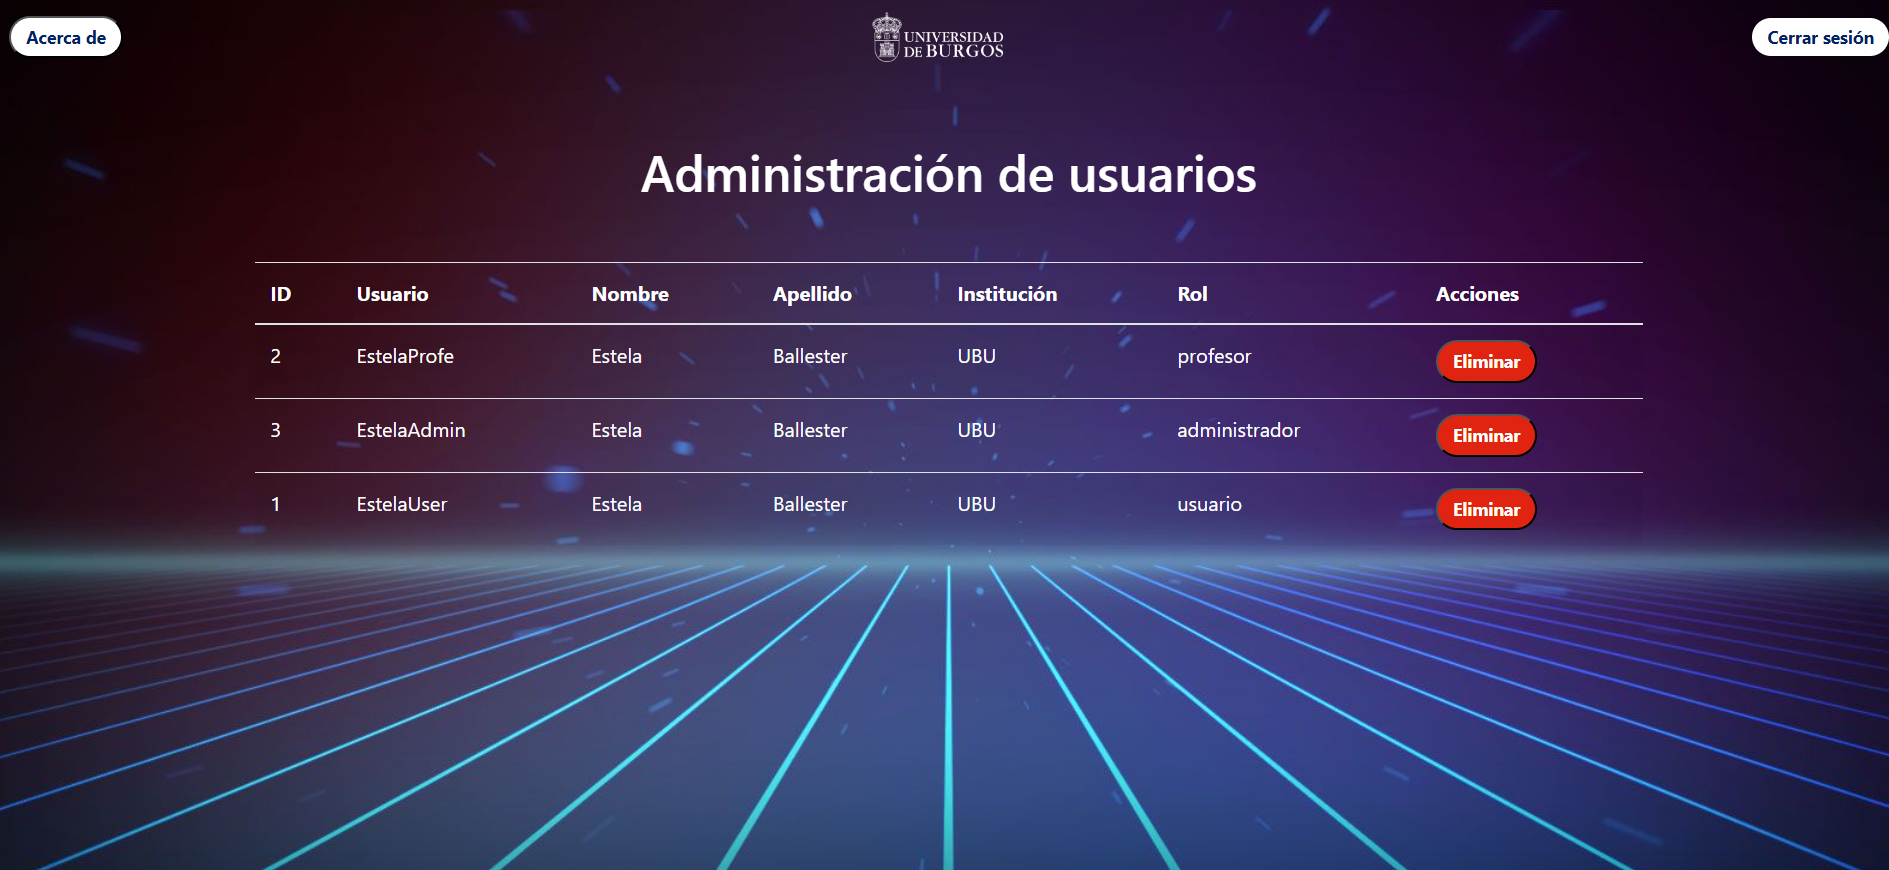
\includegraphics[width=0.8\textwidth]{administracion-usuarios}
\caption{Interfaz de la administración de usuarios.}
\label{fig:administracion-usuarios}
\end{figure}

Como se puede observar, el resultado final del template administrar\_usuarios.html es prácticamente idéntico al prototipo inicial. 

\subsection{Administrar solicitudes}
La interfaz de gestión de las solicitudes solo es accesible por los administradores. Esta les permite visualizar información general de las solicitudes y aprobarlas o rechazarlas.

\begin{figure}[htb]
\centering
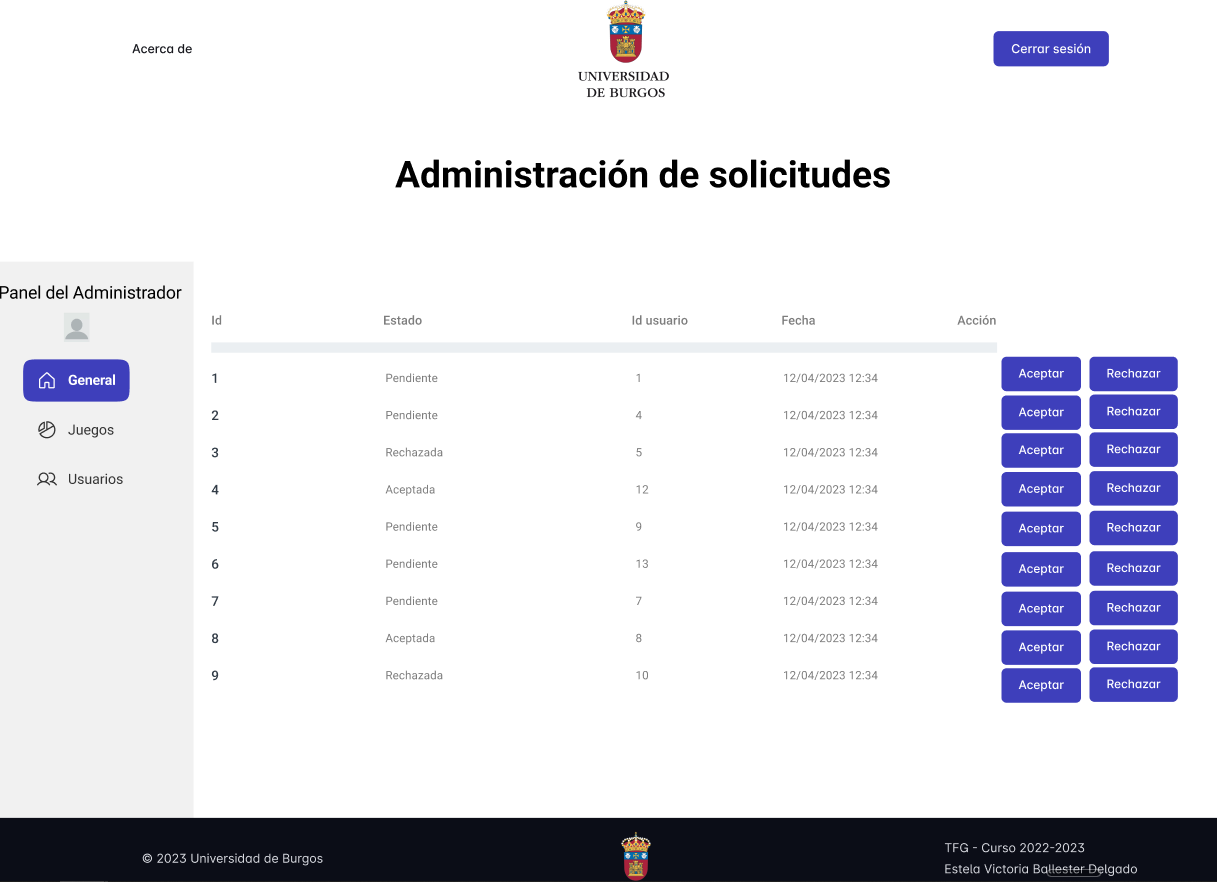
\includegraphics[width=0.7\textwidth]{admin-solicitudes-prototipo}
\caption{Prototipo de la administración de las solicitudes}
\label{fig:admin-solicitudes-prototipo}
\end{figure}
Finalmente, el resultado del template administrar\_solicitudes.html quedó de la siguiente manera:

\begin{figure}[htb]
\centering
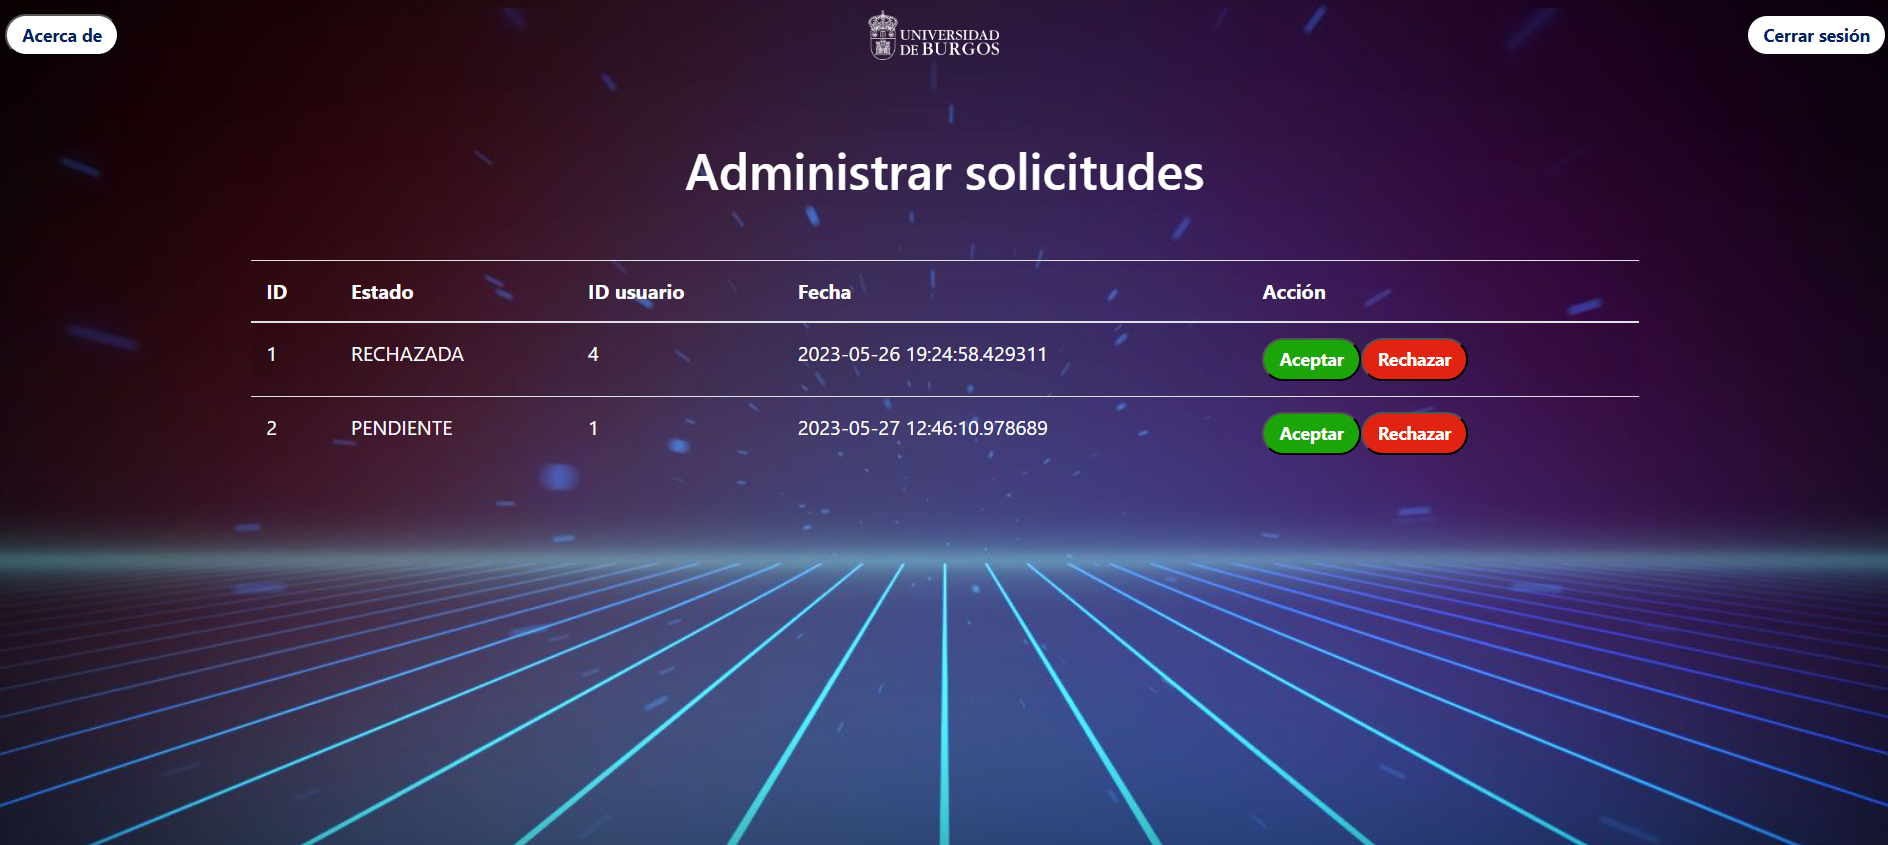
\includegraphics[width=0.8\textwidth]{administracion-solicitudes}
\caption{Interfaz de la administración de solicitudes.}
\label{fig:administracion-solicitudes}
\end{figure}

Como se puede observar, el resultado final del template administrar\_solicitudes.html es prácticamente idéntico al prototipo inicial. 

\subsection{Acerca de}
La interfaz de acerca está disponible para todos los usuarios, independientemente de su rol. En esta página se muestra información general sobre la aplicación.

\begin{figure}[htb]
\centering
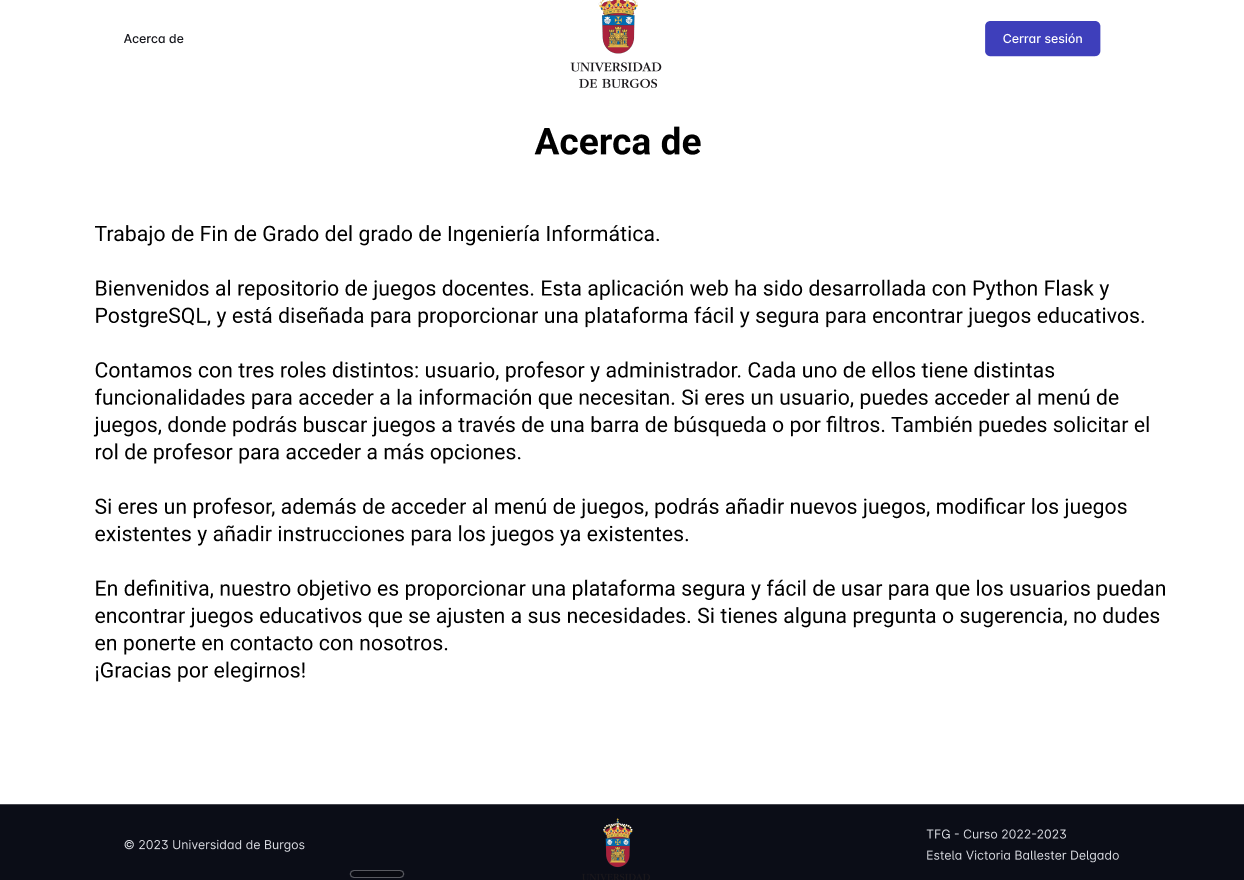
\includegraphics[width=0.7\textwidth]{acerca-prototipo}
\caption{Prototipo de acerca de.}
\label{fig:acerca-prototipo}
\end{figure}
Finalmente, el resultado del template acerca\_de.html quedó de la siguiente manera:

\begin{figure}[htb]
\centering
\includegraphics[width=0.8\textwidth]{acerca}
\caption{Interfaz de acerca de.}
\label{fig:acerca}
\end{figure}

Como se puede observar, el resultado final del template acerca\_de.html es prácticamente idéntico al prototipo inicial. 

\subsection{Modificar juego}
La interfaz de modificar un juego permite al profesor modificar la información de cada juego.
\begin{figure}[htb]
\centering
\includegraphics[width=0.7\textwidth]{modificar-juego-prototipo}
\caption{Prototipo de la modificación de juegos.}
\label{fig:modificar-juego-prototipo}
\end{figure}

Finalmente, el resultado del template modificar\_juego.html quedó de la siguiente manera:
\newpage
\begin{figure}[htb]
\centering
\includegraphics[width=0.8\textwidth]{modificar-juego}
\caption{Interfaz de la modificación de juegos.}
\label{fig:modificar-juego}
\end{figure}

Como se puede observar, el resultado final del template modificar\_juego.html es prácticamente idéntico al prototipo inicial. 

\subsection{Visualizar juego}
La interfaz de visualizar un juego permite los usuarios ver la información específica de cada juego.
\newpage
\begin{figure}[htb]
\centering
\includegraphics[width=0.7\textwidth]{visualizar-juego-prototipo}
\caption{Prototipo de la visualización de juegos.}
\label{fig:visualizar-juego-prototipo}
\end{figure}
Finalmente, el resultado del template visualizar\_juego.html quedó de la siguiente manera:
\newpage
\begin{figure}[htb]
\centering
\includegraphics[width=0.8\textwidth]{visualizar-juego}
\caption{Interfaz de la visualización de juegos.}
\label{fig:visualizar-juego}
\end{figure}

Como se puede observar, el resultado final del template visualizar\_juego.html es prácticamente idéntico al prototipo inicial. 

Al tratarse de una aplicación responsive, está disponible para ser utilizada en otros dispositivos. A continuación, se muestra cómo se visualizan las interfaces en un dispositivo móvil.
\begin{figure}[htb]
\centering
\includegraphics[width=0.8\textwidth]{interfaces-movil}
\caption{Interfaces desde dispositivo móvil.}
\label{fig:interfaces-movil}
\end{figure}
\apendice{Documentación técnica de programación}

\section{Introducción}
En esta sección, se proporcionará una explicación y una muestra de la estructura organizativa del proyecto, así como el manual del programador y los pasos necesarios para ejecutar el proyecto.

\section{Estructura de directorios}
La estructura del proyecto se divide en diferentes directorios:

\begin{itemize}
    \item \textbf{/Documentación:} carpeta que contiene los documentos de la memoria y anexos del proyecto.
    \item \textbf{/env:} contiene los directorios con ejecutables que determinan que se trata de un entorno virtual.
    \item \textbf{/src:} carpeta que contiene todos los archivos Python relacionados con el funcionamiento del backend de la aplicación.
    \item \textbf{/static:} carpeta que contiene los archivos estáticos relacionados con el frontend, incluyendo el archivo de los estilos aplicados y la carpeta con las imágenes usadas en la aplicación
    \item \textbf{/templates:} carpeta que contiene todos los archivos HTML que forman la parte visual de la aplicación.
    \item \textbf{/translations:} carpeta que contiene los archivos JSON empleados para almacenar las traducciones de los HTMLs, y el archivo que se encarga de cargar las traducciones desde los archivos JSON correspondientes.
    \item \textbf{/uploads:} carpeta oculta que contiene los archivos que subieron los usuarios durante el uso de la aplicación.
    \item \textbf{/videos:} carpeta que contiene los vídeos que muestran el uso de la aplicación.
    \item \textbf{.env:} archivo oculto que contiene las contraseñas necesarias para la conexión a la base de datos.
    \item \textbf{.gitignore:} archivo que contiene el nombre de los archivos que se encuentran ocultos en GitHub.
    \item \textbf{app.py:} archivo principal de Python que contiene todos los métodos GET y POST de la aplicación. 
    \item \textbf{errores.log:} archivo oculto que contiene el registro de los errores que se generan durante la ejecución de la aplicación.
    \item \textbf{LICENSE:} licencia de la aplicación.
    \item \textbf{Procfile:} archivo en el que se determina el archivo principal de la aplicación para el despliegue en Heroku. 
    \item \textbf{README.md:} archivo que contiene la descripción del proyecto junto con los pasos necesarios para su uso.
    \item \textbf{requirements.txt:} archivo que contiene las herramientas junto con sus versiones, para ejecutar el despliegue en Heroku.
   
\end{itemize}

\section{Manual del programador}
En este manual se van a indicar los diferentes procedimientos que debe seguir el programador para la correcta preparación y ejecución del proyecto.

El proyecto ha sido desarrollado inicialmente de forma local en el equipo y posteriormente se ha desplegado en Heroku, por lo que se encuentra disponible en este enlace: \url {https://teachmeplay.herokuapp.com/}. Para la realización de pruebas para cargar correctamente los archivos de los juegos se dispondrá de una máquina virtual como simulación del equipo local.

\subsection{Visual Studio Code}
Visual Studio Code se emplea para el desarrollo de la aplicación web y la creación de todos los archivos y métodos necesarios para el correcto uso y funcionamiento del proyecto.

Para descargar Visual Studio Code, se debe acceder a la página web oficial en \url{https://code.visualstudio.com/download}. Después, se debe seleccionar la versión adecuada para el sistema operativo, en este caso, la versión utilizada es la de Windows.

Una vez completada la descarga, se procede a instalar Visual Studio Code siguiendo los pasos correspondientes.

\subsection{Python}
Como lenguaje de programación se ha utilizado Python. Para descargar Python, se debe acceder a la página web oficial en \url{https://www.python.org/downloads/} y pulsar el botón de descargar la última versión disponible. En este caso, la versión descargada es Python 3.11.3.

Una vez completada la descarga, se procede a instalar Python siguiendo los pasos correspondientes.

\subsection{PostgreSQL}
Para la gestión de la base de datos se ha utilizado PostgreSQL. Para descargar PostgreSQL, se debe acceder a la página web oficial en \url{https://www.postgresql.org/download/} y seleccionar la versión adecuada para el sistema operativo. En este caso, la versión utilizada es la de Windows y la última versión disponible es la versión 15 de 64 bits.

Una vez completada la descarga, se procede a instalar PostgreSQL siguiendo los pasos correspondientes.

Cuando ya se tiene instalado se debe configurar para poder acceder a la base de datos de Heroku. 

Para ello, se debe crear un nuevo servidor.
\newpage
    \begin{figure}[htbp]
    \centering
    \includegraphics[width=0.7\textwidth]{server}
    \caption{Crear nuevo servidor.}
    \label{fig:server}
    \end{figure}

Este se configura con los datos que obtenemos del Add-on de Heroku. Se debe rellenar el nombre del servidor en la pestaña ``General``.
    \begin{figure}[htbp]
    \centering
    \includegraphics[width=0.3\textwidth]{server1}
    \caption{Crear nuevo servidor: general.}
    \label{fig:server1}
    \end{figure}
    
Se debe rellenar el nombre del host, el puerto, el nombre de usuario, base de datos y la contraseña en la pestaña ``Connection``.
\newpage
    \begin{figure}[htbp]
    \centering
    \includegraphics[width=0.3\textwidth]{server2}
    \caption{Crear nuevo servidor: connection.}
    \label{fig:server2}
    \end{figure}
    
Y, por último, se debe rellenado el campo de DB restriction en la pestaña ``Advanced``.
    \begin{figure}[htbp]
    \centering
    \includegraphics[width=0.3\textwidth]{server3}
    \caption{Crear nuevo servidor: advanced.}
    \label{fig:server3}
    \end{figure}

\subsection{Virtual Box}
El proyecto está disponible en una máquina virtual para poder realizar pruebas en local. De esta forma se permite cargar los distintos archivos de los juegos que se admiten en la aplicación, que debido a las limitaciones de Heroku, no se permite comprobar su funcionamiento en la aplicación desplegada.

Para ello, se empleará VirtualBox, que ha sido utilizado en diversas asignaturas del grado. Esta herramienta ofrece una interfaz de usuario sencilla y un buen rendimiento.

Para su instalación se debe acceder a la página oficial disponible en \url{https://www.virtualbox.org/}, en la sección de descargas,  seleccionar la versión y paquete deseado siguiendo los pasos que se indican.

Como sistema operativo se ha usado Windows 10 Pro obtenido mediante la compra de una licencia OEM. La descarga de la ISO se realiza a través de la página oficial \url{https://www.microsoft.com/es-es/software-download/windows10} seleccionando la última versión disponible.

Una vez se tiene todo instalado se debe crear una máquina dentro del VirtualBox a través del botón de ``Nueva``, asignado el nombre de la máquina virtual y el sistema operativo que se va a instalar.
    \begin{figure}[htbp]
    \centering
    \includegraphics[width=0.6\textwidth]{vb}
    \caption{Creación de máquina virtual.}
    \label{fig:vb}
    \end{figure}
    
Posteriormente se deben seguir los pasos seleccionando la RAM que se desea y la creación de un disco duro VDI. Para instalar el sistema operativo de Windows 10 en la máquina creada, se debe hacer a través de la configuración añadiendo una unidad óptica y seleccionando el archivo ISO que se obtuvo anteriormente.

Por último, cuando se inicie la máquina virtual creada aparecerá la instalación de Windows, por lo que será necesario introducir la clave de la licencia comprada.

Cuando la máquina virtual ya está lista para su uso, se procede a la instalación de Python, Visual Studio Code y PostgreSQL, siguiendo los pasos descritos anteriormente. Después, se importan todos los archivos necesarios en la máquina y se configura la base de datos.

Finalmente, se exporta la máquina virtual mediante la opción de ``Exportar servicio virtualizado``.

\section{Compilación, instalación y ejecución del proyecto}
Para la ejecución del proyecto, se puede realizar de dos formas.
El proyecto puede ejecutarse en local desde la máquina virtual que se proporciona, o mediante el enlace de la página web en el que se encuentra desplegado en Heroku.

\subsection{Ejecución en local}
Para la ejecución en local se proporciona una máquina virtual de VirtualBox con sistema operativo Windows 10 y con todas la herramientas necesarias instaladas.

El objetivo de la máquina virtual es que se pueda ejecutar de forma rápida en local para probar todas las funcionalidades de la aplicación, ya que debido a las restricciones de Heroku no se permite ni cargar ni descargar los archivos de los juegos en la aplicación desplegada.

Para acceder a la sesión de la máquina virtual se debe introducir el PIN: ``0806``.
Una vez iniciada la sesión para ejecutar la aplicación se debe abrir Visual Studio Code e ingresar en el terminal los comandos:
\begin{itemize}
    \item env\textbackslash Scripts\textbackslash activate
    \item flask run
\end{itemize}

También, en el escritorio de la máquina se dispone de un archivo ``ejecutable.bat``, para que al acceder a éste, se ejecuten los comandos necesarios para activar tanto el entorno virtual como para ejecutar el proyecto.

El acceso a la aplicación web está disponible a través del siguiente enlace \url{http://127.0.0.1:5000/}

\subsection{Despliegue en Heroku}
Para desplegar la aplicación en Heroku es necesario obtener el paquete de desarrollo para estudiantes de GitHub para obtener beneficios por ser estudiante, lo cual permite obtener unos créditos para usar dentro de Heroku ya que se van a usar funcionalidades de pago.

Para desplegar el proyecto en Heroku, lo primero que se debe hacer es
registrarse en su página web en el siguiente enlace: \url{https://www.heroku.com/home}

Después de haberse registrado e iniciado sesión, para crear una aplicación se debe pulsar el botón New, donde habrá que establecer un nombre para la aplicación y elegir una región.
    \begin{figure}[htbp]
    \centering
    \includegraphics[width=0.7\textwidth]{new-app}
    \caption{Crear nueva aplicación en Heroku.}
    \label{fig:new-app}
    \end{figure}

Una vez creada la nueva aplicación, en la pestaña ``Deploy``, se muestran las opciones y los pasos a seguir para ejecutar el proyecto. Para ello, se debe elegir el método de despliegue en nuestro caso será con GitHub.
\newpage
    \begin{figure}[htbp]
    \centering
    \includegraphics[width=0.8\textwidth]{deploy}
    \caption{Despliegue aplicación en Heroku.}
    \label{fig:deploy}
    \end{figure}


Para el acceso a la base de datos se debe incluir en Heroku un add-ond de Heroku-PostreSQL y así poder desplegar la base de datos en la nube. 
\imagen{add-on}{Add-on Heroku Postgres}

Tras obtener las credenciales de Heroku-PostgreSQL se deberán configurar las variables de entorno de Heroku.
    \begin{figure}[htbp]
    \centering
    \includegraphics[width=0.8\textwidth]{vars}
    \caption{Configuración variables de entorno.}
    \label{fig:vars}
    \end{figure}

Una vez se ha configurado todo, ya se puede desplegar el
proyecto pulsando sobre el botón de ``Deploy Branch``.
    \begin{figure}[htbp]
    \centering
    \includegraphics[width=0.9\textwidth]{deploy-branch}
    \caption{Despliegue aplicación en Heroku.}
    \label{fig:deploy-branch}
    \end{figure}
    
\section{Pruebas del sistema}

Para comprobar que la aplicación funciona correctamente, se han realizado una serie de pruebas:

\begin{enumerate}
    \item Se introdujo incorrectamente los credenciales al iniciar sesión para verificar que no permite iniciar sesión y muestra un mensaje de error.
    \item Se introdujo incorrectamente los credenciales al iniciar sesión tres veces para comprobar que no permite iniciar sesión y bloquea al usuario durante 1 minuto, mostrando un mensaje de error.
    \item Se introdujo un nombre de usuario que ya existe al registrarse para comprobar que no permite el registro y muestra un mensaje de error.
    \item Se introdujo una contraseña que no cumple con los requisitos al registrarse para comprobar que no permite el registro y muestra un mensaje de error.
    \item Se introdujo una contraseña distinta a la de confirmación al registrarse para comprobar que no permite el registro y muestra un mensaje de error.
    \item No se introdujo uno de los campos requeridos al registrarse para comprobar que no permite el registro y muestra un mensaje de error.
    \item Se realizó una búsqueda que no existe para comprobar que no muestra resultados y muestra un mensaje de error.
    \item Se probó que los resultados buscados se encontraban correctamente tanto por la barra de búsqueda como por los filtros.
    \item Se probó que se visualizaba correctamente la información de cada juego.
    \item Se probó que el usuario podía valorar correctamente los juegos una vez.
    \item Se probó que el usuario podía solicitar el rol de profesor una vez y que el administrador podía aprobarlo.
    \item Se probó que el profesor pudiera añadir un juego, modificarlo y añadir archivos al juego.
    \item Se probó a cargar archivos que excedieran el límite de tamaño, tuviesen un nombre demasiado largo y un tipo no admitido.
    \item Se probó que el administrador pudiera borrar juegos y usuarios.
\end{enumerate}



\apendice{Documentación de usuario}

\section{Introducción}
En esta sección, se explicará y mostrará la forma correcta de ejecutar la aplicación por parte del usuario.

\section{Requisitos de usuarios}
El usuario puede acceder a la aplicación a través del enlace: \url{https://teachmeplay.herokuapp.com/}

La aplicación se ha desplegado en Heroku, lo que significa que está siempre disponible, siempre y cuando se tenga una conexión a Internet y se disponga de un navegador compatible.

\section{Instalación}
Dado que se trata de una aplicación web, no es necesario realizar ninguna instalación adicional, ya que se puede acceder a ella a través de la URL en la que está desplegada.

\section{Manual del usuario}
El manual de usuario se ha realizado en una wiki en español e inglés, la cual está
accesible a través de este enlace: 

A continuación, se muestran los pasos a seguir para el uso de la aplicación web.

\subsection{Inicio}
Esta es la primera página que se muestra al acceder a la aplicación web. En ella se presentan el nombre y el logotipo de la aplicación, una breve descripción de lo que el usuario puede hacer en ella, así como el nombre y la institución de la autora.

Aquí, el usuario tiene la opción de registrarse o iniciar sesión para acceder a la aplicación. Además, puede cambiar el idioma de la aplicación a inglés o continuar en español, que es el idioma por defecto de la aplicación.

\begin{figure}[htb]
\centering
\includegraphics[width=1.0\textwidth]{inicio}
\caption{Página de inicio de la aplicación.}
\label{fig:inicio}
\end{figure}

\subsection{Acerca de}
En la sección "Acerca de", se presenta una breve explicación sobre el propósito y los objetivos de la aplicación.
\newpage
\begin{figure}[htb]
\centering
\includegraphics[width=1.0\textwidth]{acerca}
\caption{Acerca de de la aplicación.}
\label{fig:acerca}
\end{figure}

\subsection{Iniciar sesión}
La página de iniciar sesión va a permitir acceder al menú de juegos.

\begin{figure}[htb]
\centering
\includegraphics[width=1.0\textwidth]{login}
\caption{Página de login de la aplicación.}
\label{fig:login}
\end{figure}

Si el usuario no tiene una cuenta, se le permite registrarse a través del botón "Registrarse".

\begin{figure}[htb]
\centering
\includegraphics[width=0.4\textwidth]{no-cuenta}
\caption{Usuario no tiene cuenta.}
\label{fig:no-cuenta}
\end{figure}

En el caso de que el usuario ya tenga una cuenta y desee acceder a la aplicación, debe ingresar sus credenciales, es decir, su nombre de usuario y contraseña.

Si el usuario introduce incorrectamente las credenciales, se mostrará un mensaje de error indicando que las credenciales son incorrectas.
\newpage
\begin{figure}[htb]
\centering
\includegraphics[width=1.0\textwidth]{incorrectos}
\caption{Nombre de usuario o contraseña incorrectos.}
\label{fig:incorrectos}
\end{figure}

Si el usuario ingresa las credenciales incorrectas tres veces, su cuenta será bloqueada durante un minuto, lo que le impedirá iniciar sesión.
\begin{figure}[htb]
\centering
\includegraphics[width=1.0\textwidth]{bloqueada}
\caption{Varios intentos consecutivos fallidos. Cuenta bloqueada.}
\label{fig:bloqueada}
\end{figure}

Si el usuario introduce correctamente las credenciales, será redirigido al menú de juegos.

\subsection{Registrarse}
La página de registro va a permitir al usuario crearse una cuenta nueva.
\begin{figure}[htb]
\centering
\includegraphics[width=1.0\textwidth]{registro}
\caption{Página de registro de la aplicación.}
\label{fig:registro}
\end{figure}

Si el usuario ya tiene una cuenta, se le permite iniciar sesión a través del botón "Iniciar sesión".

\begin{figure}[htb]
\centering
\includegraphics[width=0.4\textwidth]{ya-cuenta}
\caption{Usuario ya tiene cuenta.}
\label{fig:ya-cuenta}
\end{figure}

Para registrarse, el usuario debe completar los campos requeridos que se muestran, como el nombre de usuario, su nombre, apellido e institución. Todos estos campos son obligatorios, excepto la institución, que es opcional. Si alguno de los campos requeridos no se completa, no se permitirá completar el registro.
\newpage
\begin{figure}[htb]
\centering
\includegraphics[width=1.0\textwidth]{completa-campo}
\caption{Completa campo requerido.}
\label{fig:completa-campo}
\end{figure}

Para completar el registro, el nombre de usuario elegido por el usuario no debe estar en uso por otro usuario en la aplicación.

\begin{figure}[htb]
\centering
\includegraphics[width=1.0\textwidth]{existe}
\caption{Nombre de usuario ya existe.}
\label{fig:existe}
\end{figure}

Además, la contraseña debe cumplir con ciertos requisitos, como tener al menos 8 caracteres, una mayúscula y un símbolo.
\newpage
\begin{figure}[htb]
\centering
\includegraphics[width=1.0\textwidth]{condiciones}
\caption{Requisitos que la contraseña debe cumplir.}
\label{fig:condiciones}
\end{figure}

Si la contraseña y su confirmación no coinciden, se mostrará un mensaje de error.
\begin{figure}[htb]
\centering
\includegraphics[width=1.0\textwidth]{no-coinciden}
\caption{Las contraseñas no coinciden.}
\label{fig:no-coinciden}
\end{figure}

En el caso de que todos los campos sean completados correctamente y cumplan con las condiciones, el usuario será redirigido a la ventana de inicio de sesión.

\subsection{Cerrar sesión}
Todos los usuarios cuentan con un botón "Cerrar sesión" mediante el cual pueden finalizar la sesión de su cuenta. Al hacer clic en este botón, se redirigen a la página de inicio.
Si la contraseña y su confirmación no coinciden, se mostrará un mensaje de error.

\begin{figure}[htb]
\centering
\includegraphics[width=0.2\textwidth]{cerrar}
\caption{Botón cerrar sesión.}
\label{fig:cerrar}
\end{figure}
\newpage

\subsection{Menú de juegos para los usuarios}
Cuando el usuario ha iniciado sesión correctamente, se le redirige a su menú de juegos, donde puede acceder a diversas funcionalidades.
\begin{figure}[htb]
\centering
\includegraphics[width=1.0\textwidth]{menu-usuarios}
\caption{Menú de juegos de los usuarios.}
\label{fig:menu-usuarios}
\end{figure}

Principalmente, el usuario visualiza las tarjetas de información de los distintos juegos disponibles en la aplicación. Desde estas tarjetas, puede obtener más información sobre cada juego o agregar una valoración. Es importante tener en cuenta que si el usuario ya ha valorado un juego, no se le permite volver a valorarlo.
\begin{figure}[htb]
\centering
\includegraphics[width=1.0\textwidth]{tarjetas}
\caption{Tarjetas de los juegos.}
\label{fig:tarjetas}
\end{figure}

Además, el usuario cuenta con una barra de búsqueda y filtros en la aplicación, lo que le permite realizar una búsqueda personalizada y más específica según sus intereses.
\begin{figure}[htb]
\centering
\includegraphics[width=1.0\textwidth]{buscar}
\caption{Barra de búsqueda y filtros.}
\label{fig:buscar}
\end{figure}

En la cabecera, el usuario también tiene acceso a un botón llamado "Contacto", a través del cual puede enviar una solicitud para obtener el rol de profesor. 
\begin{figure}[htb]
\centering
\includegraphics[width=0.2\textwidth]{btn-contacto}
\caption{Botón contacto.}
\label{fig:btn-contacto}
\end{figure}

Obtener este rol ampliará las funcionalidades disponibles para el usuario en la aplicación. 

\begin{figure}[htb]
\centering
\includegraphics[width=1.0\textwidth]{btn-solicitar}
\caption{Solicitar rol de profesor.}
\label{fig:btn-solicitar}
\end{figure}

Si el usuario ya ha solicitado este rol previamente, no se le permitirá hacerlo nuevamente y se mostrará un mensaje de éxito indicando que la solicitud ya ha sido enviada. En ese caso, el usuario deberá esperar a que el administrador apruebe la solicitud.
\begin{figure}[htb]
\centering
\includegraphics[width=1.0\textwidth]{exito}
\caption{Solicitud del rol de profesor enviada con éxito.}
\label{fig:exito}
\end{figure}

\subsection{Ver más información del juego}
Para ver más información de un juego se debe pulsar al botón de ver información de la tarjeta del menú de juegos.
\begin{figure}[htb]
\centering
\includegraphics[width=0.5\textwidth]{btn-info}
\caption{Botón ver información de juego.}
\label{fig:btn-info}
\end{figure}

En esta ventana aparece toda la información más detallada de cada juego.
\newpage
\begin{figure}[htb]
\centering
\includegraphics[width=1.0\textwidth]{informacion}
\caption{Ver información de juego.}
\label{fig:informacion}
\end{figure}

\subsection{Valorar un juego}
En esta ventana el usuario puede añadir una puntuación y un comentario a un juego.
\begin{figure}[htb]
\centering
\includegraphics[width=1.0\textwidth]{añadir-valoracion}
\caption{Añadir valoración de juego.}
\label{fig:añadir-valoracion}
\end{figure}

\subsection{Visualizar valoraciones de juegos}
Para ver más todas las valoraciones que tiene un juego se debe pulsar a la puntuación que se encuentra al lado de las estrellas.
\begin{figure}[htb]
\centering
\includegraphics[width=0.5\textwidth]{btn-info}
\caption{Botón ver valoraciones de juego.}
\label{fig:btn-info}
\end{figure}

En esta ventana aparece todas las valoraciones de cada juego.
\begin{figure}[htb]
\centering
\includegraphics[width=1.0\textwidth]{visualizar-valoracion}
\caption{Visualizar valoraciones de juego.}
\label{fig:visualizar-valoracion}
\end{figure}

\subsection{Menú de juegos para los profesores}
Cuando el profesor ha iniciado sesión correctamente, se le redirige a su menú de juegos, donde puede acceder a diversas funcionalidades.
\begin{figure}[htb]
\centering
\includegraphics[width=1.0\textwidth]{menu-profesor}
\caption{Menú de juegos de profesores.}
\label{fig:menu-profesor}
\end{figure}

Al igual que el usuario, el profesor visualiza las tarjetas de información de los distintos juegos disponibles en la aplicación. 
\begin{figure}[htb]
\centering
\includegraphics[width=1.0\textwidth]{tarjetas-profesor}
\caption{Tarjetas de juegos.}
\label{fig:tarjetas-profesor}
\end{figure}

Además, el profesor también dispone de una barra de búsqueda y filtros en la aplicación, lo que le permite realizar una búsqueda personalizada y más específica según sus intereses.
\begin{figure}[htb]
\centering
\includegraphics[width=1.0\textwidth]{buscar}
\caption{Barra de búsqueda y filtros.}
\label{fig:buscar}
\end{figure}

Desde estas tarjetas, el profesor puede obtener más información sobre cada juego, modificar la información de los juegos existentes y añadir archivos relacionados a cada juego.
\begin{figure}[htb]
\centering
\includegraphics[width=0.5\textwidth]{btn-profe}
\caption{Botones para ver más información, modificar o añadir archivos.}
\label{fig:btn-profe}
\end{figure}

En la cabecera, el profesor también tiene acceso a un botón llamado "Añadir juego", a través del cual puede agregar un nuevo juego en la aplicación.

\begin{figure}[htb]
\centering
\includegraphics[width=0.2\textwidth]{btn-añadir}
\caption{Botón para añadir nuevo juego.}
\label{fig:btn-añadir}
\end{figure}

\subsection{Añadir un nuevo juego}
El profesor debe añadir toda la información requerida para añadir un nuevo juego.

\begin{figure}[htb]
\centering
\includegraphics[width=0.8\textwidth]{nuevo-juego}
\caption{Añadir nuevo juego.}
\label{fig:nuevo-juego}
\end{figure}
\newpage
\subsection{Modificar un juego}
Se visualiza la información que contiene el juego que se va a modificar.
\begin{figure}[htb]
\centering
\includegraphics[width=0.8\textwidth]{juego-modificar}
\caption{Modificar juego.}
\label{fig:juego-modificar}
\end{figure}
\newpage

\subsection{Añadir archivos}
El profesor tiene la capacidad de añadir diferentes archivos para las instrucciones del jugador, las instrucciones del instructor y, si aplica, el archivo del juego.
\begin{figure}[htb]
\centering
\includegraphics[width=1.0\textwidth]{añadir-archivos}
\caption{Añadir archivos.}
\label{fig:añadir-archivos}
\end{figure}

\subsection{Menú de juegos para el administrador}
Cuando el administrador ha iniciado sesión correctamente, se le redirige a su menú de juegos, donde puede acceder a diversas funcionalidades.
\begin{figure}[htb]
\centering
\includegraphics[width=1.0\textwidth]{menu-administrador}
\caption{Menú de juegos del administrador.}
\label{fig:menu-administrador}
\end{figure}

Al igual que el usuario y el profesor, el administrador visualiza las tarjetas de información de los distintos juegos disponibles en la aplicación. Además, el administrador también dispone de una barra de búsqueda y filtros en la aplicación, lo que le permite realizar una búsqueda personalizada y más específica según sus intereses.

En la cabecera, el administrador tiene acceso a un botón llamado "Administración", a través del cual puede gestionar los juegos, usuarios y solicitudes.ç

\begin{figure}[htb]
\centering
\includegraphics[width=0.2\textwidth]{btn-administracion}
\caption{Botón de administración.}
\label{fig:btn-administracion}
\end{figure}

\subsection{Administración}
Al pulsar el botón de administración se visualiza un panel para la administración de juegos, usuarios y solicitudes.
\begin{figure}[htb]
\centering
\includegraphics[width=1.0\textwidth]{administracion}
\caption{Botón de administración.}
\label{fig:administracion}
\end{figure}

Desde la gestión de juegos, el administrador puede ver los juegos que se encuentran en la aplicación y tiene la opción de eliminarlos.
\begin{figure}[htb]
\centering
\includegraphics[width=1.0\textwidth]{eliminar-juegos}
\caption{Eliminar juegos.}
\label{fig:eliminar-juegos}
\end{figure}
\newpage
Desde la gestión de usuarios, el administrador puede ver la lista de usuarios registrados en la aplicación y tiene la opción de eliminarlos.

\begin{figure}[htb]
\centering
\includegraphics[width=1.0\textwidth]{eliminar-usuarios}
\caption{Eliminar usuarios.}
\label{fig:eliminar-usuarios}
\end{figure}

Desde la gestión de solicitudes, el administrador puede visualizar las solicitudes pendientes y aprobarlas.
\begin{figure}[htb]
\centering
\includegraphics[width=1.0\textwidth]{solicitudes}
\caption{Aceptar o rechazar solicitudes.}
\label{fig:solicitudes}
\end{figure}


\bibliographystyle{plain}
\bibliography{bibliografiaAnexos}




\end{document}

